\documentclass{article}
\usepackage{listings}
\usepackage{color}
\usepackage[T1]{fontenc}
\usepackage{lmodern}
\usepackage{hyperref}
\usepackage{rotating}
\usepackage{tikz}
\usepackage{float}
\usepackage{subfig}
%\usepackage{subfloat}
\usepackage[framemethod=tikz]{mdframed}
\usetikzlibrary{calc,positioning,shapes,shadows,arrows}
% tikz custom stuff
\tikzstyle{block} = [rectangle, draw, fill=blue!20,
    text width=5em, text centered, rounded corners, minimum height=4em]
\tikzstyle{TextBox} = [rectangle, draw, fill=blue!20,
    right, text width=4em, rounded corners]
\tikzstyle{line} = [draw, -latex']
\tikzstyle{cloud} = [draw, ellipse,fill=red!20, node distance=3cm,
    minimum height=2em]
\tikzstyle{startstop} = [rectangle, rounded corners,
    minimum width=3cm, minimum height=1cm,text centered,
    draw=black, fill=red!30]
\tikzstyle{decision} = [diamond, minimum width=3cm,
    text width=5em, minimum height=1cm, text centered, draw=black, fill=green!30]
\tikzstyle{process} = [rectangle, minimum width=3cm,
    text width=20em, minimum height=1cm, text centered, draw=black, fill=orange!30]
\tikzstyle{arrow} = [thick,->,>=stealth]
\tikzset{
    hyperlink node/.style={
        alias=sourcenode,
        append after command={
            let     \p1 = (sourcenode.north west),
                \p2=(sourcenode.south east),
                \n1={\x2-\x1},
                \n2={\y1-\y2} in
            node [inner sep=0pt, outer sep=0pt,anchor=north west,at=(\p1)] {\hyperlink{#1}{\XeTeXLinkBox{\phantom{\rule{\n1}{\n2}}}}}
                    %xelatex needs \XeTeXLinkBox, won't create a link unless it
                    %finds text --- rules don't work without \XeTeXLinkBox.
                    %Still builds correctly with pdflatex and lualatex
        }
    }
}
\tikzset{square arrow/.style={to path={-- ++(0,.25) -| (\tikztotarget)}}}
\hypersetup{
    colorlinks=true, %set true if you want colored links
    linktoc=all,     %set to all if you want both sections and subsections linked
    linkcolor=black,  %choose some color if you want links to stand out
}
\title{Computer Science Coursework}
\date{}
\author{James Rand}
\def\tightlist{}
\newcommand{\placetextbox}[3]{% \placetextbox{<horizontal pos>}{<vertical pos>}{<stuff>}
    \setbox0=\hbox{#3}% Put <stuff> in a box
  \AddToShipoutPictureFG*{% Add <stuff> to current page foreground
      \put(\LenToUnit{#1\paperwidth},\LenToUnit{#2\paperheight}){\vtop{{\null}\makebox[0pt][c]{#3}}}%
  }%
}%
\makeatletter
\def\@seccntformat#1{%
    \expandafter\ifx\csname c@#1\endcsname\c@section\else
  \csname the#1\endcsname\quad
  \fi}
\makeatother
\definecolor{mygreen}{rgb}{0,0.6,0}
\definecolor{mygray}{rgb}{0.5,0.5,0.5}
\definecolor{mymauve}{rgb}{0.58,0,0.82}
\lstset{ %
    backgroundcolor=\color{white},   % choose the background color; you must add \usepackage{color} or \usepackage{xcolor}; should come as last argument
    basicstyle=\footnotesize,        % the size of the fonts that are used for the code
    breakatwhitespace=false,         % sets if automatic breaks should only happen at whitespace
    breaklines=true,                 % sets automatic line breaking
    captionpos=b,                    % sets the caption-position to bottom
    commentstyle=\color{mygreen},    % comment style
    deletekeywords={...},            % if you want to delete keywords from the given language
    escapeinside={\%*}{*)},          % if you want to add LaTeX within your code
    extendedchars=true,              % lets you use non-ASCII characters; for 8-bits encodings only, does not work with UTF-8 frame=single,                    % adds a frame around the code keepspaces=true,                 % keeps spaces in text, useful for keeping indentation of code (possibly needs columns=flexible) keywordstyle=\color{blue},       % keyword style language=C,                      % the language of the code
    morekeywords={*,...},            % if you want to add more keywords to the set
    keywordstyle=\color{magenta},
    numbers=left,                    % where to put the line-numbers; possible values are (none, left, right)
    numbersep=5pt,                   % how far the line-numbers are from the code
    numberstyle=\tiny\color{mygray}, % the style that is used for the line-numbers
    rulecolor=\color{black},         % if not set, the frame-color may be changed on line-breaks within not-black text (e.g. comments (green here))
    showspaces=false,                % show spaces everywhere adding particular underscores; it overrides 'showstringspaces'
    showstringspaces=false,          % underline spaces within strings only
    showtabs=false,                  % show tabs within strings adding particular underscores
    stepnumber=2,                    % the step between two line-numbers. If it's 1, each line will be numbered
    stringstyle=\color{mymauve},     % string literal style
    tabsize=4,                       % sets default tabsize to 2 spaces
    title=\lstname                   % show the filename of files included with \lstinputlisting; also try caption instead of title
}
\newcommand\mylstcaption{}
\mdfdefinestyle{mymdstyle}{
hidealllines=true,
middleextra={
  \node[anchor=west] at (O|-P)
    {\lstlistingname~\thelstlisting\  (Cont.):~\mylstcaption};},
secondextra={
  \node[anchor=west] at (O|-P)
    {\lstlistingname~\thelstlisting\  (Cont.):~\mylstcaption};},
splittopskip=2\baselineskip
}
\surroundwithmdframed[style=mymdstyle]{lstlisting}
\newmdenv[style=mymdstyle]{mdlisting}
\begin{document}
\maketitle
\tableofcontents
\setcounter{tocdepth}{5}
\newpage
\section{Analysis}\label{analysis}
\subsection{Background}\label{background}
The main goal of this software to satisfy the client and their needs so
to do this successfully I need explain the situation my client
is in. My current client is a primary school teacher who would like to
use certain music during performances by the students. An example of a
song that would be needed by my client would a nursery rhyme like ``if
your happy and you know in clap your hands''. The current system in
place is virtually non existent by getting songs from online
and from CDs. It should be noted that the current method of playing this music
is through a CD player and that this application needs to be able to
burn the new music onto a CD so it can still be played through the CD
player.
Since the user is going to have little technical knowledge the program
needs to be easy to use which means I will need to have a GUI interface
instead of a CLI one. So far there is only demand by a single client but
I think that it should be able to have multiple users use it if need be.
\subsection{The problem}\label{the-problem}
Given this information the problem that I need to solve with this
application is to be able to get music from online and burn it to a disk
for my client to use. With this I can start to outline some objectives I
want this program to meet.
\begin{itemize}
        \tightlist
    \item
        To be able to download music and store it
    \item
        Create playlists of these songs that my client can burn onto different
        disks
    \item
        Being able to burn these disks within the application
    \item
        Must be able to work on almost any environment without programs being
        pre-install
\end{itemize}
For the first item on the list I need to consider where I get the music
from and whether it has copy right protection on it. My original thought
on this was to use YouTube as this by far has the most variety of music
on it and it would be familiar to people who use my application. The big
problem with this was copyright but after a little research I managed to
find that by editing the URL of the search you can search only for
copyright free videos which makes YouTube my preferred choice.
Next on the list I need to think how I would store this download music
into playlists. The most simple solution to this would be to use folders
where the folder name would be the name of the playlist and all of the
contents the song within the playlist. The problem with this is that it
would end up being slow and could take up considerable space as one song
could be in multiple playlists meaning that it would have to be copied
or use symlinks. Considering these factors it would be much more
efficient to use a database where all of the songs would be in a single
download folder where the database could organise them into different
playlists. This also means memory consumption would be at a minimum as I
could use ids to reference items in other table so there is little
repeated data. I also need to take into account that after a period of time
there could be a large number of songs meaning that I need to be able to store
them in a efficient manner.
Following the previous item we have to make sure that this application
will work on computers without being dependent on other programs. This
is critical for my client. The reasoning behind this is that this
application may be run upon a work computer where installing additional
programs is not feasible. Furthermore being able to transfer this
program using a USB and have it work on to. This also means I need to consider
network restrictions of when I run the program in school and how some websites
that I may use could be blocked.
\subsection{Client Interview}\label{ClientInterview}
This section will present some of the more important questions I asked the client
and her answer:
\begin{itemize}
    \item How do you currently do the task?
    \begin{itemize}
        \item "At the moment I ask someone else like my son who gets the music from the web"
    \end{itemize}
    \item What devices do you perform the task on and how slow are they?
    \begin{itemize}
        \item "Currently I use my work and personal laptop which are both old and quite slow.
            I also use a very old cuba player to play the music so it needs to work with that"
    \end{itemize}
    \item What problems do you face with your current system?
    \begin{itemize}
        \item "My son does not always have the time to do it for me and he is going to university
            next year so it is not sustainable for me to keep asking him"
    \end{itemize}
    \item What would be your solution to the problem?
    \begin{itemize}
        \item "I would like the same process that my son does to be automated and user friendly"
    \end{itemize}
\end{itemize}
\subsection{Solutions already out there}\label{Solutions}
There are already numerous applications and websites that can download youtube videos but none of
them will then proceeded to burn the music onto a CD. The most popular of these is "youtube-dl"
which is written in python. Due to it being written in python and my application written in c++
it is difficult to interact between the two. One approach that I though about taking was to download
the videos with the youtube-dl windows executable. There are a couple of problems with this, the
first is that it is very slow due to it being compile from a python language making it not very practical.
The second problem was that there is only a windows version of the executable meaning it would not
able to run on other systems.
\subsection{Hardware and Software limitaions}\label{SoftwareAndHardware}
This application will either be running on a personal computer or a school computer.
Since there is a possibility that it will be running as part of a network on a school
computer I need to consider certain restrictions that will be put upon the program.
One obvious limitation would be that the user is unlikely to have admin permissions
so I need to ensure that a normal user can run this program. The operating systems
that the school currently uses is Windows but I would like to keep it as cross-platform
as possible as people may run different OSs at home and the school may transition to
a different operating system in the future.
Generally speaking the hardware on the computer old and slow which suits my language choice
of c++ well as c++ is typically faster than languages like python. Also the cross-platform
nature of qt will make it flexible with older systems.
The client does already have a cd read and writer built into the laptop meaning the only
additional hardware that is required for the user to buy is the actual CDs to burn the
music onto.
\section{Design}\label{design}
This section will begin to explain how I plan to create this application.
\subsection{Outline}\label{outline}
The Qt library which is the library that I am using uses widgets which are window
like objects that can be embedded into one another to create a GUI. The bullets
points below show how I plan to embed each of these widgets.
\begin{itemize}
    \item Main Window
        \begin{itemize}
            \item TabWidget
                \begin{itemize}
                    \item Download Tab
                        \begin{itemize}
                            \item search
                            \item preview
                        \end{itemize}
                    \item LibraryTab
                        \begin{itemize}
                            \item playlist list
                            \item tableview
                        \end{itemize}
                \end{itemize}
        \end{itemize}
\end{itemize}
The widget at the top of the hierarchy will be a child class of QMainWindow. This
allows me to use some of the functionality of QMainWindow like adding a menu bar
and shortcuts. I will then set the tabwidget as the central widget of this
allowing me to add tabs to my window. The next two bullet points Are the widgets
that the user will interact with to download and play music. The DownloadTab will
contain the an interface to preview the youtube video and then download it while
the LibraryTab will allow the user create playlists and organise the music. Figure 1
below illustrates this hierarchy graphically.
\begin{figure}[H]
    \centering
    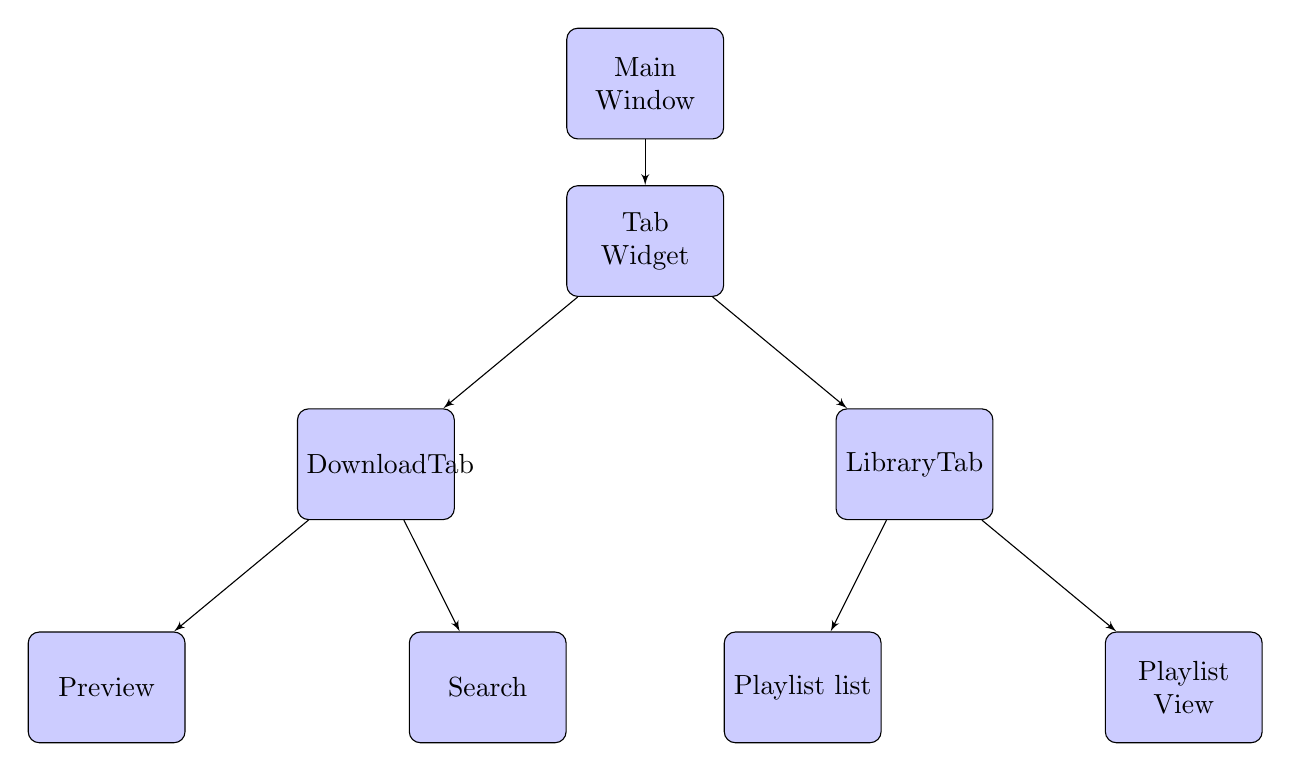
\begin{tikzpicture}[node distance = 2cm, auto]
        % Place nodes
        \node [block] (init) {Main Window};
        \node [block, below of=init] (TabWidget) {Tab Widget};
        \node [block, below left=of TabWidget] (DownloadTab) {DownloadTab};
        \node [block, below right=of TabWidget] (LibraryTab) {LibraryTab};
        \node [block, below left=of DownloadTab] (Preview) {Preview};
        \node [block, fill=none, draw=none, below right=of DownloadTab] (PlaceHolder) {};
        \node [block, left of=PlaceHolder] (Search) {Search};
        \node [block, right of=PlaceHolder] (PlaylistList) {Playlist list};
        \node [block, below right=of LibraryTab] (PlaylistView) {Playlist View};
        % Draw edges \path [line] (init) -- (identify);
        \path [line] (init) -- (TabWidget);
        \path [line] (TabWidget) -- (DownloadTab);
        \path [line] (TabWidget) -- (LibraryTab);
        \path [line] (DownloadTab) -- (Preview);
        \path [line] (DownloadTab) -- (Search);
        \path [line] (LibraryTab) -- (PlaylistList);
        \path [line] (LibraryTab) -- (PlaylistView);
    \end{tikzpicture}
    \caption{Layer Model} \label{fig:Layer Model}
\end{figure}
The two item on the graph above which has the most visual significance would be
DownloadTab and LibraryTab as they are the direct descendants of the Tab Widget.
Due to this fact I think that it is important to layout how I intend this two item to
look. The first that we will look at will be the Download Tab which is shown as Figure
~\ref{fig:DownloadTab Diagram}. There are quite a few objects on this diagram which are
not in the layer model (Fig ~\ref{fig:Layer Model}) these objects are to interact with
the two main widgets on the DownloadTab which are preview and searchlist. As the name
suggests the preview is to allow the user to view the video before downloading while.
Within GUI and network programming you often want one object to be notified when an event
happens to another. Fortunately Qt recognises this problem and has signals and slots to
solve it. To use these you need to use the emit to create a signal and the you can use
a slot to listen out for that signal and run a procedure when that signal is received.
This is vital when interacting with the user as when the user clicks a button or interacts
with the interface a signal is emitted and I need to connect a slot up to these signals
to make the application work.
With this knowledge I can start to explain how all of the classes come together and
function with the figures shown below. All of these figures are annotated and should
explain them in detail. It is important to know that the diagrams only show the
public procedures and functions currently. This is because I want to clearly line
out how they interact with one another. The only figure without this annotation is
figure ~\ref{fig:Struct layout} so I will explain it here. All of the structs that I
am describing occur in the classes VideoYoutube (Fig ~\ref{fig:VideoYoutube class layout})
and HttpHandler (Fig ~\ref{fig:HttpHandler class layout}) and the first to dive into is
download. This struct is to store information about the current downloaded video. The
first property "reply" is to store the response from the http request which will
especially important for checking for errors and making sure it has the right thing. The
next property "tempfile" is important for insurance reasons as the download may be
interrupted causing the file to be corrupt. In order to prevent this I thought it would
be best to create a temporary file that will be automatically deleted by the operating
system after a period of time. This means I can continually put data into this temporary
file and when the download file is finished save it into a permanent file. To have the
correct name to save the file to I have the title property. The "progress",
"currentProgress" and "getProgress" are used to keep track of progress for the download
progress bar. The "segments" and "segmentPosition" is to allow the functionality to
download the video if it is cut into segments. "CurrentStatus" is to get the http status
code. Finally the "download()" procedure is to initiate the download process.
The "fmtQuality" and "videoQuality" structs store the qualities and there relevant
urls. The first property of the "fmtQuality" struct is "quality" which stores the quality
that is listed by youtube. The "resolution", "video" and "audio" properties are to store
their qualities respectively. The procedure "fmtQuality" is the constructor to initialise
all of these properties. The "videoQuality" has the same "quailty" property but also has
"audioUrl" and "videoUrl". These actually store the url to download the video. It should be
noted that I put this property in "videoQuality" instead of "download" because there
multiple urls for a video each different due to the quality. The "videoQuality" procedure
is different ways of initializing the properties and the operator is to compare the
different qualities.
Finally the "jsMethod" struct is to store the the JavaScript code from youtubes code in
order to parse signatures to make the urls valid.
I need to also consider the data structure I am going to use for controlling the order of
the songs that will be played through LibraryTab. There are two data structures which
I am currently considering: Linkedlist and an array.% A comparison table is shown in Fig \ref{fig:Data structure table}.
Based on the the ease of use I
belive that the easier and more efficient option would be to use an array.
%\break
Another key design feature I need to implement is making the use of the program as
intuitive as possible. Because of this I think the best way for the user to insert
songs and reorder them would be through a drag and drop system. This would require
me to set up various variables and features embedded in qt which is described
\href{http://doc.qt.io/qt-5/model-view-programming.html#using-drag-and-drop-with-item-views}
{here}.
\begin{figure}[H]
    \centering
    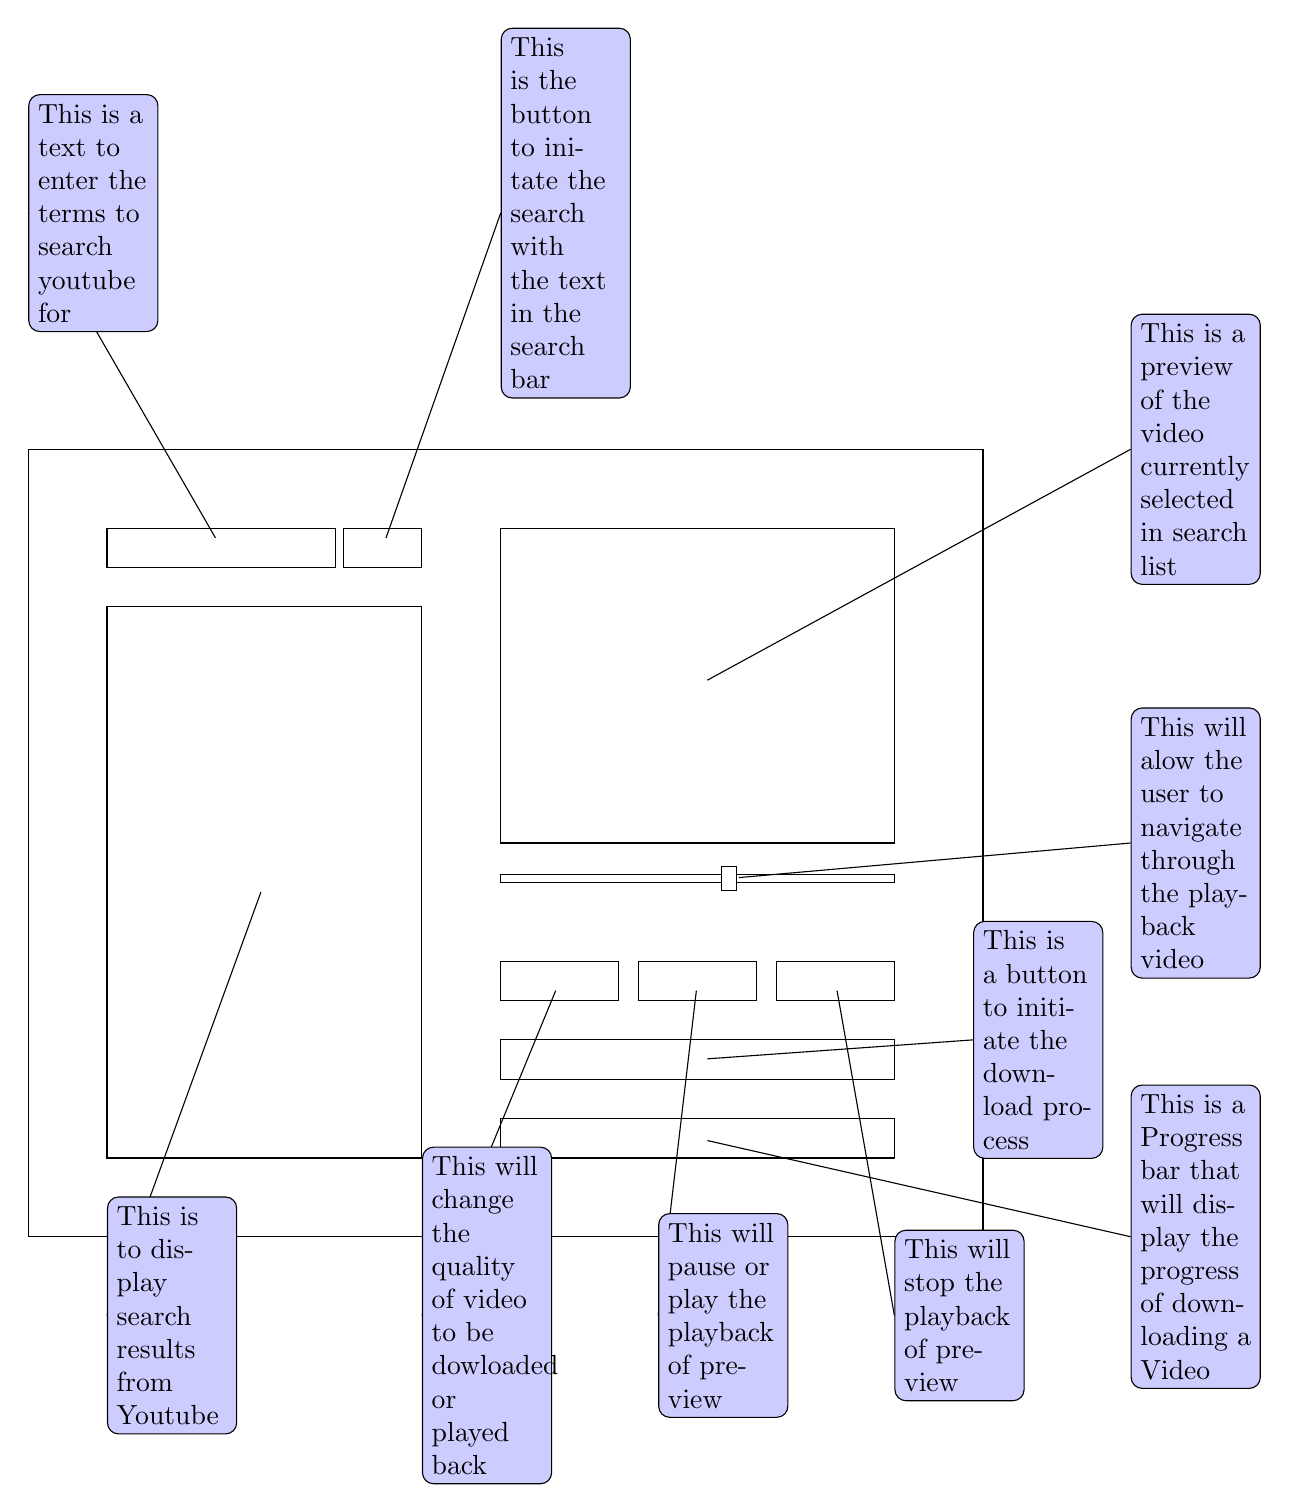
\begin{tikzpicture}[]
        \draw [fill=white] (0,0) rectangle (\textwidth,10) node[pos=0.5] (DownloadTab) {};
        \draw [] (3.9, 8.5) rectangle (1, 9) node[pos=0.5] (SearchBar) {}; %serch bar
        \draw [] (4, 8.5) rectangle (5, 9) node[pos=0.5] (SearchBtn) {}; %search btn
        \draw [] (1, 1) rectangle (5, 8) node[pos=0.5] (SearchList) {}; %search list
        \draw [] (11, 5) rectangle (6, 9) node[pos=0.5] (Preview) {}; %preview
        \draw [] (11, 4.5) rectangle (6, 4.6); %slider body
        \draw [fill=white] (9, 4.4) rectangle (8.8, 4.7) node[pos=0.5] (Slider) {}; %slider handle
        \draw [] (7.5, 3) rectangle (6, 3.5) node[pos=0.5] (QualitySelector) {}; %qualitySelector
        \draw [] (9.25, 3) rectangle (7.75, 3.5) node[pos=0.5] (PlayPauseBtn) {}; %play/pause
        \draw [] (11, 3) rectangle (9.5, 3.5) node[pos=0.5] (StopBtn) {}; %StopBtn
        \draw [] (11, 2) rectangle (6, 2.5) node[pos=0.5] (DownloadBtn) {}; %download btn
        \draw [] (11, 1.5) rectangle (6, 1) node[pos=.5] (ProgressBar) {}; %Progress Bar
        \draw (ProgressBar) -- (14, 0) node[TextBox, pos=1] {
            This is a Progress bar that will display the progress of downloading a Video
        };
        \draw (DownloadBtn) -- (12, 2.5) node[TextBox, pos=1] {
            This is a button to initiate the download process
        };
        \draw (StopBtn) -- (11, -1) node[TextBox, pos=1] {
            This will stop the playback of preview
        };
        \draw (PlayPauseBtn) -- (8, -1) node[TextBox, pos=1] {
            This will pause or play the playback of preview
        };
        \draw (QualitySelector) -- (5, -1) node[TextBox, pos=1] {
            This will change the quality of video to be dowloaded or played back
        };
        \draw (SearchList) -- (1, -1) node[TextBox, pos=1] {
            This is to display search results from Youtube
        };
        \draw (Slider) -- (14, 5) node[TextBox, pos=1] {
            This will alow the user to navigate through the playback video
        };
        \draw (Preview) -- (14, 10) node[TextBox, pos=1] {
            This is a preview of the video currently selected in search list
        };
        \draw (SearchBtn) -- (6, 13) node[TextBox, pos=1] {
            This is the button to initate the search with the text in the search bar
        };
        \draw (SearchBar) -- (0, 13) node[TextBox, pos=1] {
            This is a text to enter the terms to search youtube for
        };
    \end{tikzpicture}
    \caption{DownloadTab Diagram} \label{fig:DownloadTab Diagram}
\end{figure}
\begin{figure}[H]
    \centering
    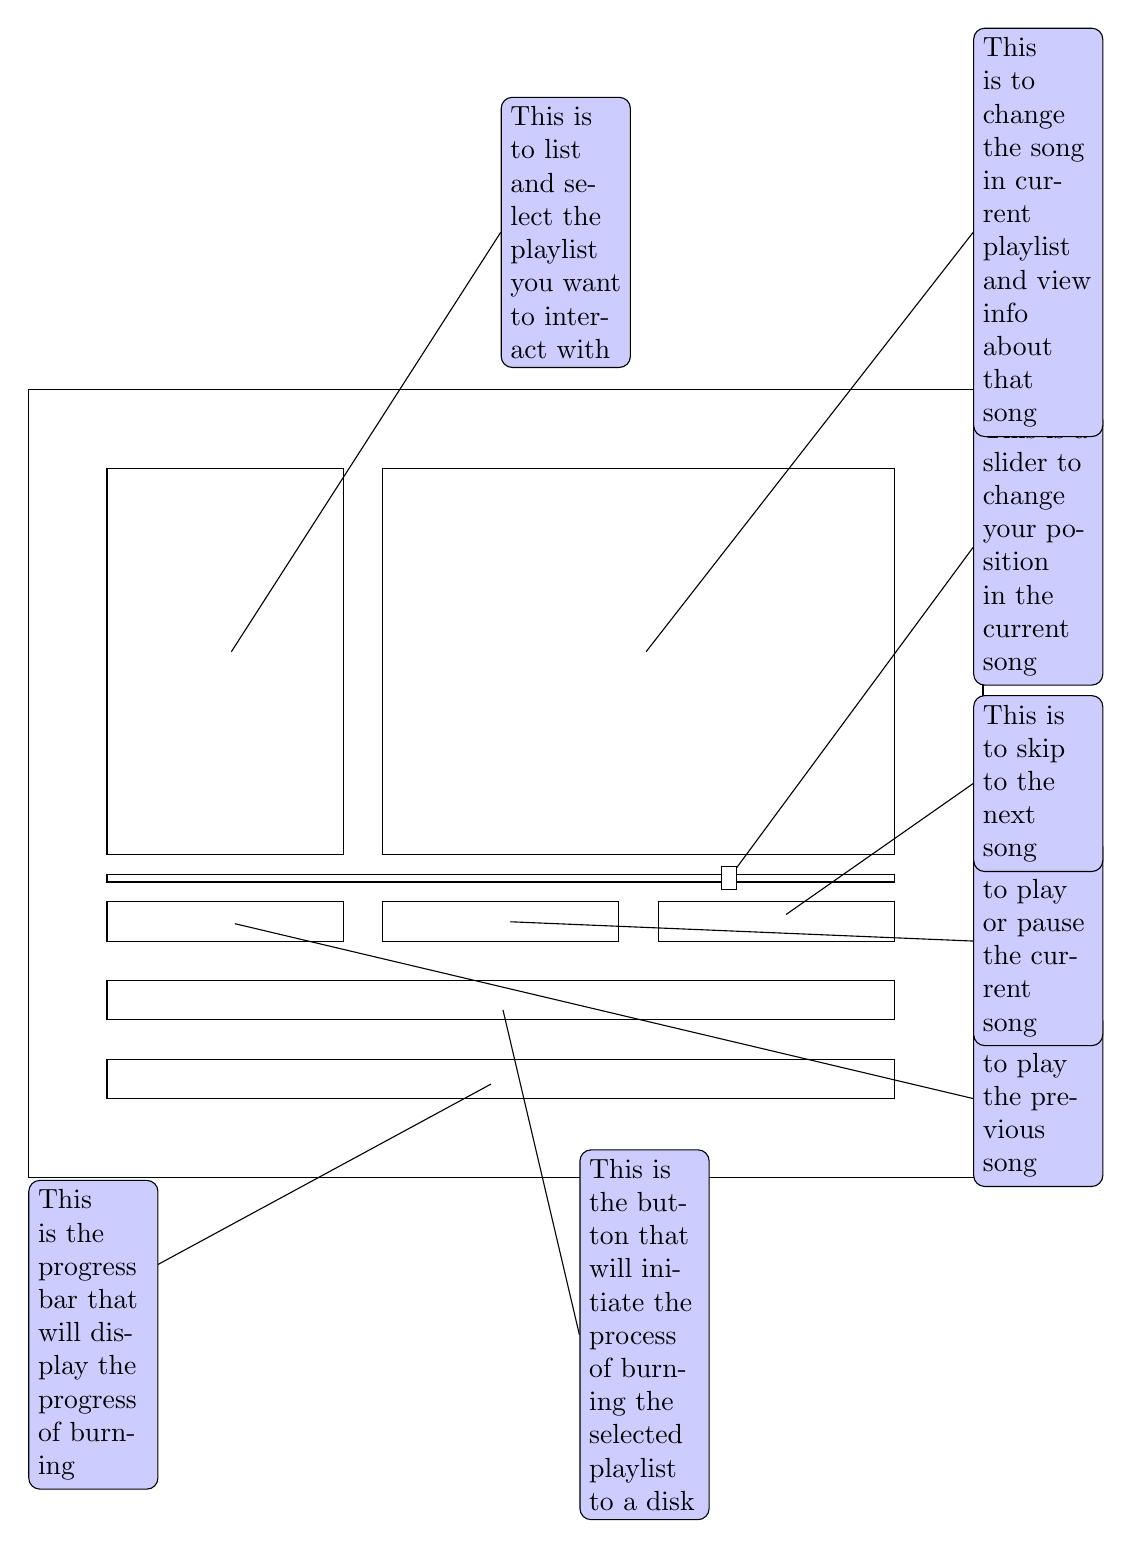
\begin{tikzpicture}[]
        \draw [] (0,0) rectangle (\textwidth, 10);
        \draw [] (1, 9) rectangle (4, 4.1) node[pos=0.5] (PlaylistListing) {}; %Playlist listing
        \draw [] (4.5, 9) rectangle (11, 4.1) node[pos=0.5] (SongSelector) {}; %Song selector
        \draw [] (11, 3.75) rectangle (1, 3.85); %slider body
        \draw [fill=white] (9, 3.65) rectangle (8.8, 3.95) node[pos=0.5] (Slider) {}; %slider handle
        \draw [] (4, 3) rectangle (1, 3.5) node[pos=0.5] (Prev) {}; %prev Btn
        \draw [] (4.5, 3) rectangle (7.5, 3.5) node[pos=0.5] (PlayPause) {}; %play/pause
        \draw [] (11, 3) rectangle (8, 3.5) node[pos=0.5] (Next) {}; %next btn
        \draw [] (11, 2) rectangle (1, 2.5) node[pos=0.5] (BurnBtn) {}; %Burn btn
        \draw [] (11, 1.5) rectangle (1, 1) node[pos=.5] (ProgressBar) {}; %Progress
        \draw (ProgressBar) -- (0, -2) node[TextBox, pos=1] {
            This is the progress bar that will display the progress of burning
        };
        \draw (BurnBtn) -- (7, -2) node[TextBox, pos=1] {
            This is the button that will initiate the process of burning the selected playlist to a disk
        };
        \draw (Prev) -- (12, 1) node[TextBox, pos=1] {
            This is to play the previous song
        };
        \draw (PlayPause) -- (12, 3) node[TextBox, pos=1] {
            This is to play or pause the current song
        };
        \draw (Next) -- (12, 5) node[TextBox, pos=1] {
            This is to skip to the next song
        };
        \draw (Slider) -- (12, 8) node[TextBox, pos=1] {
            This is a slider to change your position in the current song
        };
        \draw (SongSelector) -- (12, 12) node[TextBox, pos=1] {
            This is to change the song in current playlist and view info about that song
        };
        \draw (PlaylistListing) -- (6, 12) node[TextBox, pos=1] {
            This is to list and select the playlist you want to interact with
        };
    \end{tikzpicture}
    \caption{LibraryTab Diagram} \label{fig:LibraryTab Diagram}
\end{figure}
\begin{figure}[H]
    \centering
    \begin{tikzpicture}
        \begin{sideways}
            \node [] (tree) at (4, 4) {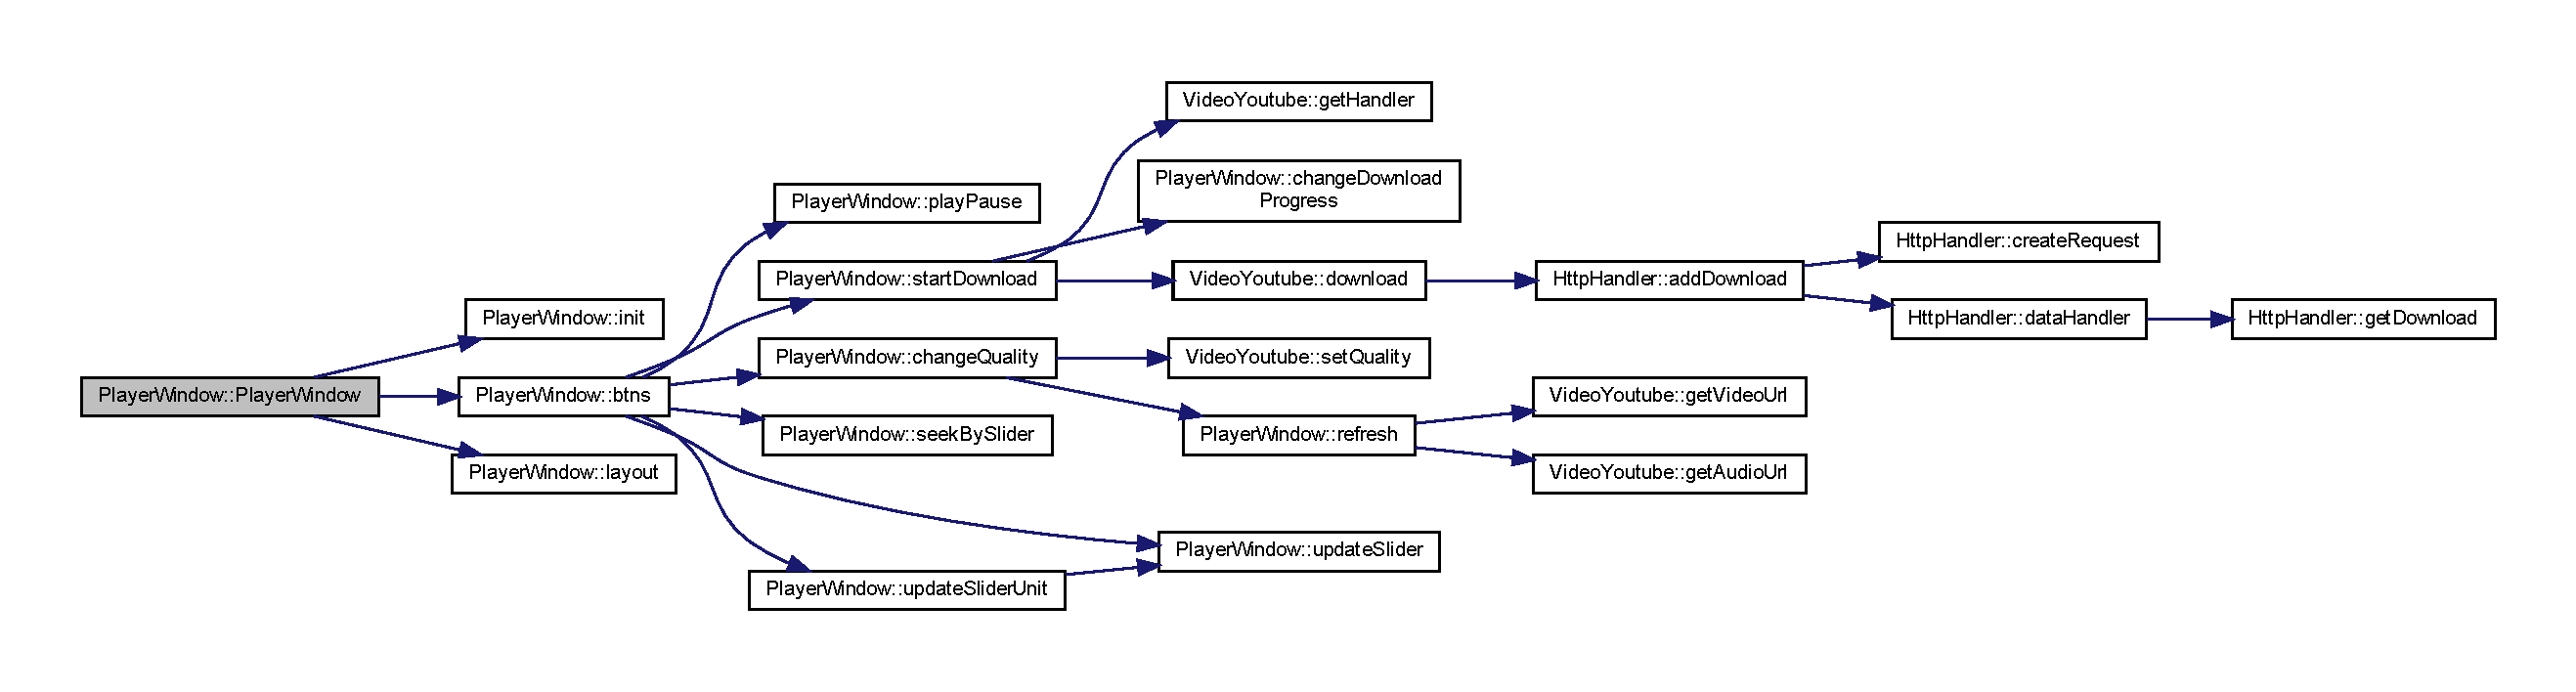
\includegraphics[width=\textheight]{classPdfs/classPlayerWindow_a88bd0544109c4b49dbba0adc29c16943_cgraph.pdf}};
        \end{sideways}
        \node [right of = tree] (inherit) {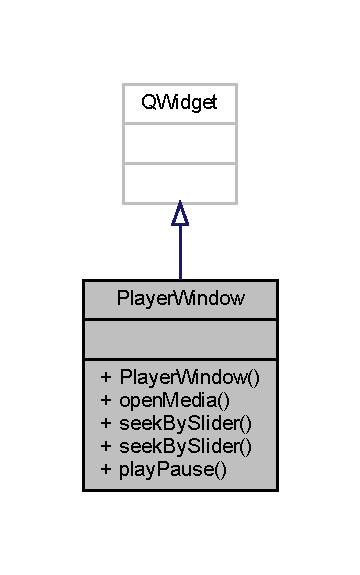
\includegraphics[]{classPdfs/classPlayerWindow.pdf}};
        \node [TextBox, above=0cm of inherit, text width = 30em] (textbox) {
            The class will be used to play media selected by the user and provide
            controls. This will be on both DownloadTab and LibraryTab meaning that
            the constructor will be called in both of these classes. The tree on the
            left describes what happens when you call the constructor. Since this is a
            class that will be visually displayed to the user this class inherits the
            QWidget. It also has the openMedia() procedure which is call by downloadtab
            to set the media after extracting the URL. Finally the seekBySlider and
            playPause are for the user to control the media.
        };
    \end{tikzpicture}
    \caption{PlayWindow class layout} \label{fig:PlayWindow class layout}
\end{figure}
\begin{figure}[H]
    \centering
    \begin{tikzpicture}
        \begin{sideways}
            \node [] (tree) at (4, 4) {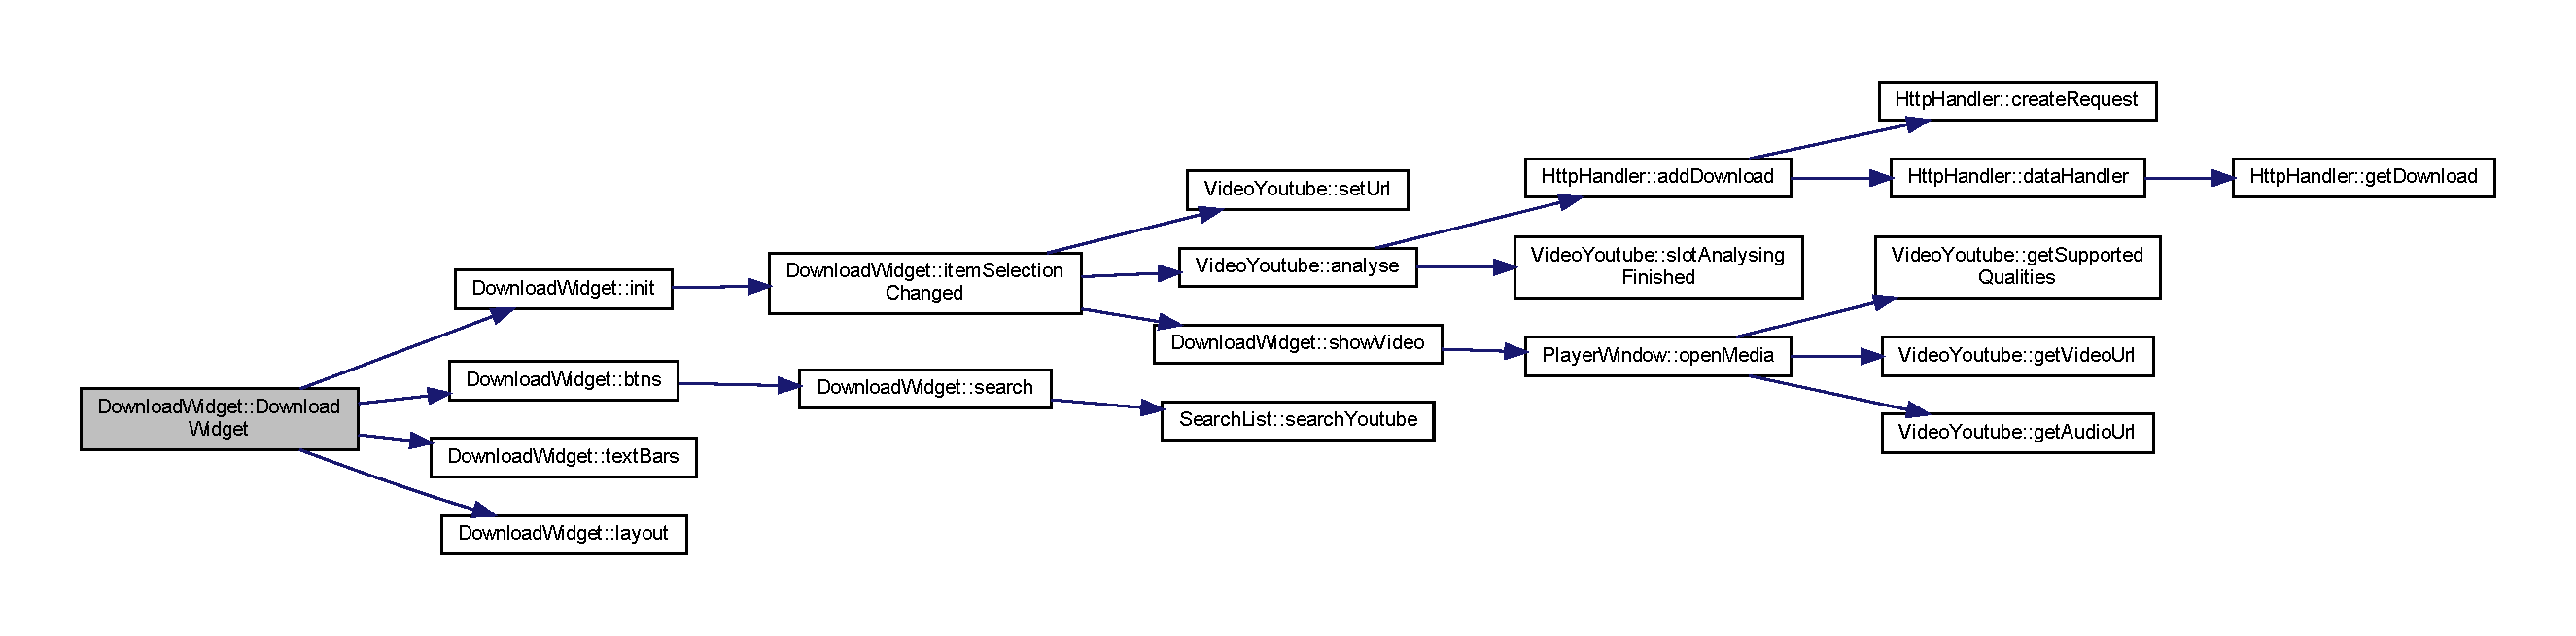
\includegraphics[width=\textheight]{classPdfs/classDownloadWidget_a623f84423fc0163ff5cd6b75000fffd5_cgraph.pdf}};
        \end{sideways}
        \node [right of = tree] (inherit) {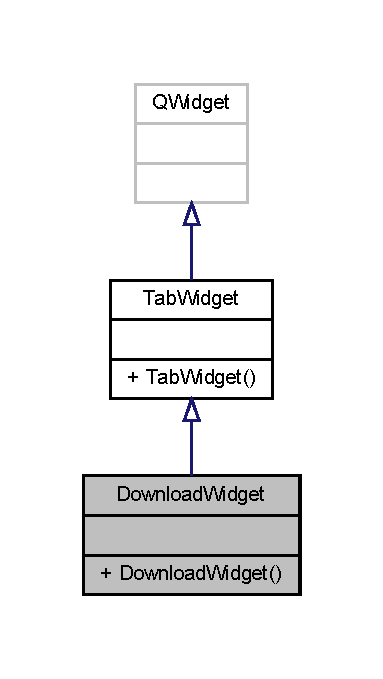
\includegraphics[]{classPdfs/classDownloadWidget.pdf}};
        \node [TextBox, above=0cm of inherit, text width = 30em] (textbox) {
        	The DownloadWidget class will be used to create the DownloadTab object. This
        	object will provide a canvas to put all of the features described in the
        	downloadTab diagram (Fig ~\ref{fig:DownloadTab Diagram}). It should be noted
        	this inherits from the TabWidget meaning it will be added as a tab
        	automatically. The constructor will be called from the MainWindow. Finally
        	this class will act as a middle man for other classes like PlayerWindow
        	(Fig ~\ref{fig:PlayWindow class layout}).
        };
    \end{tikzpicture}
    \caption{DownloadWidget class layout} \label{fig:DownloadWidget class layout}
\end{figure}
\begin{figure}[H]
    \centering
    \begin{tikzpicture}
        \begin{sideways}
            \node [] (tree) at (4, 4) {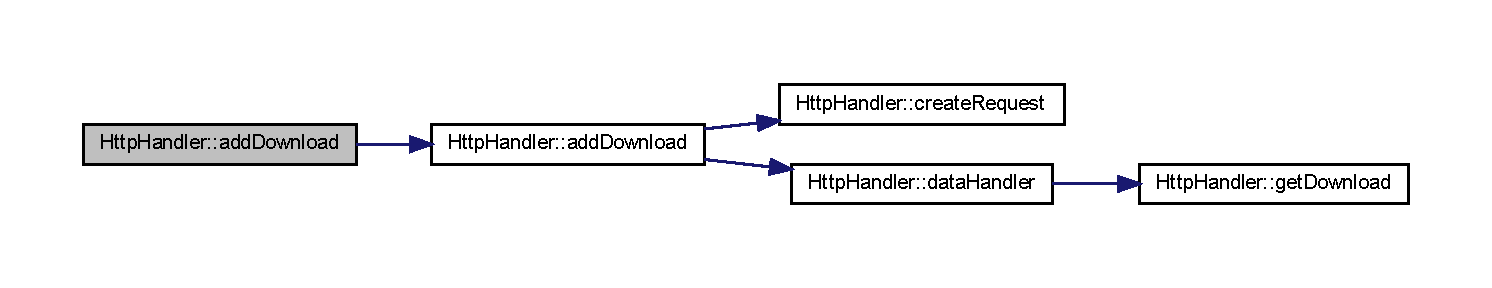
\includegraphics[width=\textheight]{classPdfs/classHttpHandler_ade64572cb953620fd483bc669c1e9178_cgraph.pdf}};
        \end{sideways}
        \node [right of = tree] (inherit) {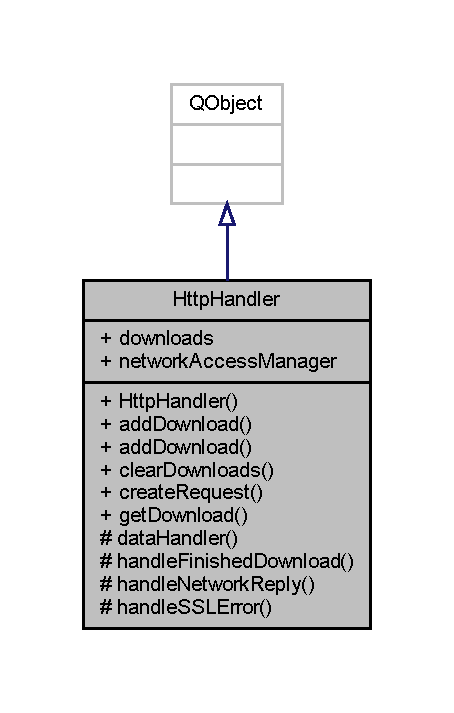
\includegraphics[]{classPdfs/classHttpHandler.pdf}};
        \node [TextBox, above=0cm of inherit, text width = 30em] (textbox) {
        	For this class the first thing that you know is that it inherits from QObject
        	instead of QWidget or a derivative of QWidget. This means that this class
        	has no visual representation but completely backend. The point of this class
        	is to perform all of the networking required. I decided to put all of it
        	into a separate class because many errors can occur with network requests
        	so proper error handling is a must. Due to the fact that you often have to
        	wait for network requests to finished this class has numerous slots like
        	dataHandler to process the the finished download. The final two things that
        	should be noted is the data members downloads and networkAcessManager.
        	The member downloads is a QList of the download struct, see (Fig ). The
        	networkAcessManager is a QNetworkManager which is Qt class that allows
        	you to make network requests.
        };
    \end{tikzpicture}
    \caption{HttpHandler class layout} \label{fig:HttpHandler class layout}
\end{figure}
\begin{figure}[H]
    \centering
    \begin{tikzpicture}
        \begin{sideways}
            \node [] (tree) at (4, 4) {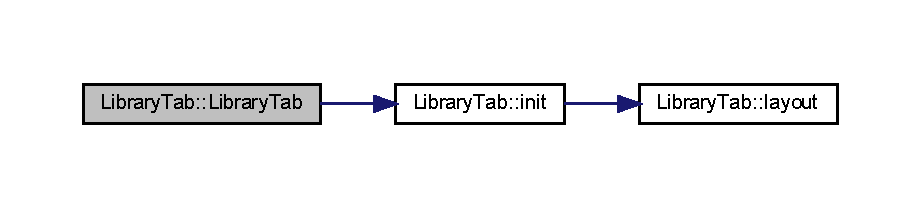
\includegraphics[width=\textheight]{classPdfs/classLibraryTab_a928c981ca174c41d75e5296d4623d5a2_cgraph.pdf}};
        \end{sideways}
        \node [right of = tree] (inherit) {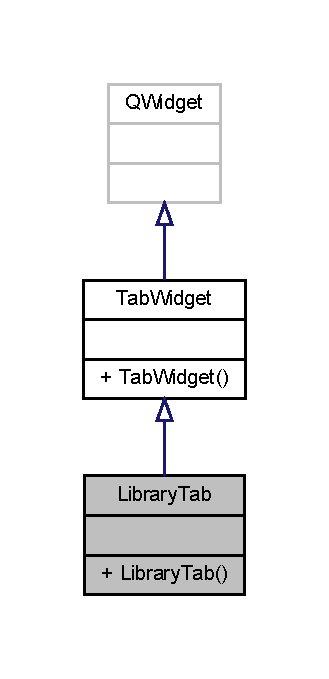
\includegraphics[]{classPdfs/classLibraryTab.pdf}};
        \node [TextBox, above=0cm of inherit, text width = 30em] (textbox) {
        	Similarly to DownloadWidget this is a child of TabWidget meaning it is one
        	of the two tabs and provides a canvas to put widgets on. Fig
        	\ref{fig:LibraryTab Diagram} shows how intend it to look. This class
        	will be the middle man for all of the data handling. Within the
        	constructor all of the objects shown in Fig \ref{fig:LibraryTab Diagram}
        	will be initialized and then layerd out in the layout procedure.
        };
    \end{tikzpicture}
    \caption{LibraryTab class layout} \label{fig:LibraryTab class layout}
\end{figure}
\begin{figure}[H]
    \centering
    \begin{tikzpicture}
        \begin{sideways}
            \node [] (tree) at (4, 4) {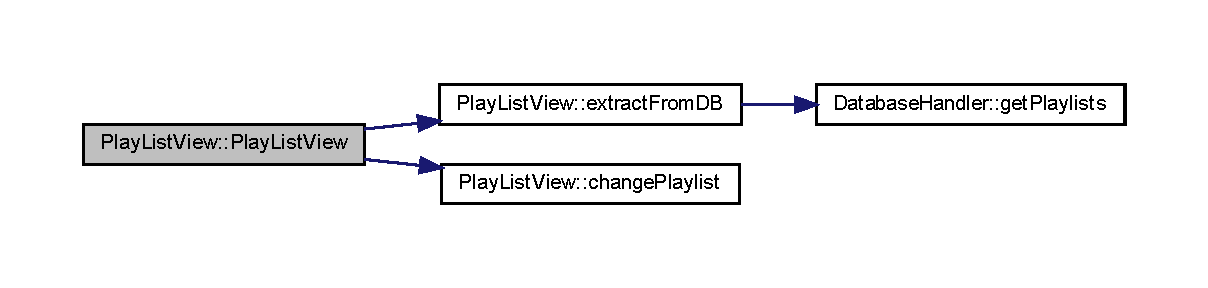
\includegraphics[width=\textheight]{classPdfs/classPlayListView_ac84c4c57fc29e6b775c2bc8bc5fed55e_cgraph.pdf}};
        \end{sideways}
        \node [right of = tree] (inherit) {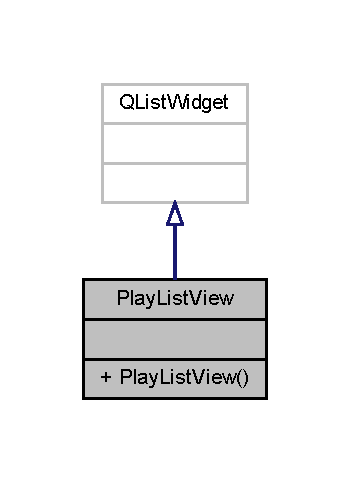
\includegraphics[]{classPdfs/classPlayListView.pdf}};
        \node [TextBox, above=0cm of inherit, text width = 30em] (textbox) {
			This class is called by LibraryWidget and is used to list the playlists
			that the user has and allow the user to place songs and edit the playlists.
			It should be noted that instead of a standard QWidget being used a QListWidget
			is used. This still has a visual representation but instead of being a blank
			canvas it lists items that you can add with the addItem procedure.
        };
    \end{tikzpicture}
    \caption{PlaylistView class layout} \label{fig:PlaylistView class layout}
\end{figure}
\begin{figure}[H]
    \centering
    \begin{tikzpicture}
        \node [right of = tree] (inherit) {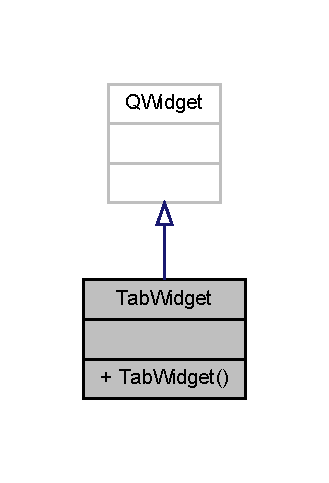
\includegraphics[]{classPdfs/classTabWidget.pdf}};
        \node [TextBox, above=0cm of inherit, text width = 30em] (textbox) {
			Unlike the other class this class is abstract. This means that it should
			always be a parent class in use and never called directly. The reasoning
			behind this is that I want a way that I could add classes automatically.
			This would also mean that if in the future I want to style my tabs I can
			easily do so by applying styles to this which would apply to the children.
        };
    \end{tikzpicture}
    \caption{TabWidget class layout} \label{fig:TabWidget class layout}
\end{figure}
\begin{figure}[H]
    \centering
    \begin{tikzpicture}
        \begin{sideways}
            \node [] (tree) at (4, 4) {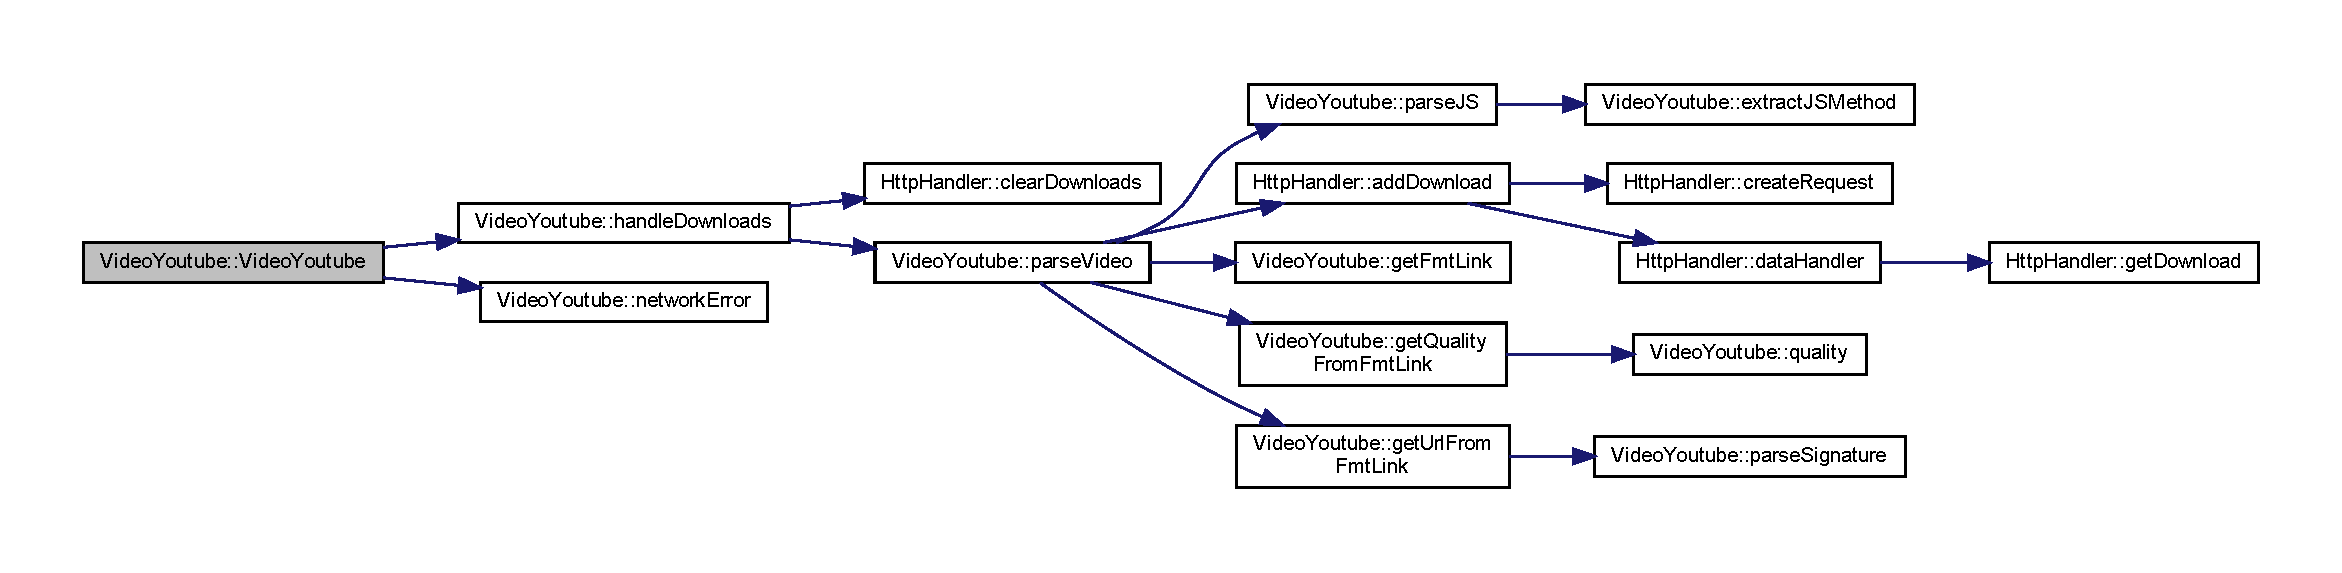
\includegraphics[width=\textheight]{classPdfs/classVideoYoutube_a80afcc31ca007b32108976d2158be9ce_cgraph.pdf}};
        \end{sideways}
        \node [right of = tree] (inherit) {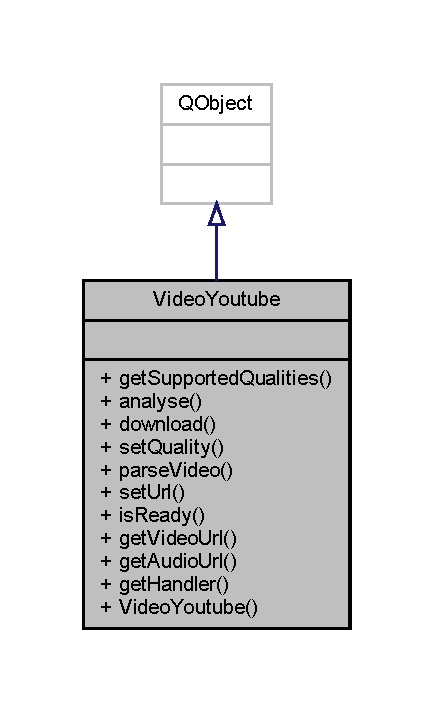
\includegraphics[]{classPdfs/classVideoYoutube.pdf}};
        \node [TextBox, above=0cm of inherit, text width = 30em] (textbox) {
			This class is used to represent the currently selected video from the
			search on the download tab. The main objective of this class is with the
			use of HttpHandler (Fig \ref{fig:HttpHandler class layout}) to extract the
			url of the actual youtube video which is done in the parseVideo procedure.
			Once the url has been retrieved the getVideoUrl and the getAudioUrl functions
			provide objects like preview the url to play the video. The download procedure
			will pass the audio url onto the HttpHandler so that it can be downloaded
			and added to the database. Finally to repeat the process you need to set
			a new webpage url with setUrl and call the analyse procedure.
        };
    \end{tikzpicture}
    \caption{VideoYoutube class layout} \label{fig:VideoYoutube class layout}
\end{figure}
\begin{figure}[H]
    \centering
    \begin{tikzpicture}
        \begin{sideways}
            \node [] (tree) at (4, 4) {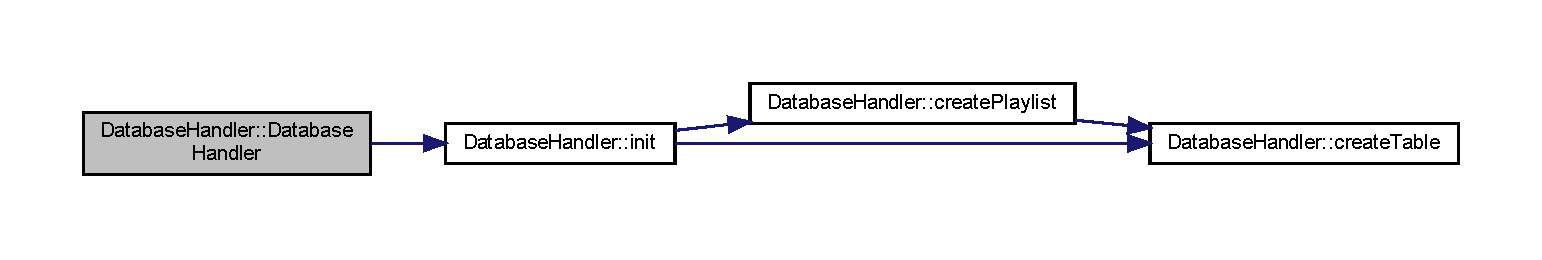
\includegraphics[width=\textheight]{classPdfs/classDatabaseHandler_a6f3d7ae8a73f534059dc5667b29eb0d2_cgraph.pdf}};
        \end{sideways}
        \node [right of = tree] (inherit) {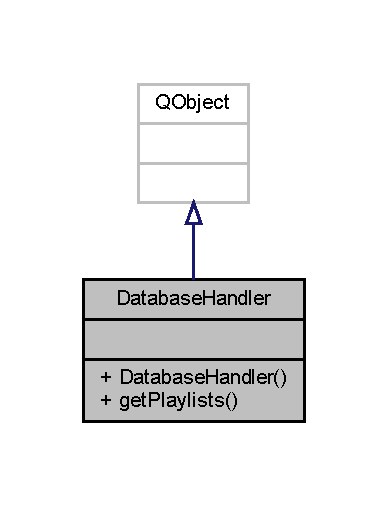
\includegraphics[]{classPdfs/classDatabaseHandler.pdf}};
        \node [TextBox, above=0cm of inherit, text width = 30em] (textbox) {
			This class is meant to handle all of the database function and is called
			by the LibraryWidget class. The should create all of the tables needed to
			represent the tables and organise everything. Like the HttpHandler class
			this class is a child of QObject showing that it is completely backend
			and has no visual representation.
        };
    \end{tikzpicture}
    \caption{DatabaseHandler class layout} \label{fig:DatabaseHandler class layout}
\end{figure}
\begin{figure}[H]
    \begin{tikzpicture}[node distance=\textwidth /3]
        \node [] (download) {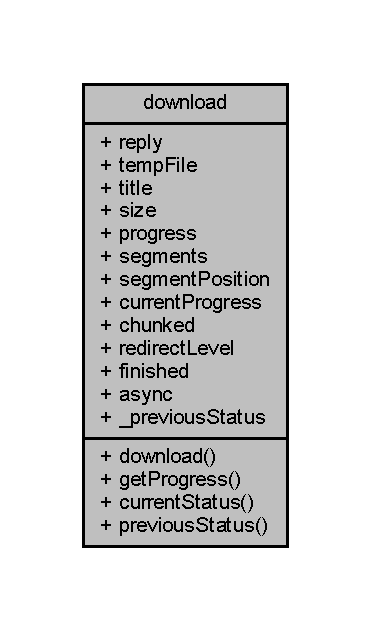
\includegraphics{classPdfs/structdownload}};
        \node [right of=download] (fmtQuality) {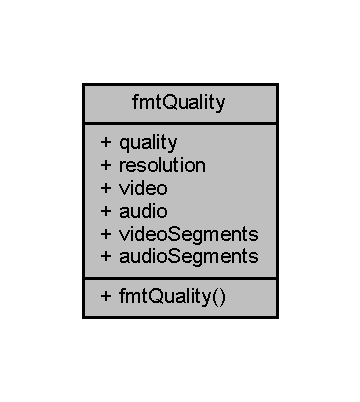
\includegraphics{classPdfs/structfmtQuality}};
        \node [below=0.0mm of  download.south] (videoQuality) {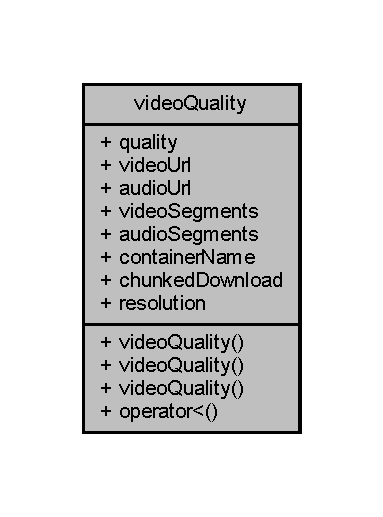
\includegraphics{classPdfs/structvideoQuality}};
        \node [right of=videoQuality] (jsMethod) {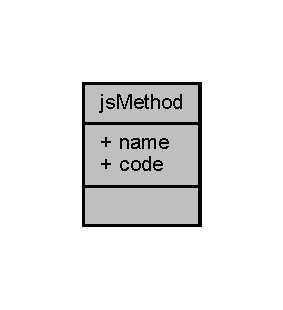
\includegraphics{classPdfs/structjsMethod}};
    \end{tikzpicture}
    \caption{Struct layout} \label{fig:Struct layout}
\end{figure}
\break
\subsection{DatabaseHandling}\label{DatabaseHandling}
As mention previously I decided that I would use a database to keep track of the
downloaded music. To do this I will have one main table that will have any
downloaded song automatically inserted into it. This table will be called "AllSongs"
. This "AllSongs" table with contain 5 columns which I will describe here.
The first column is the "id" columns which will be use to order the data
and to refrence the data inside "AllSongs". Because of this id will be an
integear with each one being unique and auto increment. The second column
is "TrackName" which as the title suggest will be a text field containing
the name of the download song. The next two columns will be "artists" and
"genre" which will both be integers to reference values in the artist and
genre tables. This will avoid duplicates. These tables will have an id field
identical to the AllSongs table and the artist and genre columns will
reference values using this field. Finally there will be the duration
file which is a double that will hold the length of the song in minuets.
To further avoid duplications any playlist created by the user will reference
the songs in "AllSongs".In order to allow these references I will need to use join
statements in sql. I need to use this statement as I still want the artist and
genre columns in the users playlist without having to create this additional columns.
By using select with these join statement along with the where clause I should
be able to grab all data that has the same id.
A requirement by my client is the ability to reorder the songs. My approach
to this is to switch the id of the two songs to switch them in the view.
Due to both id's having the unique property I will need to use the id as
0 for a temp value. This should be relatively simple with sql update statements
Another database quirk that I need to take into consideration is when the user
deletes a song in the playlist as this will cause there to be gaps in the
ids of tables. This is problematic as I cannot get the right id by getting
the rowid. There are two ways I could solve this: I update all of the ids
greater that the deleted item so there are no gaps or allow gaps and find
a way of selecting a row of data in the database by how far down it is.
The first option is a bad idea as this means changing id which are going
to be used as relations and it may become time consuming for large
amount of rows. The second option is much better but I was original unsure
of how to achieve it untill I discovered the "OFFSET" clause. With this
I can offset a select statement n rows down the table making this task
trivial.
With this knowledge I have created a table below in figure ~\ref{fig:SQLTable}
that I belive I will need for the database.
\begin{figure}[H]
    \begin{center}
        \begin{tabular} { | c | c | }
            \hline
            \textbf{Query}                   &                 \textbf{Summerary}             \\ \hline
            CREATE TABLE IF NOT EXISTS       &This should create the artists table. This      \\
            artists(id INTEGEAR NOT NULL     &will store the artists name and an id to        \\
            PRIMARY KEY AUTOINCREMENT UNIQUE,&reference the name                              \\
            artist TEXT)                     &                                                \\ \hline
            CREATE TABLE IF NOT EXISTS       &This should create the albums table which will  \\
            albums (id INTEGEAR NOT NULL     &store the album name and an id to reference the \\
            PRIMARY KEY AUTOINCREMENT UNIQUE,&name.                                           \\
            albums TEXT)                     &                                                \\ \hline
            CREATE TABLE IF NOT EXISTS       &                                                \\
            AllSongs ( id INTEGEAR NOT NULL  &This should create the AllSongs table which will\\
            PRIMARY KEY AUTOINCREMENT UNIQUE,&be used to store any downloaded song and        \\
            trackName TEXT, artist INTEGEAR, &will be referenced by other playlists.          \\
            Genere INTEGEAR, Duration DOUBLE)&                                                \\ \hline
            DELETE FROM tableName WHERE id   &This statement will be used to allow the user   \\
            IN (SELECT id FROM tableName     &to delete a row from tableName using the number \\
            ORDER BY id LIMIT 1 OFFSET rowId &of rows down in the tableView. It should be     \\
                                             ¬ed that tableName and rowId will be          \\
                                             &substituted at runtime with the appropiate      \\
                                             &values.                                         \\ \hline
            SELECT AllSongs.id, trackName,   &This query will be used to get the appropiate   \\
            artist, Genere, Duration FROM    &data from AllSongs by using the ids in tableName\\
            AllSongs tableName ON AllSongs.id&to reference the values. It should be noted that\\
             = tableName.id                  &tableName is a variable that will be substituted\\
                                             &with the correct value at runtime.              \\ \hline
        \end{tabular}
    \end{center}
    \caption{SQL queries} \label{fig:SQLTable}
\end{figure}
\subsection{NetworkHandling}\label{NetworkHandling}
As remarked previously a key part to this project is the process
of extracting the video url from youtube so it can be previewed
and the sound be downloaded. This section describes this process.
\begin{figure}[H]
    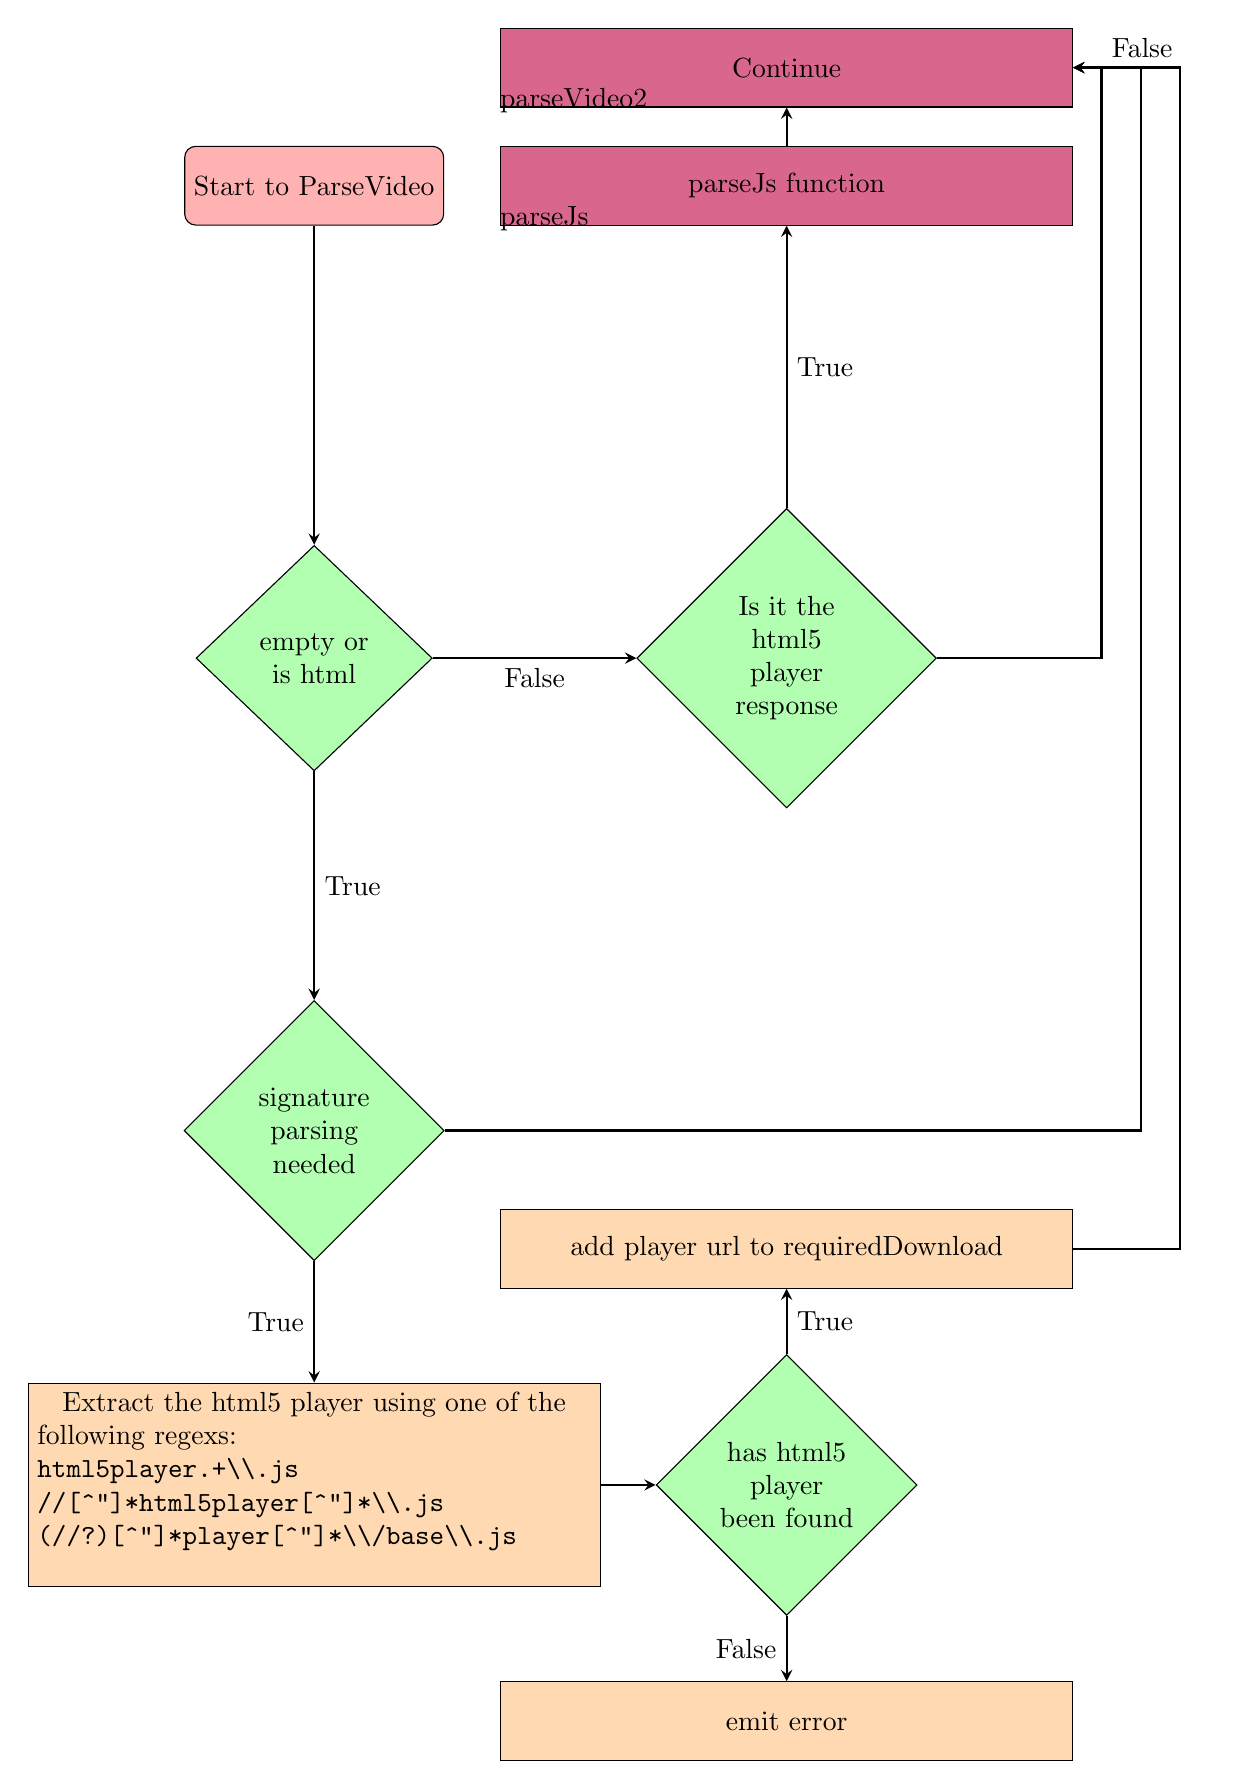
\begin{tikzpicture}[node distance=6cm]
        \node (start) [startstop] {Start to ParseVideo};
        %This is for ifHtml if statement
        \node (ifHtml) [decision, below of=start] {empty or is html};
        \node (ifSigparse) [decision, below of=ifHtml] {signature parsing needed};
        \node (ifJs) [decision, right of=ifHtml] {Is it the html5 player response};
        \draw [arrow] (start) -- node {} (ifHtml);
        \draw [arrow] (ifHtml) -- node[anchor=west] {True} (ifSigparse);
        \draw [arrow] (ifHtml) -- node[anchor=north] {False} (ifJs);
        \node (getHtmlPlayer) [process, yshift=1.5cm, below of=ifSigparse] {
                Extract the html5 player using one of the following regexs:\newline
                \verb!html5player.+\\.js!\newline
                \verb!//[^"]*html5player[^"]*\\.js!\newline
                \verb!(//?)[^"]*player[^"]*\\/base\\.js!\newline
        };
        \draw [arrow] (ifSigparse) -- node[anchor=east] {True} (getHtmlPlayer);
        %This is the ifHtmlPlayer if statement
        \node (ifHtmlPlayer) [decision, right of=getHtmlPlayer] {has html5 player been found};
        \node (html5PlayerFalsetFound) [process, yshift=3cm, below of=ifHtmlPlayer] {emit error};
        \node (html5PlayerFound) [process, yshift=-3cm, above of=ifHtmlPlayer] {add player url to requiredDownload};
        \draw [arrow] (getHtmlPlayer) -- node {} (ifHtmlPlayer);
        \draw [arrow] (ifHtmlPlayer) -- node[anchor=west] {True} (html5PlayerFound);
        \draw [arrow] (ifHtmlPlayer) -- node[anchor=east] {False} (html5PlayerFalsetFound);
        %js player if statement
        \node (parseJs) [process, hyperlink node=parseJs, fill=purple!60, above of=ifJs] {parseJs function};
        \draw [arrow] (ifJs) -- node[anchor=west] {True} (parseJs);
        \node (continue) [process, yshift=-4.5cm, hyperlink node=parseVideo2, fill=purple!60, above of=parseJs] {Continue};
        \draw [arrow] (parseJs) -- node {} (continue);
        \draw [arrow] (html5PlayerFound) -- +(5,0) |- node {} (continue);
        \draw [arrow] (ifJs)  -- +(4,0) |- node[anchor=south west] {False} (continue);
        \draw [arrow] (ifSigparse) -- +(10.5,0) |- node[anchor=east] {} (continue);
    \end{tikzpicture}[node distance=6cm]
    \caption{Start of parse Video} \label{fig:parseVideoStart}
\end{figure}
\begin{figure}[H]
    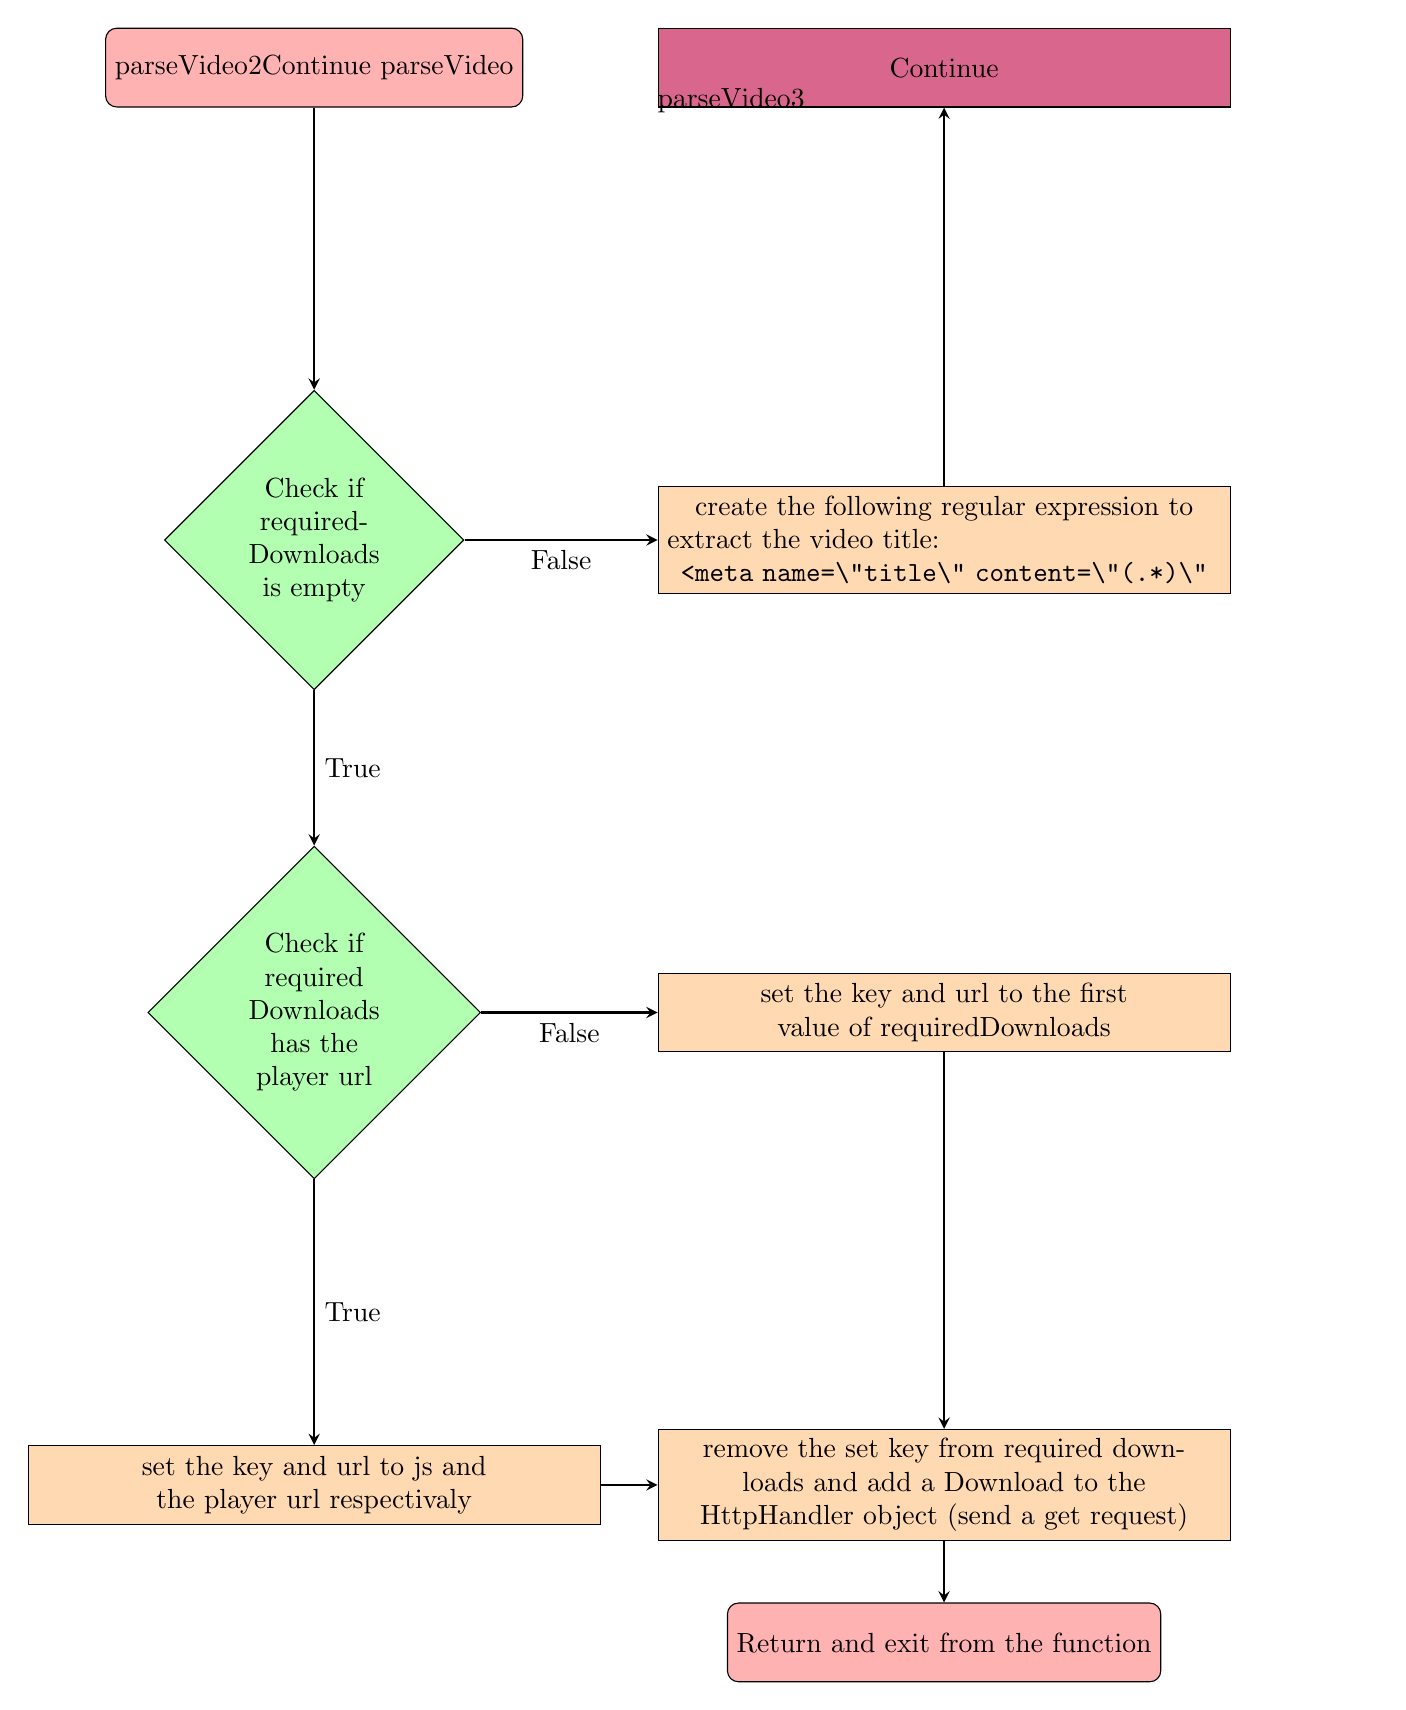
\begin{tikzpicture}[node distance=6cm]
        \node (start) [startstop] {\hypertarget{parseVideo2}{Continue parseVideo}};
        \node (checkForRequiredDownloads) [decision, below of=start] {Check if requiredDownloads is empty};
        \node (checkIfRequiredDownloadsHasJs) [decision, below of=checkForRequiredDownloads] {
            Check if required Downloads has the player url};
        \node (jsIsTrue) [process, below of=checkIfRequiredDownloadsHasJs] {set the key and url
            to js and the player url respectivaly};
        \node (jsIsFalse) [process, xshift=2cm, right of=checkIfRequiredDownloadsHasJs] {set the key and url
            to the first value of requiredDownloads};
        \node (addDownload) [process, below of=jsIsFalse] {remove the set key from
            required downloads and add a Download to the HttpHandler object (send a get request)};
        \node (return) [startstop, yshift=4cm, below of=addDownload] {Return and exit from the
            function};
        \node (titleRegex) [process, above of=jsIsFalse] {create the following regular expression
                to extract the video title:\newline
            \verb!<meta name=\"title\" content=\"(.*)\"!};
        \node (continue) [process, hyperlink node=parseVideo3, fill=purple!60,
            above of=titleRegex] {Continue};
        \draw [arrow] (start) -- node {} (checkForRequiredDownloads);
        \draw [arrow] (checkForRequiredDownloads) -- node[anchor=west] {True}
            (checkIfRequiredDownloadsHasJs);
        \draw [arrow] (checkForRequiredDownloads) -- node[anchor=north] {False} (titleRegex);
        \draw [arrow] (checkIfRequiredDownloadsHasJs) -- node[anchor=west] {True} (jsIsTrue);
        \draw [arrow] (checkIfRequiredDownloadsHasJs) -- node[anchor=north] {False} (jsIsFalse);
        \draw [arrow] (jsIsFalse) -- node {} (addDownload);
        \draw [arrow] (jsIsTrue) -- node {} (addDownload);
        \draw [arrow] (addDownload) -- node {} (return);
        \draw [arrow] (titleRegex) -- node {} (continue);
    \end{tikzpicture}
\end{figure}
\begin{figure}[H]
    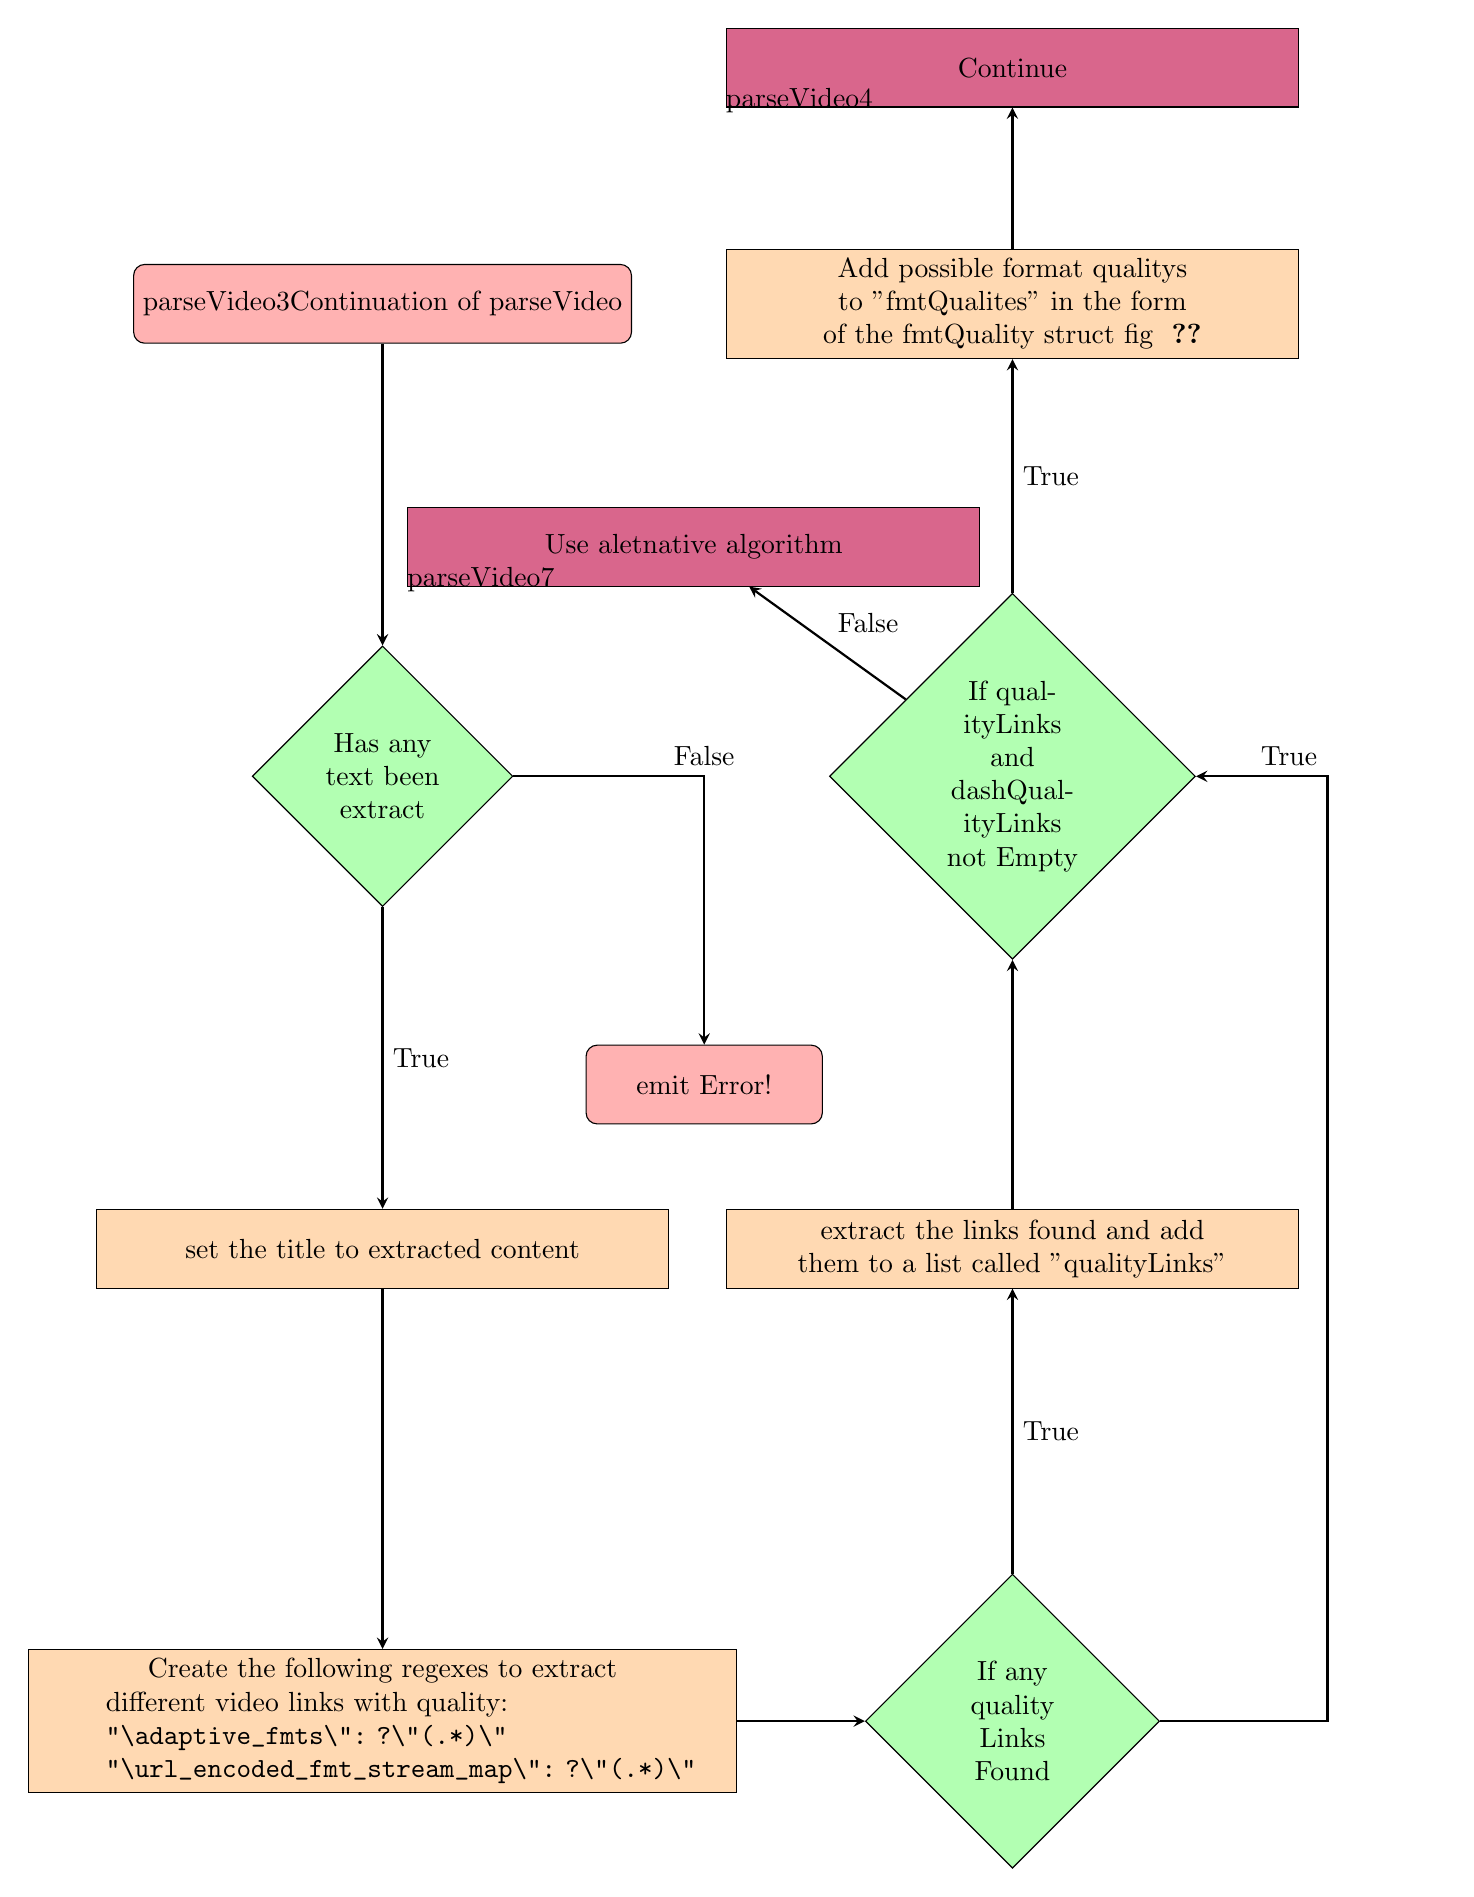
\begin{tikzpicture}[node distance=6cm]
        \node (start) [startstop] {\hypertarget{parseVideo3}{Continuation of parseVideo}};
        \node (ifFoundTitle) [decision, below of=start] {Has any text been extract};
        \node (setTitle) [process, below of=ifFoundTitle] {set the title to extracted content};
        \node (qualityLinkRegex) [process, minimum width=9cm, below of=setTitle] {Create the
            following regexes to extract different video links with quality:\newline
            \verb!"\adaptive_fmts\": ?\"(.*)\"!\newline
            \verb!"\url_encoded_fmt_stream_map\": ?\"(.*)\"!};
        \node (ifQualityLinksFound) [decision, xshift=2cm, right of=qualityLinkRegex] {If any
            quality Links Found};
        \node (QualityLinksFound) [process, above of=ifQualityLinksFound] {extract the links
            found and add them to a list called "qualityLinks"};
        \node (ifQualityLinksIsNotEmpty) [decision, above of=QualityLinksFound] {If
            qualityLinks and dashQualityLinks not Empty};
        \node (alternativeMethod) [process, yshift=-3cm, xshift=5cm, hyperlink node=parseVideo7, fill=purple!60,
            above left =of ifQualityLinksIsNotEmpty] {Use aletnative algorithm};
        \node (qualityHasItems) [process, above of=ifQualityLinksIsNotEmpty] {Add possible
            format qualitys to "fmtQualites" in the form of the fmtQuality struct fig
            ~\ref{fig:Struct layout}};
        \node (error) [startstop, xshift=3cm, yshift=2cm,
            below left =of ifQualityLinksIsNotEmpty] {emit Error!};
        \node (continue) [process, yshift=-3cm, hyperlink node=parseVideo4, fill=purple!60,
            above of=qualityHasItems] {Continue};
        \draw [arrow] (start) -- node {} (ifFoundTitle);
        \draw [arrow] (ifFoundTitle) -- node[anchor=west] {True} (setTitle);
        \draw [arrow] (ifFoundTitle) -| node[anchor=south] {False} (error);
        \draw [arrow] (setTitle) -- node {} (qualityLinkRegex);
        \draw [arrow] (qualityLinkRegex) -- node {} (ifQualityLinksFound);
        \draw [arrow] (ifQualityLinksFound) -- node[anchor=west] {True} (QualityLinksFound);
        \draw [arrow] (ifQualityLinksFound) -- +(4,0) |- node[anchor=south east] {True}
            (ifQualityLinksIsNotEmpty);
        \draw [arrow] (QualityLinksFound) -- node {} (ifQualityLinksIsNotEmpty);
        \draw [arrow] (ifQualityLinksIsNotEmpty) -- node[anchor=south west] {False} (alternativeMethod);
        \draw [arrow] (ifQualityLinksIsNotEmpty) -- node[anchor=west] {True} (qualityHasItems);
        \draw [arrow] (qualityHasItems) -- node {} (continue);
    \end{tikzpicture}
\end{figure}
\begin{figure}[H]
    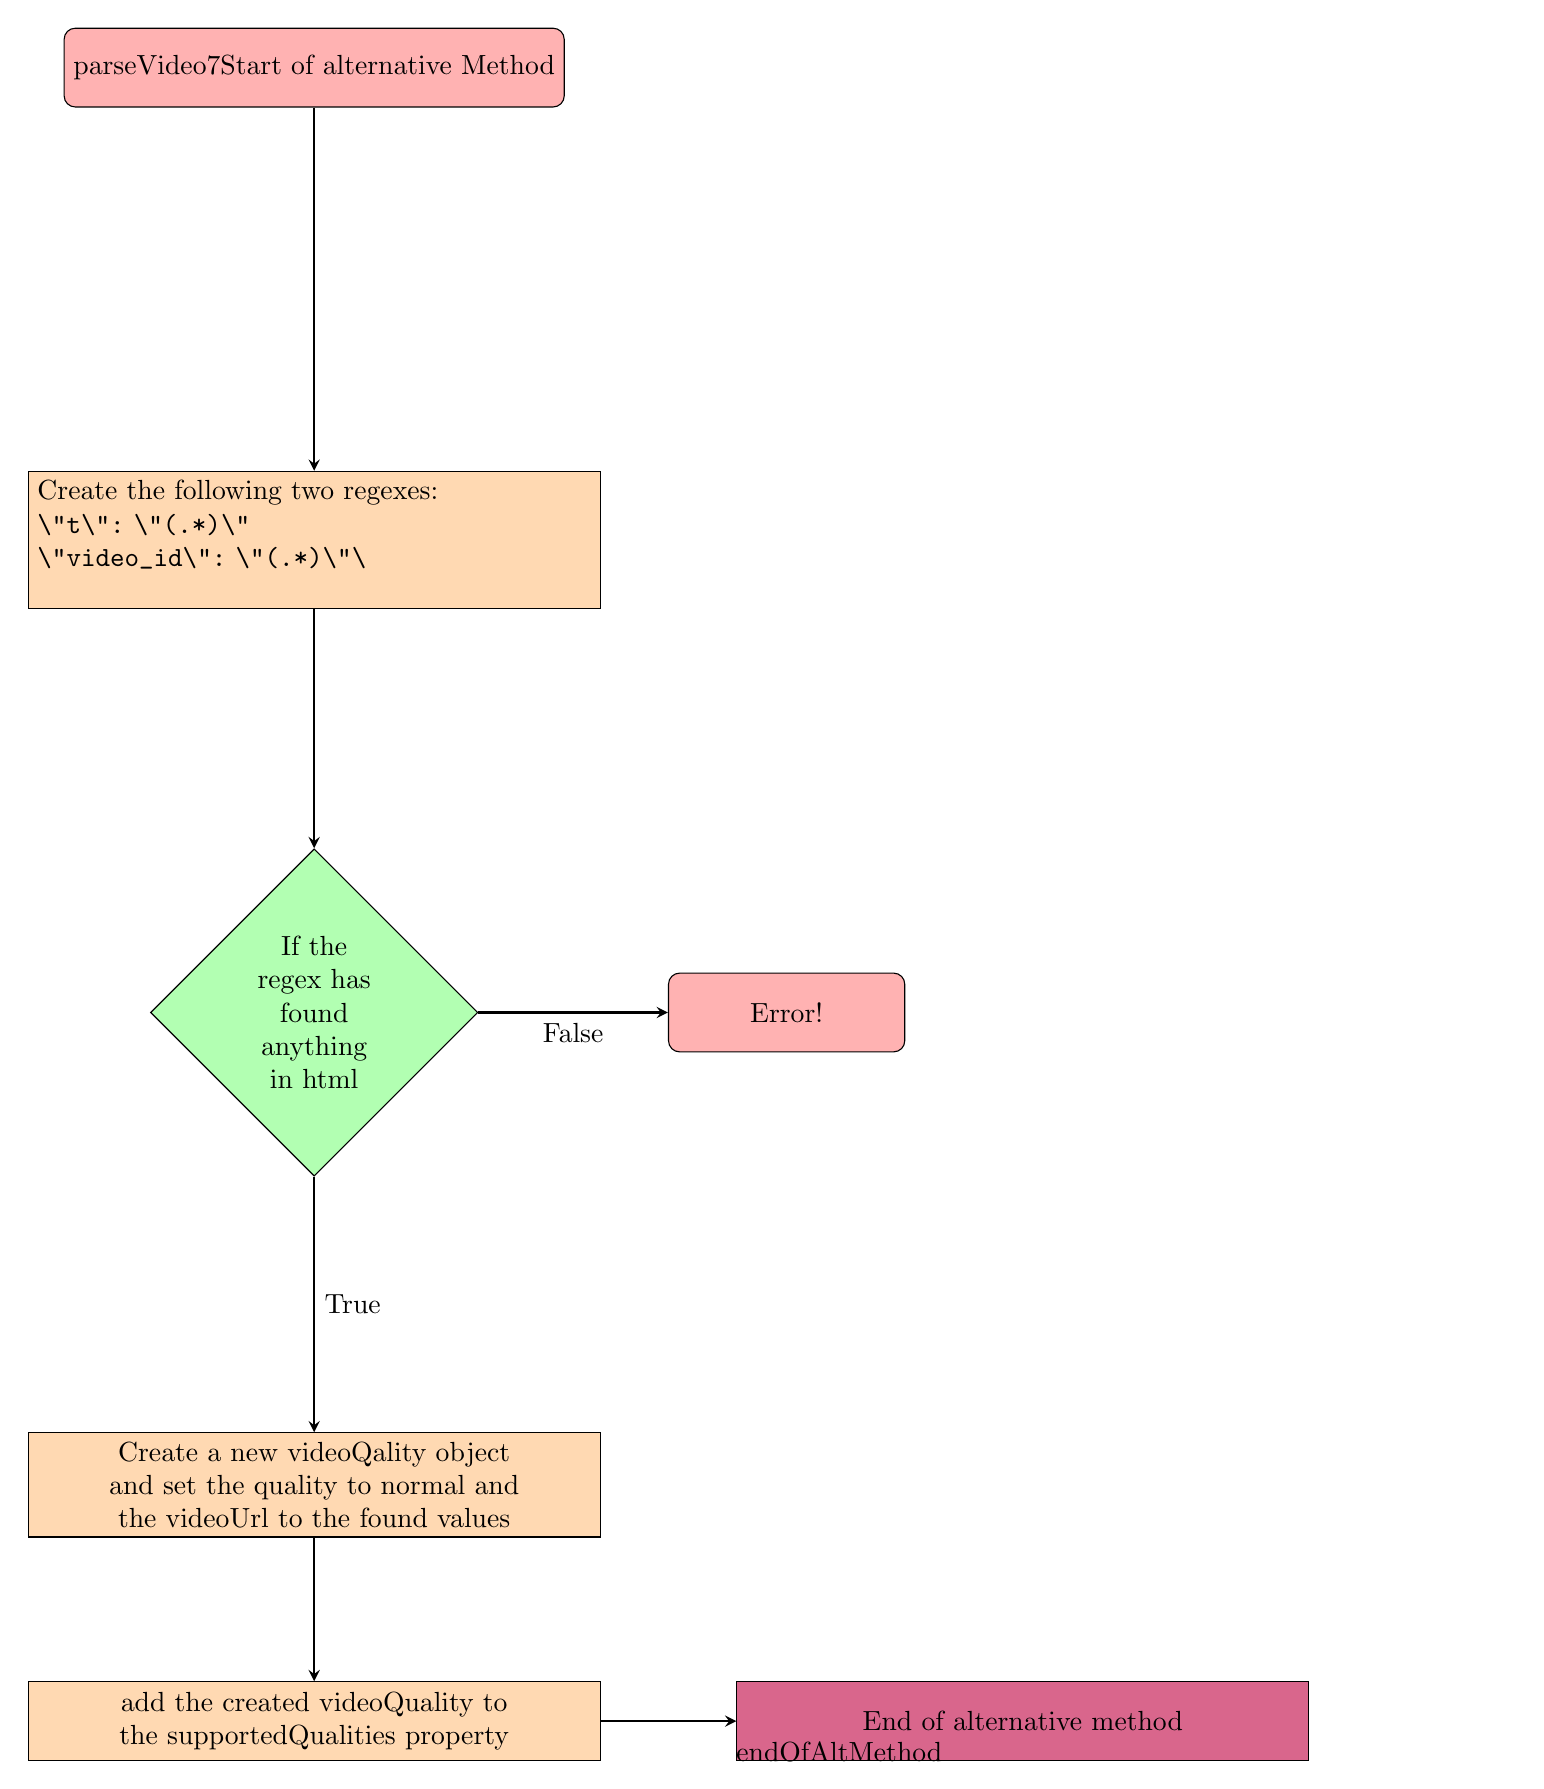
\begin{tikzpicture}[node distance=6cm]
        \node (start) [startstop] {\hypertarget{parseVideo7}{Start of alternative Method}};
        \node (regex) [process, below of=start] {Create the following two regexes:\newline
            \verb!\"t\": \"(.*)\"!\newline
            \verb!\"video_id\": \"(.*)\"\!\newline};
        \node (ifRegex) [decision, below of=regex] {If the regex has found anything in html};
        \node (error) [startstop, right of=ifRegex] {Error!};
        \node (initVideoQuality) [process, below of=ifRegex] {Create a new videoQality object and
            set the quality to normal and the videoUrl to the found values};
        \node (append) [process, yshift=3cm, below of=initVideoQuality] {add the created videoQuality to the
           supportedQualities property};
        \node (end) [process, xshift=3cm, hyperlink node=endOfAltMethod, fill=purple!60,
            right of=append] {End of alternative method};
        \draw [arrow] (start) -- node {} (regex);
        \draw [arrow] (regex) -- node {} (ifRegex);
        \draw [arrow] (ifRegex) -- node[anchor=west] {True} (initVideoQuality);
        \draw [arrow] (ifRegex) -- node[anchor=north] {False} (error);
        \draw [arrow] (initVideoQuality) -- node {} (append);
        \draw [arrow] (append) -- node {} (end);
    \end{tikzpicture}
\end{figure}
\begin{figure}[H]
    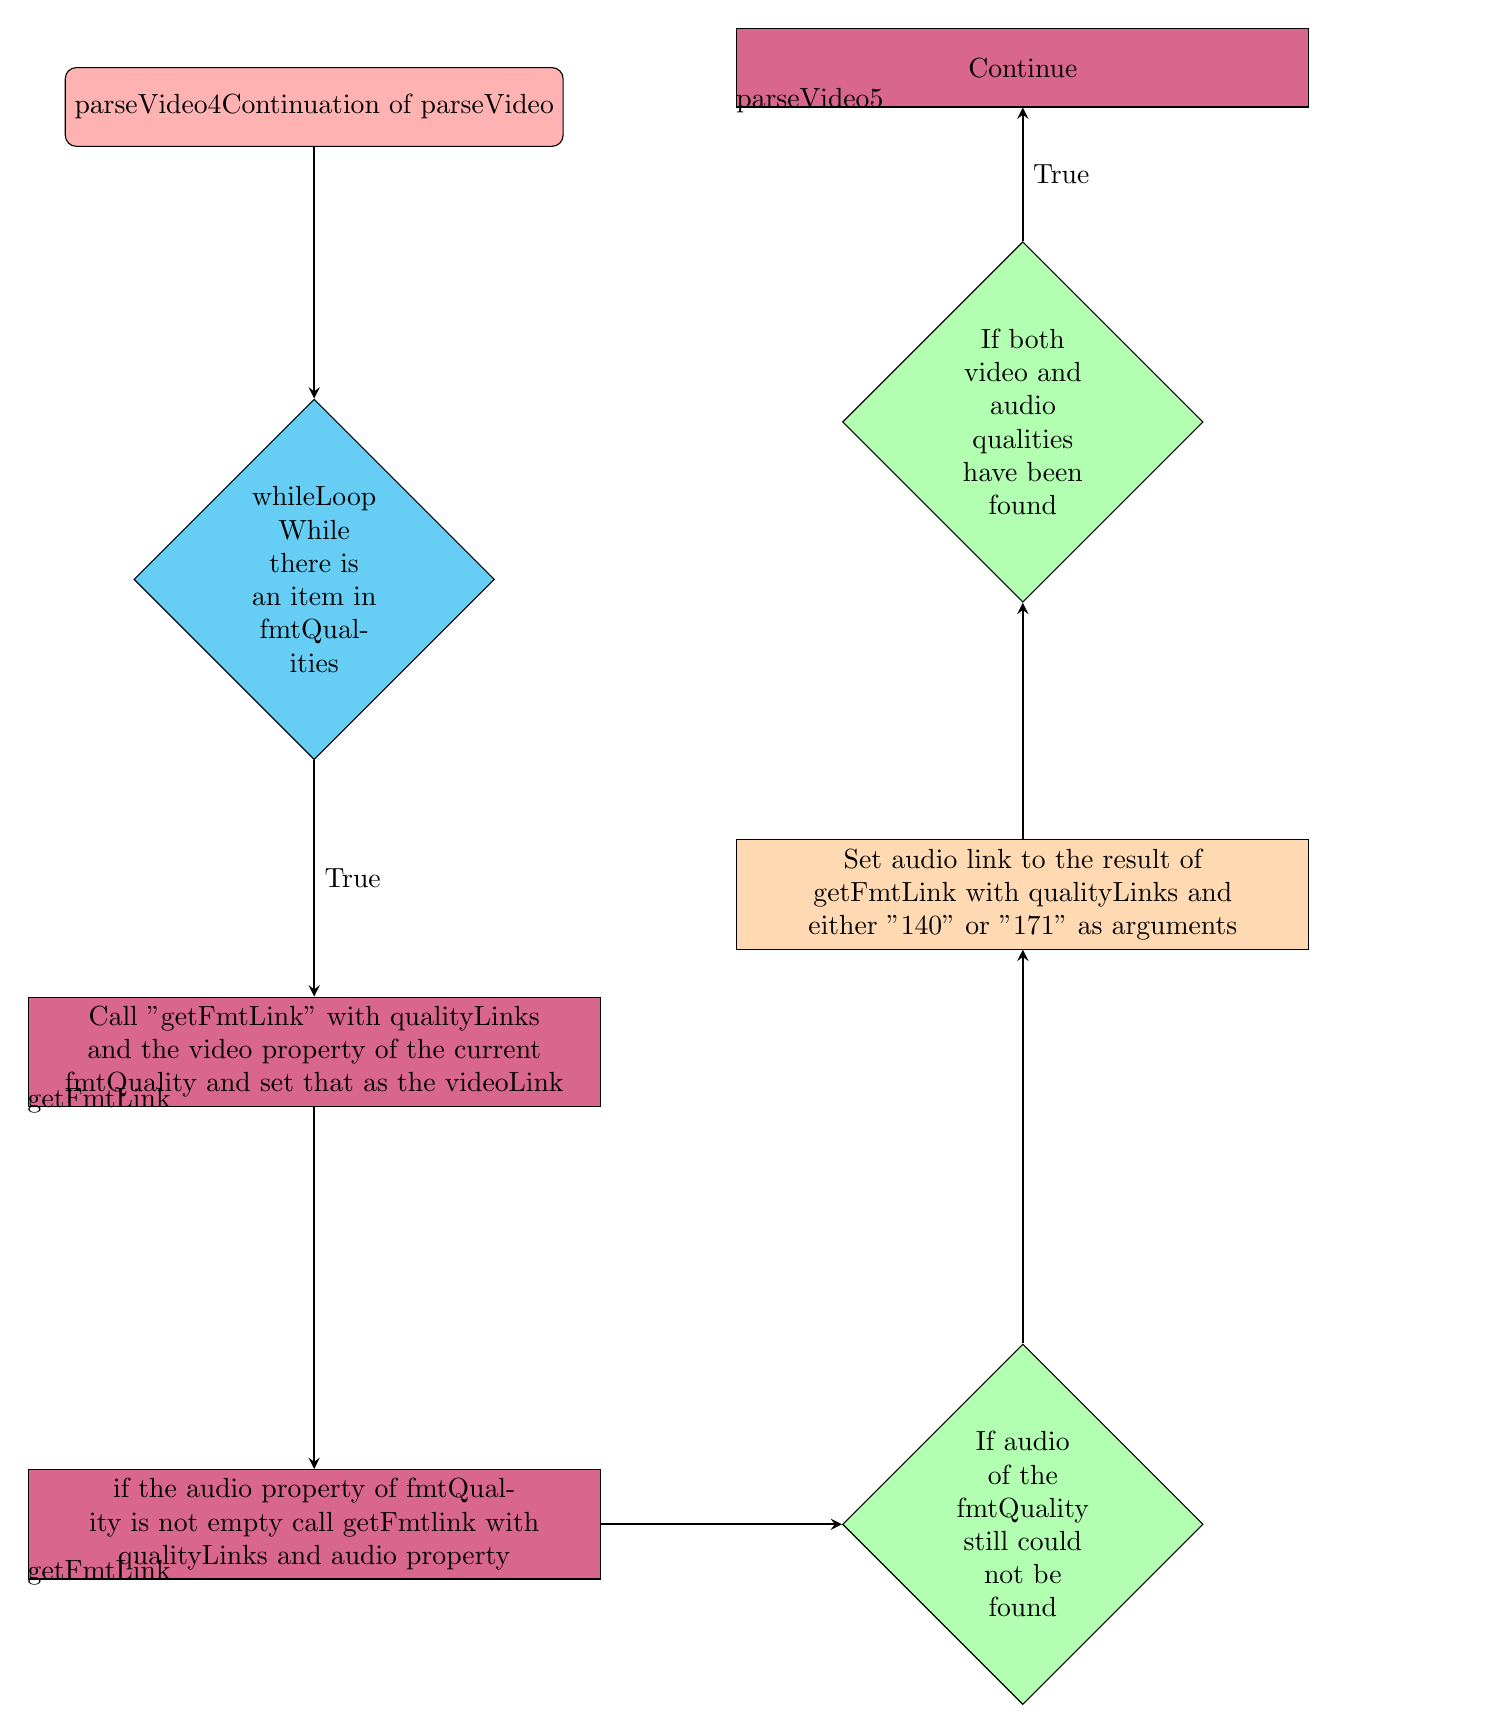
\begin{tikzpicture}[node distance=6cm]
        \node (start) [startstop] {\hypertarget{parseVideo4}{Continuation of parseVideo}};
        \node (whileLoop) [decision, fill=cyan!60, below of=start] {\hypertarget{whileLoop}
            {While there is an item in fmtQualities}};
        \node (createVideoLink) [process, hyperlink node=getFmtLink,
            fill=purple!60, below of=whileLoop] {Call "getFmtLink" with qualityLinks and
            the video property of the current fmtQuality and set that as the videoLink};
        \node (setAudioLink) [process, hyperlink node=getFmtLink,
            fill=purple!60, below of=createVideoLink] {if the audio property of fmtQuality is not
                empty call getFmtlink with qualityLinks and audio property};
        \node (ifAudioCouldNotBeFound) [decision, xshift=3cm, right of=setAudioLink] {If audio of
            the fmtQuality still could not be found};
        \node (manuallySetAudio) [process, yshift=2cm, above of=ifAudioCouldNotBeFound] {Set
            audio link to the result of getFmtLink with qualityLinks and either "140" or "171" as
            arguments};
        \node (ifQualityFound) [decision, above of=manuallySetAudio] {If both video and audio
            qualities have been found};
        \node (continue) [process, yshift=-1.5cm, hyperlink node=parseVideo5, fill=purple!60,
            above of=ifQualityFound] {Continue};
        \draw [arrow] (start) -- node {} (whileLoop);
        \draw [arrow] (whileLoop) -- node[anchor=west] {True} (createVideoLink);
        \draw [arrow] (createVideoLink) -- node {} (setAudioLink);
        \draw [arrow] (setAudioLink) -- node {} (ifAudioCouldNotBeFound);
        \draw [arrow] (ifAudioCouldNotBeFound) -- node {} (manuallySetAudio);
        \draw [arrow] (manuallySetAudio) -- node {} (ifQualityFound);
        \draw [arrow] (ifQualityFound) -- node[anchor=west] {True} (continue);
    \end{tikzpicture}
\end{figure}
\begin{figure}[H]
    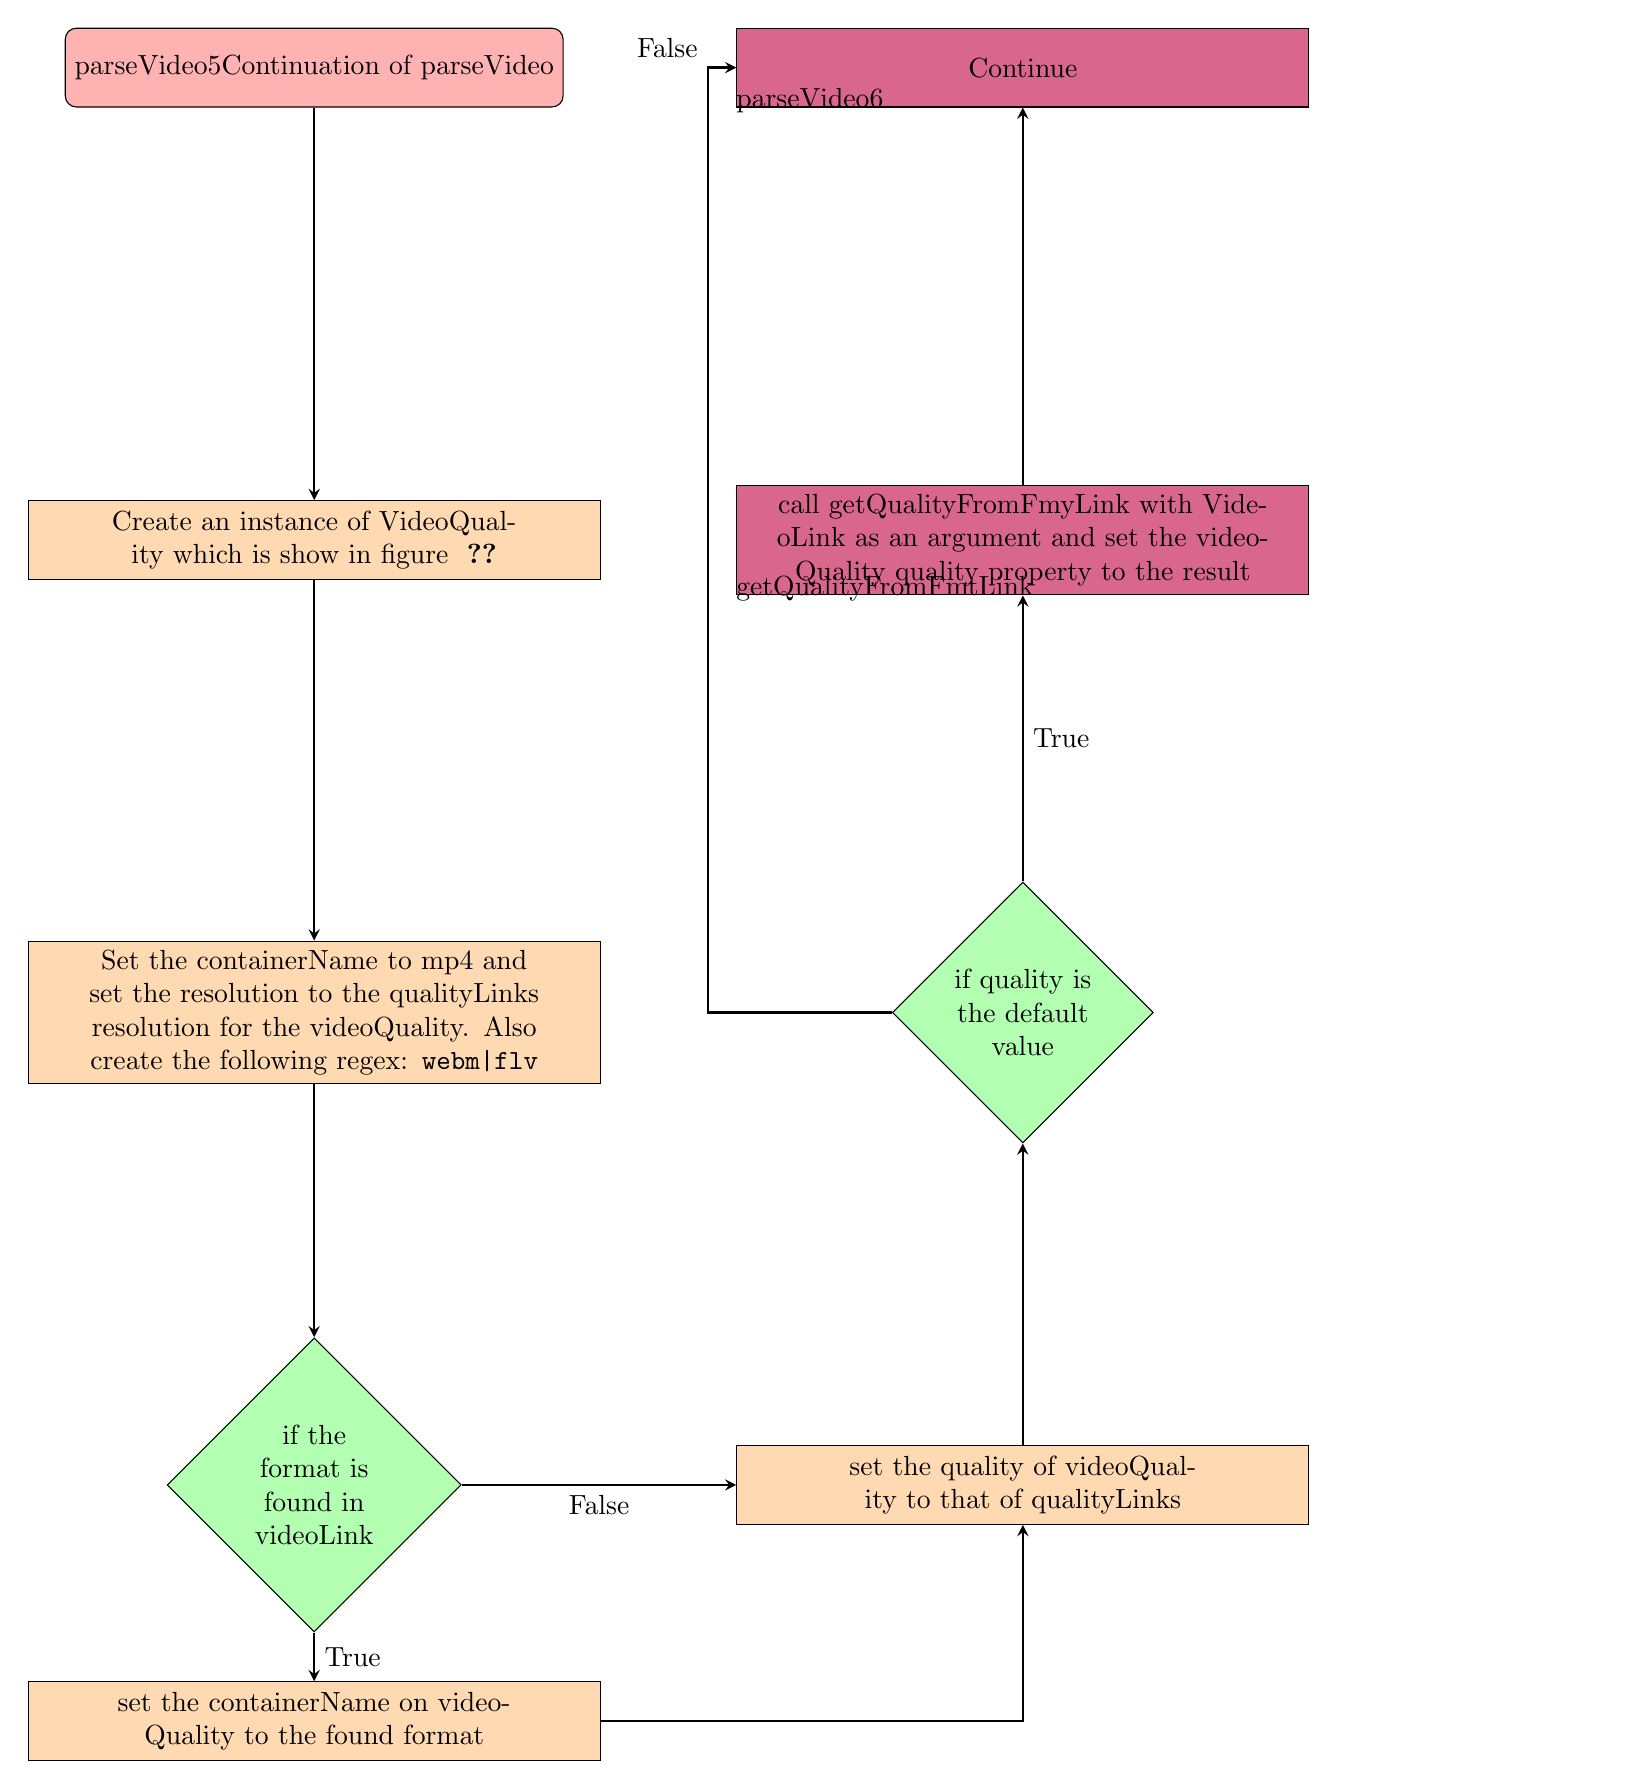
\begin{tikzpicture}[node distance=6cm]
        \node (start) [startstop] {\hypertarget{parseVideo5}{Continuation of parseVideo}};
        \node (initVideoQuality) [process, below of=start] {Create an instance of VideoQuality
            which is show in figure ~\ref{fig:Struct layout}};
        \node (createRegex) [process, below of=initVideoQuality] {Set the containerName to mp4
            and set the resolution to the qualityLinks resolution for the videoQuality.
            Also create the following regex: \verb!webm|flv!};
        \node (ifFoundContainer) [decision, below of=createRegex] {if the format is found in
            videoLink};
        \node (foundContainer) [process, yshift=3cm, below of=ifFoundContainer] {set the
            containerName on videoQuality to the found format};
        \node (setQuality) [process, xshift=3cm, right of=ifFoundContainer] {set the quality of
            videoQuality to that of qualityLinks};
        \node (ifQualityIsDefault) [decision, above of=setQuality] {if quality is the default
            value};
        \node (qualityIsDefault) [process, hyperlink node=getQualityFromFmtLink, fill=purple!60,
            above of=ifQualityIsDefault] {call getQualityFromFmyLink with VideoLink as an
            argument and set the videoQuality quality property to the result};
        \node (continue) [process, hyperlink node=parseVideo6, fill=purple!60,
            above of=qualityIsDefault] {Continue};
        \draw [arrow] (start) -- node {} (initVideoQuality);
        \draw [arrow] (initVideoQuality) -- node {} (createRegex);
        \draw [arrow] (createRegex) -- node {} (ifFoundContainer);
        \draw [arrow] (ifFoundContainer) -- node[anchor=west] {True} (foundContainer);
        \draw [arrow] (ifFoundContainer) -- node[anchor=north] {False} (setQuality);
        \draw [arrow] (foundContainer) -| node {} (setQuality);
        \draw [arrow] (setQuality) -- node {} (ifQualityIsDefault);
        \draw [arrow] (ifQualityIsDefault) -- node[anchor=west] {True} (qualityIsDefault);
        \draw [arrow] (qualityIsDefault) -- node {} (continue);
        \draw [arrow] (ifQualityIsDefault) -- +(-4,0) |- node[anchor=south east] {False}
            (continue);
    \end{tikzpicture}
\end{figure}
\begin{figure}[H]
    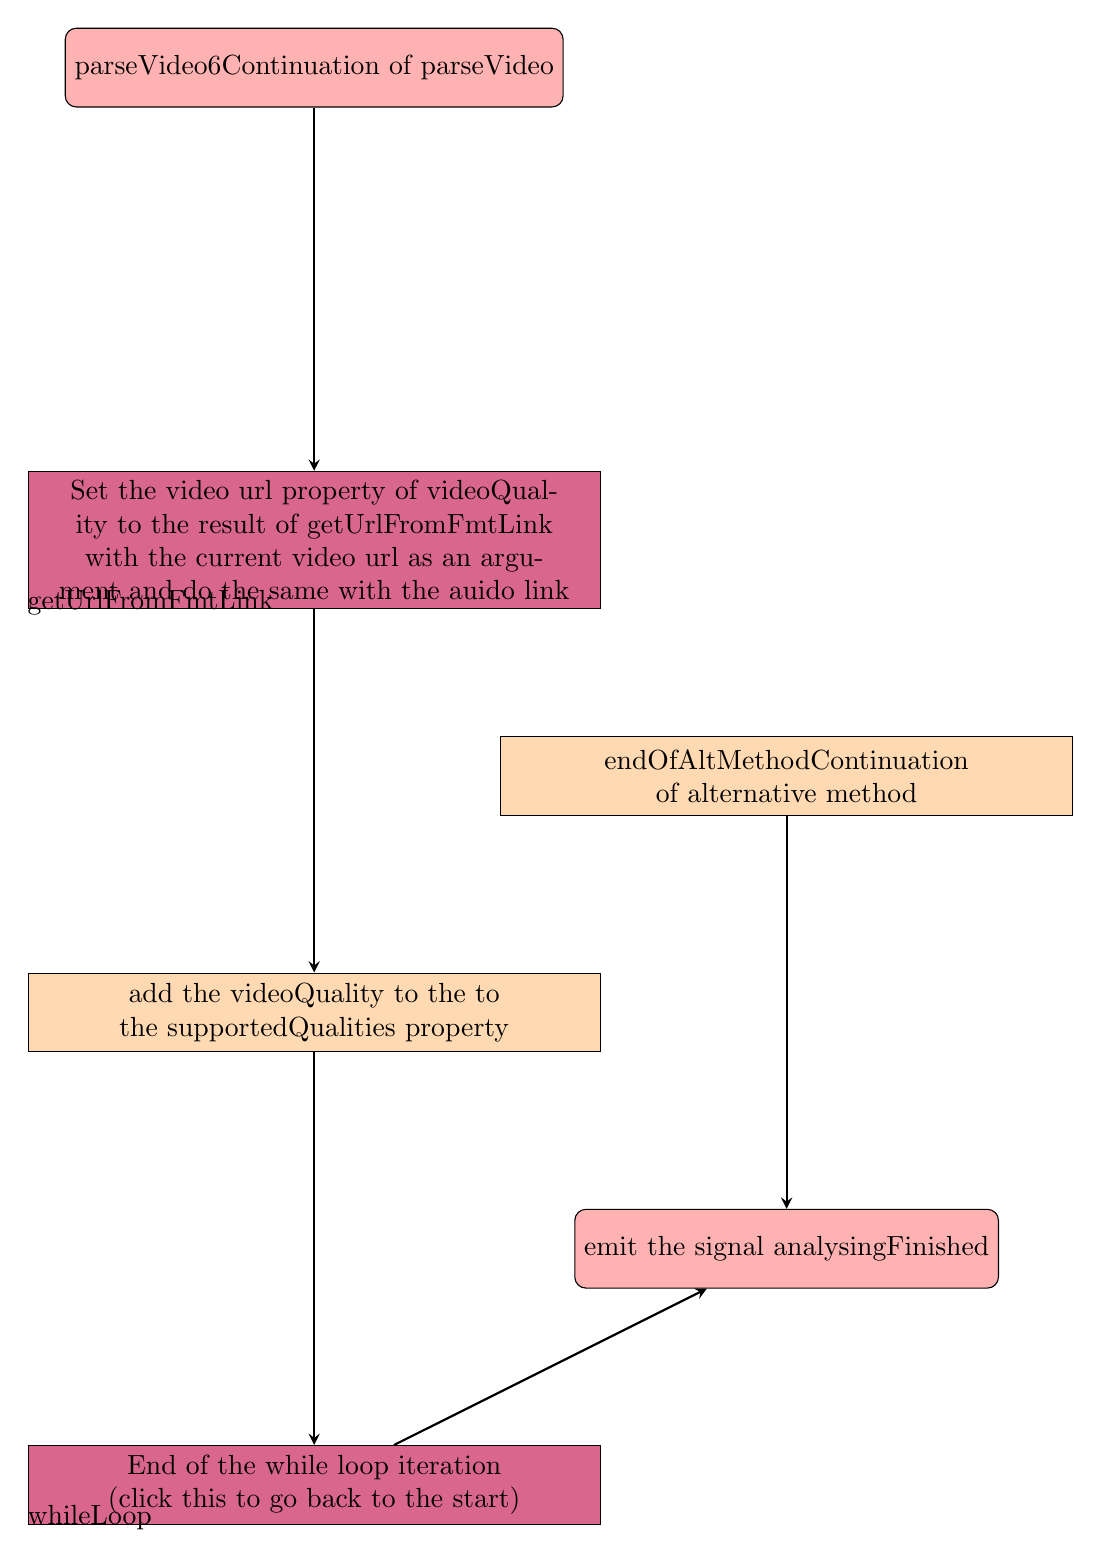
\begin{tikzpicture}[node distance=6cm]
        \node (start) [startstop] {\hypertarget{parseVideo6}{Continuation of parseVideo}};
        \node (setVideoUrl) [process, hyperlink node=getUrlFromFmtLink, fill=purple!60,
            below of=start] {Set the video url property of videoQuality to the result
            of getUrlFromFmtLink with the current video url as an argument and do the
            same with the auido link};
        \node (appendToSupportedQualities) [process, below of=setVideoUrl] {add the videoQuality
            to the to the supportedQualities property};
        \node (endOfWhileLoop) [process, hyperlink node=whileLoop, fill=purple!60,
            below of=appendToSupportedQualities] {End of the while loop iteration (click this
            to go back to the start)};
        \node (emitFinish) [startstop, yshift=3cm, right of=endOfWhileLoop] {emit the signal analysingFinished};
        \node (altMethod) [process, above of=emitFinish] {\hypertarget{endOfAltMethod}{Continuation of alternative method}};
        \draw [arrow] (start) -- node {} (setVideoUrl);
        \draw [arrow] (setVideoUrl) -- node {} (appendToSupportedQualities);
        \draw [arrow] (appendToSupportedQualities) -- node {} (endOfWhileLoop);
        \draw [arrow] (endOfWhileLoop) -- node {} (emitFinish);
        \draw [arrow] (altMethod) -- node {} (emitFinish);
    \end{tikzpicture}
\end{figure}
\begin{figure}[H]
    \begin{tikzpicture}[node distance=6cm]
        \node (start) [startstop] {\hypertarget{getUrlFromFmtLink}{start of
            getQualityFromFmtLink}};
        \node (regex1) [process, below of=start] {Create two regular expression: urlExpression
            and sigExpression which are respectively:\newline
            \verb!(http[s]?[^,]+)!\newline
            \verb!(?:^|[^a-zA-Z])[,]?s(ig)?=([^,]+)!\newline};
        \node (extractUrl) [process, below of=regex] {Extract the url and signature
            from the link parameter};
        \node (checkSig) [process, hyperlink node=parseSignature, fill=purple!60,
            below of=extractUrl] {if the signature does not equal "ig" then call parseSignature
            with signature as a argument};
        \node (return) [startstop, yshift=-3cm, xshift=-3cm, above right =of checkSig] {append the signature to url and return
            the url};
        \draw [arrow] (start) -- node {} (regex1);
        \draw [arrow] (regex1) -- node {} (extractUrl);
        \draw [arrow] (extractUrl) -- node {} (checkSig);
        \draw [arrow] (checkSig) -| node {} (return);
    \end{tikzpicture}
\end{figure}
\begin{figure}[H]
    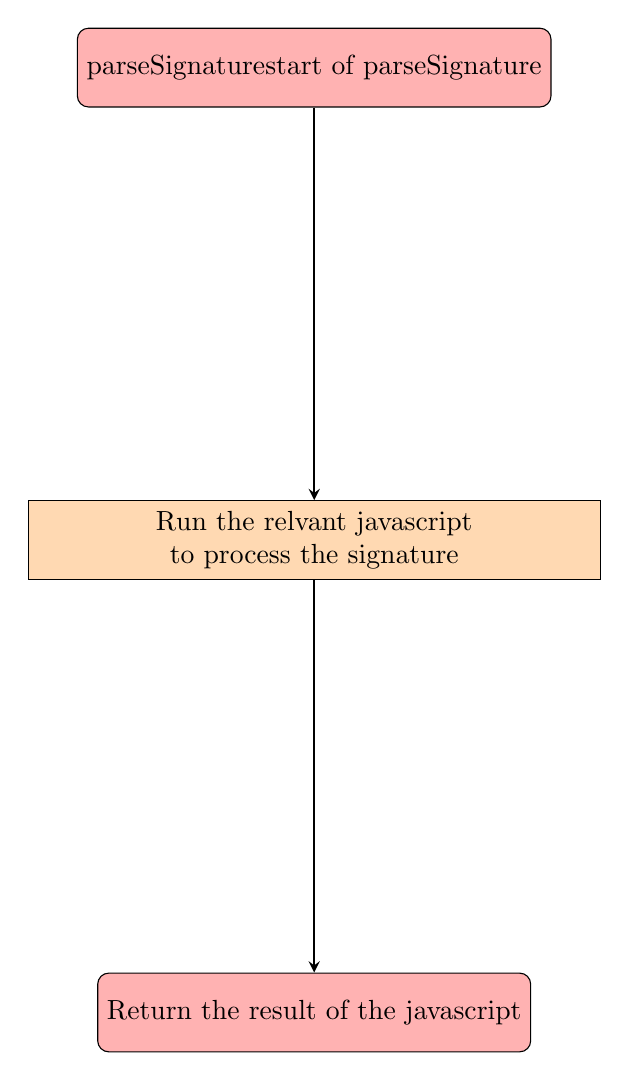
\begin{tikzpicture}[node distance=6cm]
        \node (start) [startstop] {\hypertarget{parseSignature}{start of parseSignature}};
        \node (runJs) [process, below of=start] {Run the relvant javascript to process the signature};
        \node (return) [startstop, below of=runJs] {Return the result of the javascript};
        \draw [arrow] (start) -- node {} (runJs);
        \draw [arrow] (runJs) -- node {} (return);
    \end{tikzpicture}
\end{figure}
\begin{figure}[H]
    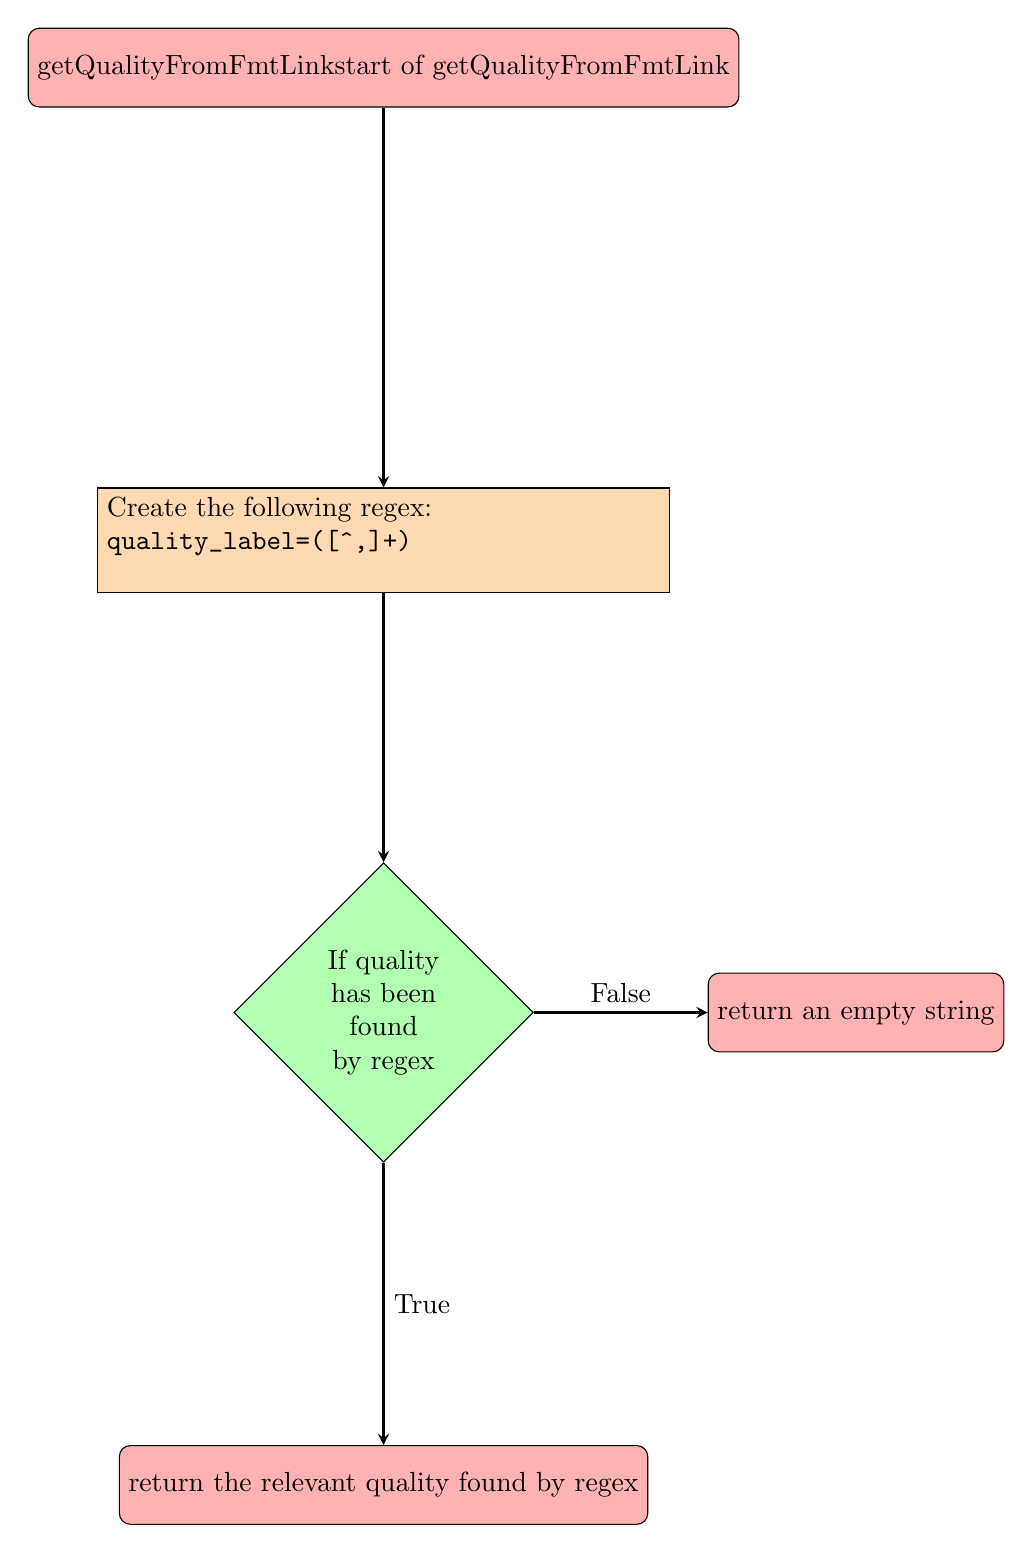
\begin{tikzpicture}[node distance=6cm]
        \node (start) [startstop] {\hypertarget{getQualityFromFmtLink}{start of
            getQualityFromFmtLink}};
        \node (regex) [process, below of=start] {Create the following regex:\newline
           \verb!quality_label=([^,]+)!\newline};
        \node (ifFound) [decision, below of=regex] {If quality has been found by regex};
        \node (foundTrue) [startstop, below of=ifFound] {return the relevant quality found by regex};
        \node (foundFalse) [startstop, right of=ifFound] {return an empty string};
        \draw [arrow] (start) -- node {} (regex);
        \draw [arrow] (regex) -- node {} (ifFound);
        \draw [arrow] (ifFound) -- node[anchor=west] {True} (foundTrue);
        \draw [arrow] (ifFound) -- node[anchor=south] {False} (foundFalse);
    \end{tikzpicture}
\end{figure}
\begin{figure}[H]
    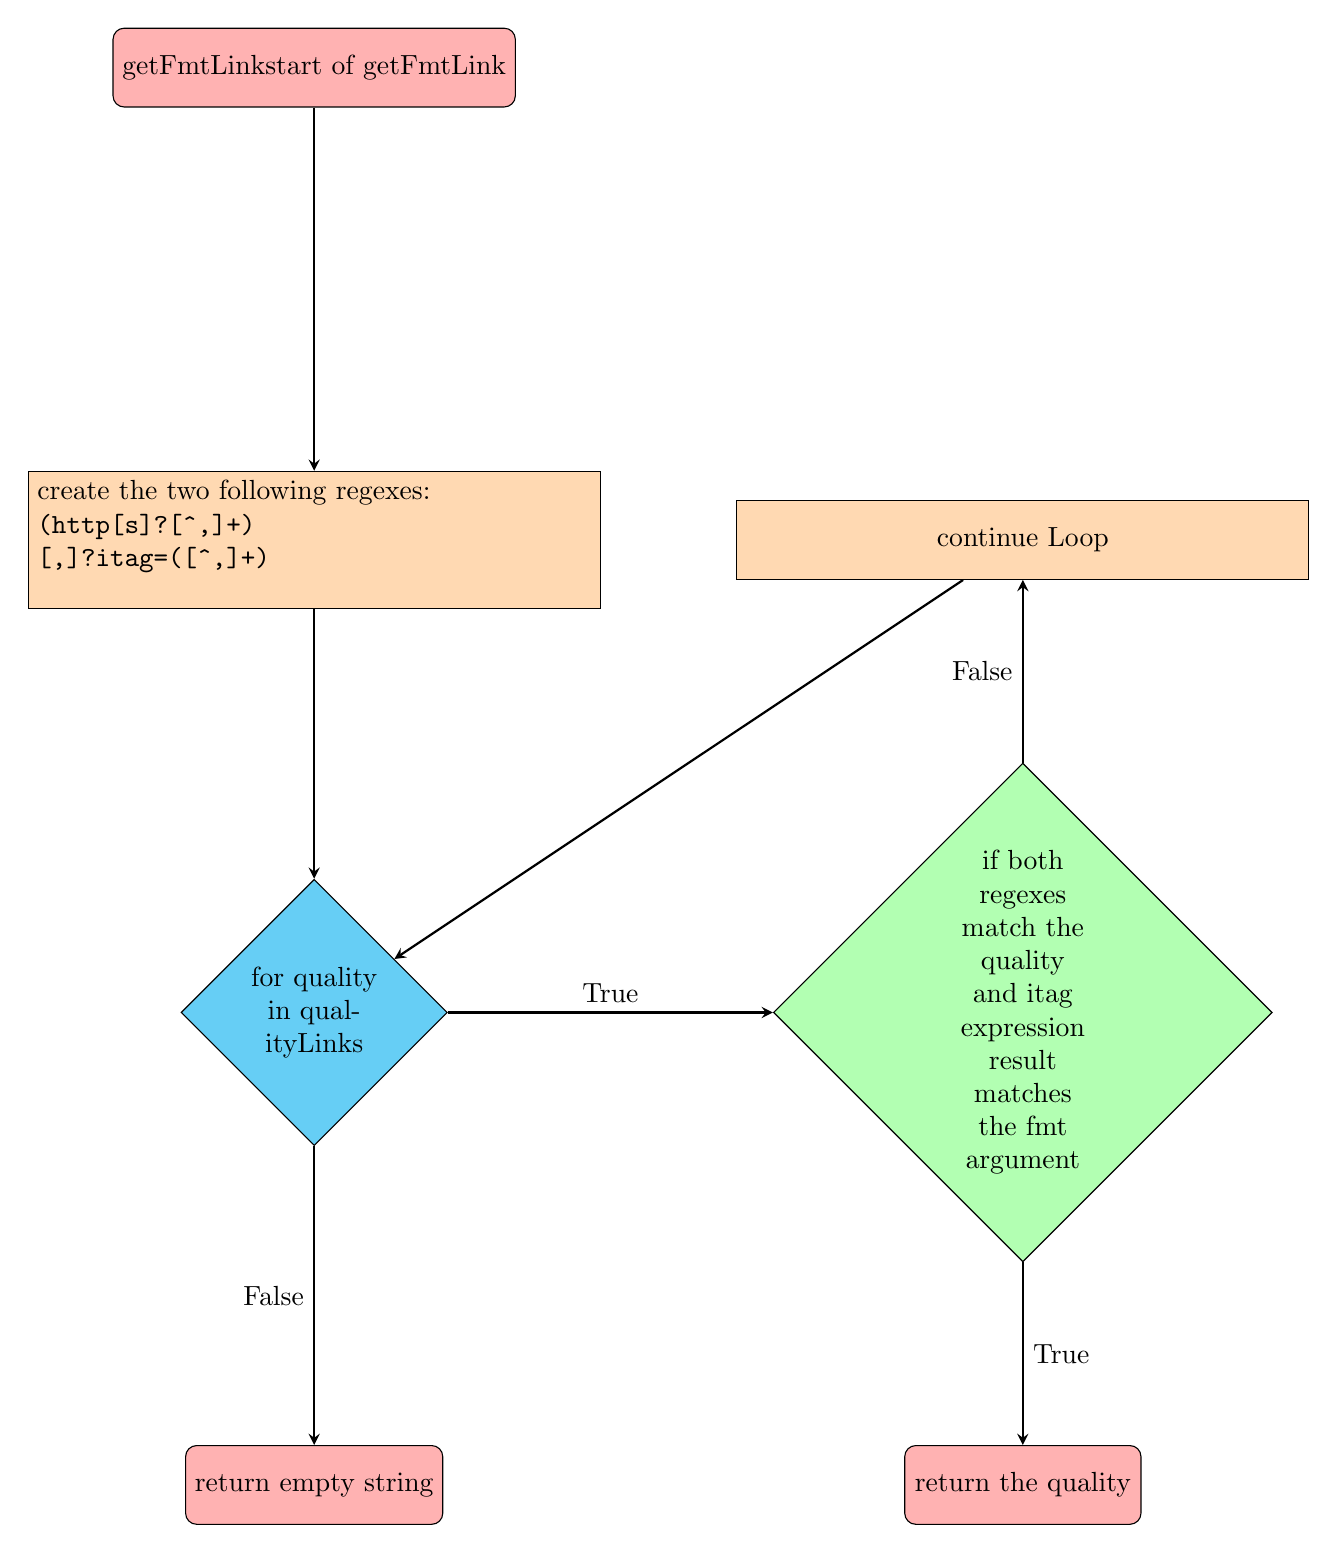
\begin{tikzpicture}[node distance=6cm]
        \node (start) [startstop] {\hypertarget{getFmtLink}{start of getFmtLink}};
        \node (regex) [process, below of=start] {create the two following regexes:\newline
            \verb!(http[s]?[^,]+)!\newline
            \verb![,]?itag=([^,]+)!\newline};
        \node (forLoop) [decision, fill=cyan!60, below of=regex] {for quality in qualityLinks};
        \node (ifFound) [decision, xshift=3cm, right of=forLoop] {if both regexes match the quality and itag
            expression result matches the fmt argument};
        \node (foundTrue) [startstop, below of=ifFound] {return the quality};
        \node (foundFalse) [process, above of=ifFound] {continue Loop};
        \node (return) [startstop, minimum width=1cm, below of=forLoop] {return empty string};
        \draw [arrow] (start) -- node {} (regex);
        \draw [arrow] (regex) -- node {} (forLoop);
        \draw [arrow] (forLoop) -- node[anchor=south] {True} (ifFound);
        \draw [arrow] (ifFound) -- node[anchor=west] {True} (foundTrue);
        \draw [arrow] (ifFound) -- node[anchor=east] {False} (foundFalse);
        \draw [arrow] (foundFalse) -- node[anchor=east] {} (forLoop);
        \draw [arrow] (forLoop) -- node[anchor=east] {False} (return);
    \end{tikzpicture}
\end{figure}
\begin{figure}[H]
    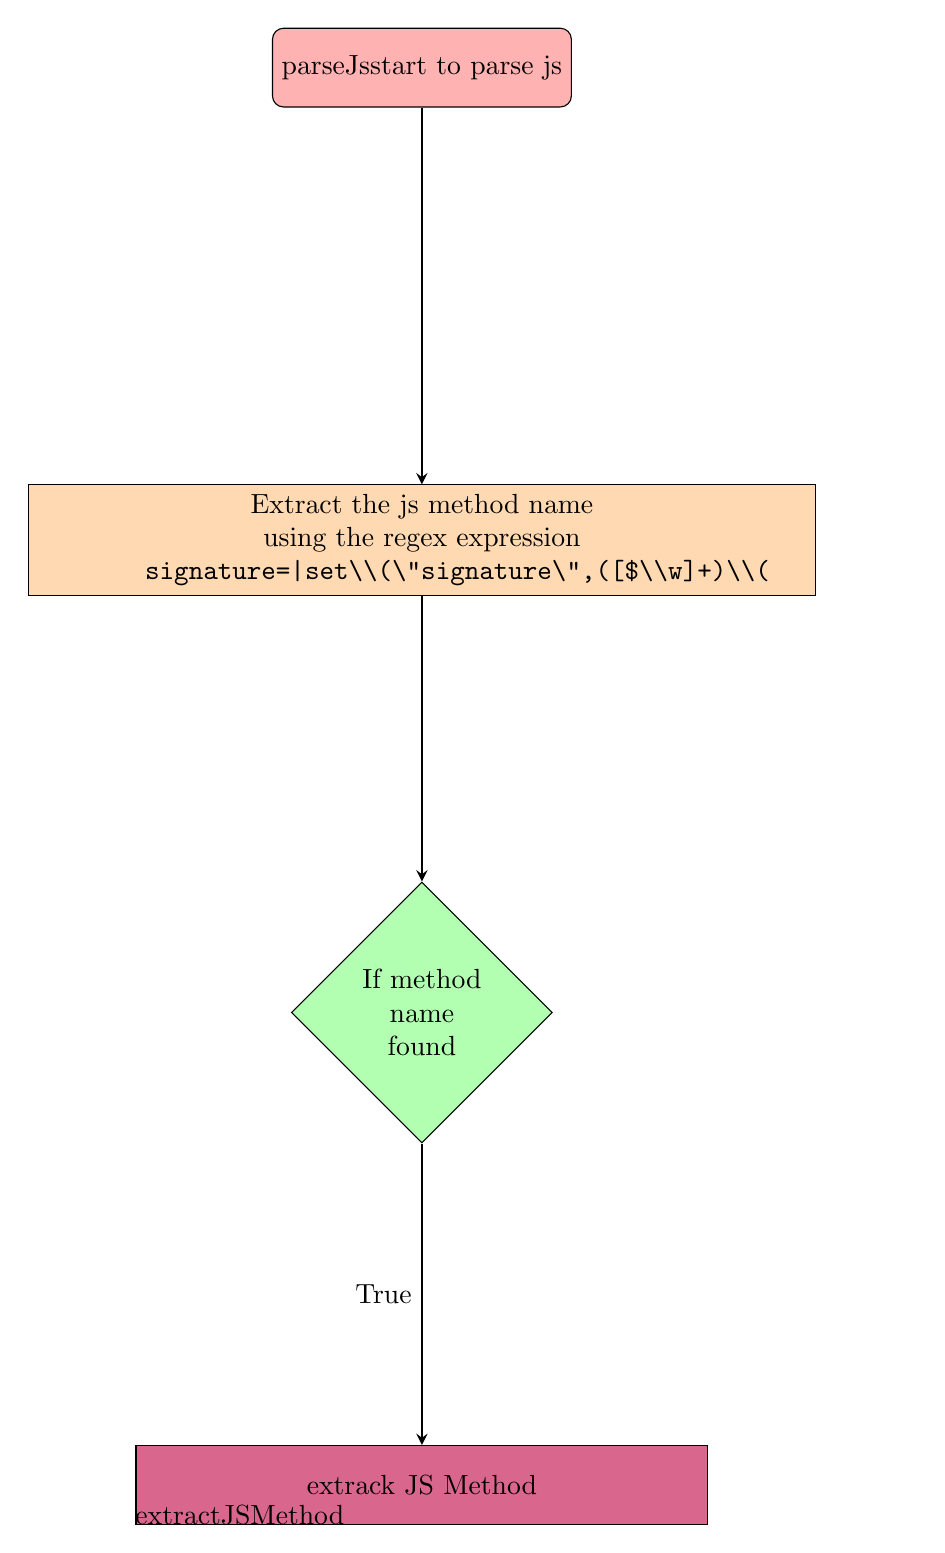
\begin{tikzpicture}[node distance=6cm]
        \node (start) [startstop] {\hypertarget{parseJs}{start to parse js}};
        \node (regexExpression) [process, below of=start, minimum width=10cm] {
                Extract the js method name using the regex expression
                \verb!signature=|set\\(\"signature\",([$\\w]+)\\(!
            };
        \node (ifFound) [decision, below of=regexExpression] {If method name found};
        \node (methodCall) [process, fill=purple!60, hyperlink node=extractJSMethod, below of=ifFound] {extrack JS Method};
        \draw [arrow] (start) -- node {} (regexExpression);
        \draw [arrow] (regexExpression) -- node {} (ifFound);
        \draw [arrow] (ifFound) -- node[anchor=east] {True} (methodCall);
    \end{tikzpicture}
\end{figure}
\begin{figure}[H]
    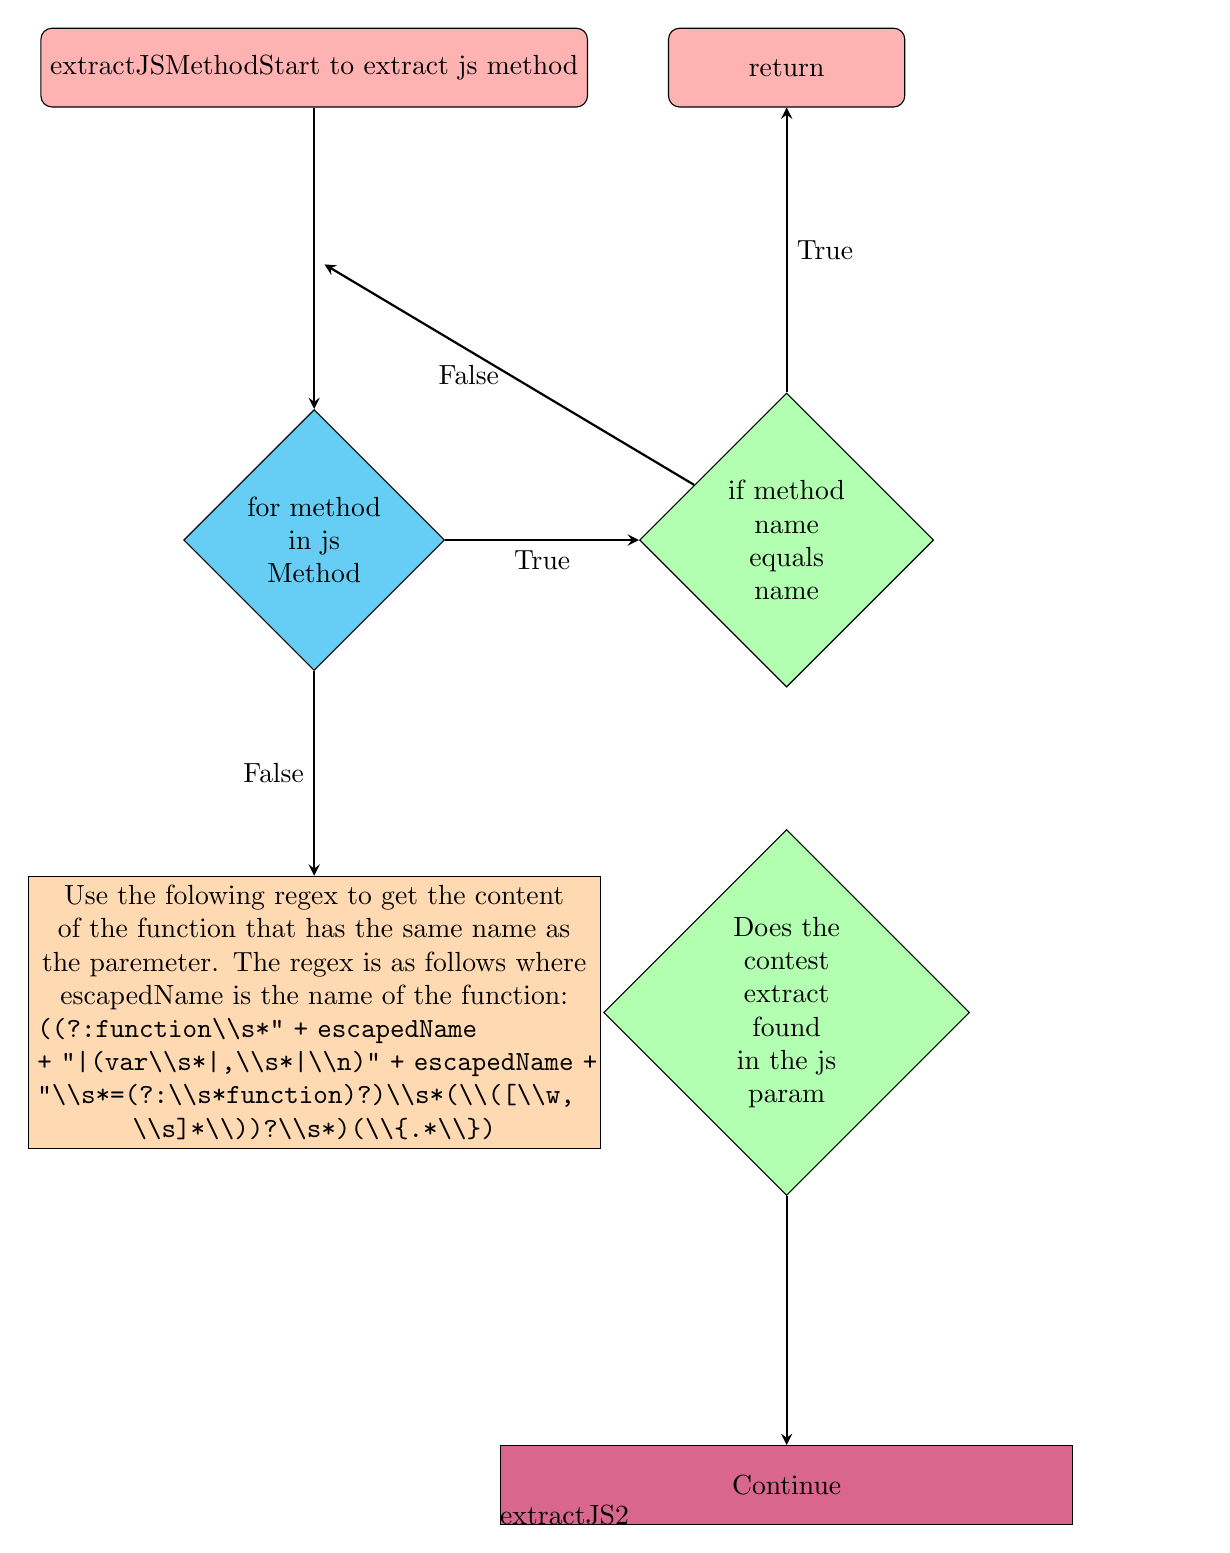
\begin{tikzpicture}[node distance=6cm]
        \node (start) [startstop] {\hypertarget{extractJSMethod}{Start to extract js method}};
        \node (checkIfCompleted) [decision, fill=cyan!60, below of=start] {for method in js
            Method};
        \node (ifComplete) [decision, right of=checkIfCompleted] {if method name equals name};
        \node (isCompleted) [startstop, above of=ifComplete] {return};
        \draw [arrow] (start) -- node (CheckCompleteforarrow) {} (checkIfCompleted);
        \draw [arrow] (checkIfCompleted) -- node[anchor=north] {True} (ifComplete);
        \draw [arrow] (ifComplete) -- node[anchor=west] {True} (isCompleted);
        \draw [arrow] (ifComplete) -- node[anchor=east] {False} (CheckCompleteforarrow);
        \node (firstFunctionRegex) [process, below of=checkIfCompleted] {Use the folowing regex to get the content
        of the function that has the same name as the paremeter. The regex is as follows where escapedName is the
        name of the function:
        \verb!((?:function\\s*" + escapedName!\newline
        \verb!+ "|(var\\s*|,\\s*|\\n)" + escapedName +!\newline
        \verb!"\\s*=(?:\\s*function)?)\\s*(\\([\\w,!\newline
        \verb!\\s]*\\))?\\s*)(\\{.*\\})!};
        \draw [arrow] (checkIfCompleted) -- node[anchor=east] {False} (firstFunctionRegex);
        \node (checkIfContentMatchParam) [decision, right of=firstFunctionRegex] {Does the contest extract found in the js param};
        \node (extractJsContinued) [process, hyperlink node=extractJS2, fill=purple!60, below of=checkIfContentMatchParam] {Continue};
        \draw [arrow] (checkIfContentMatchParam) -- node {} (extractJsContinued);
    \end{tikzpicture}
\end{figure}
\begin{figure}[H]
    \begin{tikzpicture}[node distance=6cm]
        \node (start) [startstop] {\hypertarget{extractJS2}{extractJS method part 2}};
        \node (createObject) [process, below of=start] {Initializes a object of type jsMethod (Fig ~\ref{fig:Struct layout})};
        \node (setProperties) [process, below of=createObject] {Set the name, code properties of jsMethod and add to jsMethods
                                                                property};
        \node (ifMethodCodeNotEmpty) [decision, right of=setProperties] {Is the object code empty};
        \node (regex) [process, above of=ifMethodCodeNotEmpty, yshift=-1.5cm] {Use the follow regex:
            \verb!([\\w\\$]+)(?:[\\w\\.\\$])*\\s*!\newline
            \verb!(\\([\\w\\s,\"\\$]*)\\)!};
        \node (recursive) [process, above of=regex, yshift=-1.5cm] {The regex should find functions called inside. After finding these functions
        call \hypertarget{extractJSMethod}{extractJS} with the name and code as arguments};
        \node (stop) [startstop, above of=recursive] {Finish};
        \draw [arrow] (start) -- node {} (createObject);
        \draw [arrow] (createObject) -- node {} (setProperties);
        \draw [arrow] (setProperties) -- node {} (ifMethodCodeNotEmpty);
        \draw [arrow] (ifMethodCodeNotEmpty) -- node[anchor=east] {False} (regex);
        \draw [arrow] (regex) -- node {} (recursive);
        \draw [arrow] (recursive) -- node {} (stop);
        \node (escapeRegex) [process, below of=checkIfCompleted] {Find the contents of the
            method from the name using a regular expression};
    \end{tikzpicture}
\end{figure}
\pagebreak
\subsection{Burning the audio CD}
Due to one of my original requirements I need to ensure that this program is cross-platform
which raises a problem when it comes to the cd burning process as different platforms have
different methods to burning an audio data to a cd. To resolve this problem I decide that
I would run 3rd party software that would be able to run on all platforms from my own
program. There are a few out there but the one that seemed best supported and had good
documentation was the cdrtools collection. The program in this collection that is relevent
to this project is "cdrecord". This program allows data to be burnt to a cd of your choosing.
unfortunately running this within the program normally will cause it to freeze until it finishes.
Because of this I think it will be best to use another thread to run this process in. Luckily
Qt has a class call QThread which allow threading in qt.
I was also unsure whether the program could be called multiple times with a different track
and CD as this would be the best approach to burning music to the cds for two reasons. The
first is that if there is an error burning one track the others should still be able be burnt
onto the cd. The second is that I can update the progress bar with each succesful burning operation.
I thought the best way for me to figure this out was to test the executable with various options.
After testing the cdrecord program, I found that the following arguments are required to perform the
desired behaviour: -dev, -pad, -multi and -tao. The dev option is use to set the id of the
cd drive you wish to use. You can find out this device id by running the program with the -scanbus
option. unfortunately on Linux this does required root permission, when I tried using it with a
usb cd, which generally is a bad idea and could cause problems in other areas of my program. The
only solution to this permission issue is to edit the sudoers file to make an exception for this
command. The next option, -pad, is used to make the audio data from the downloaded file a multiple
of 2352 bytes. This is a required standard for audio CDs. the "-multi" option does exactly what
I want to do in regards to burning each track in separate commands. Finally the "-tao" option is
actually something that is enabled by default by cdrecord but by explicitly specifying the option
it will speed up the execution process by not doing a count down.
\subsection{Data flow and data types}
In this section I will define all of the data requirements for this project which will include
the information imputed by the user and the final output. The database and the converted audio
files are all stored in the downloads folder. This is a directory created by the DataHandler
class where it create a new folder from the builds current path called downloads. Before being
converted the audio data is saved in the temporary folder of the current OS it is running on.
For example on Linux this is "/tmp". The reasoning behind this is that the download may get
interrupted and become corrupted making it difficult to deal with. If it save in the temporary
folder the OS deals with it automatically and will clean up any mess left.
\subsubsection{Data diagram}
\begin{figure}[H]
    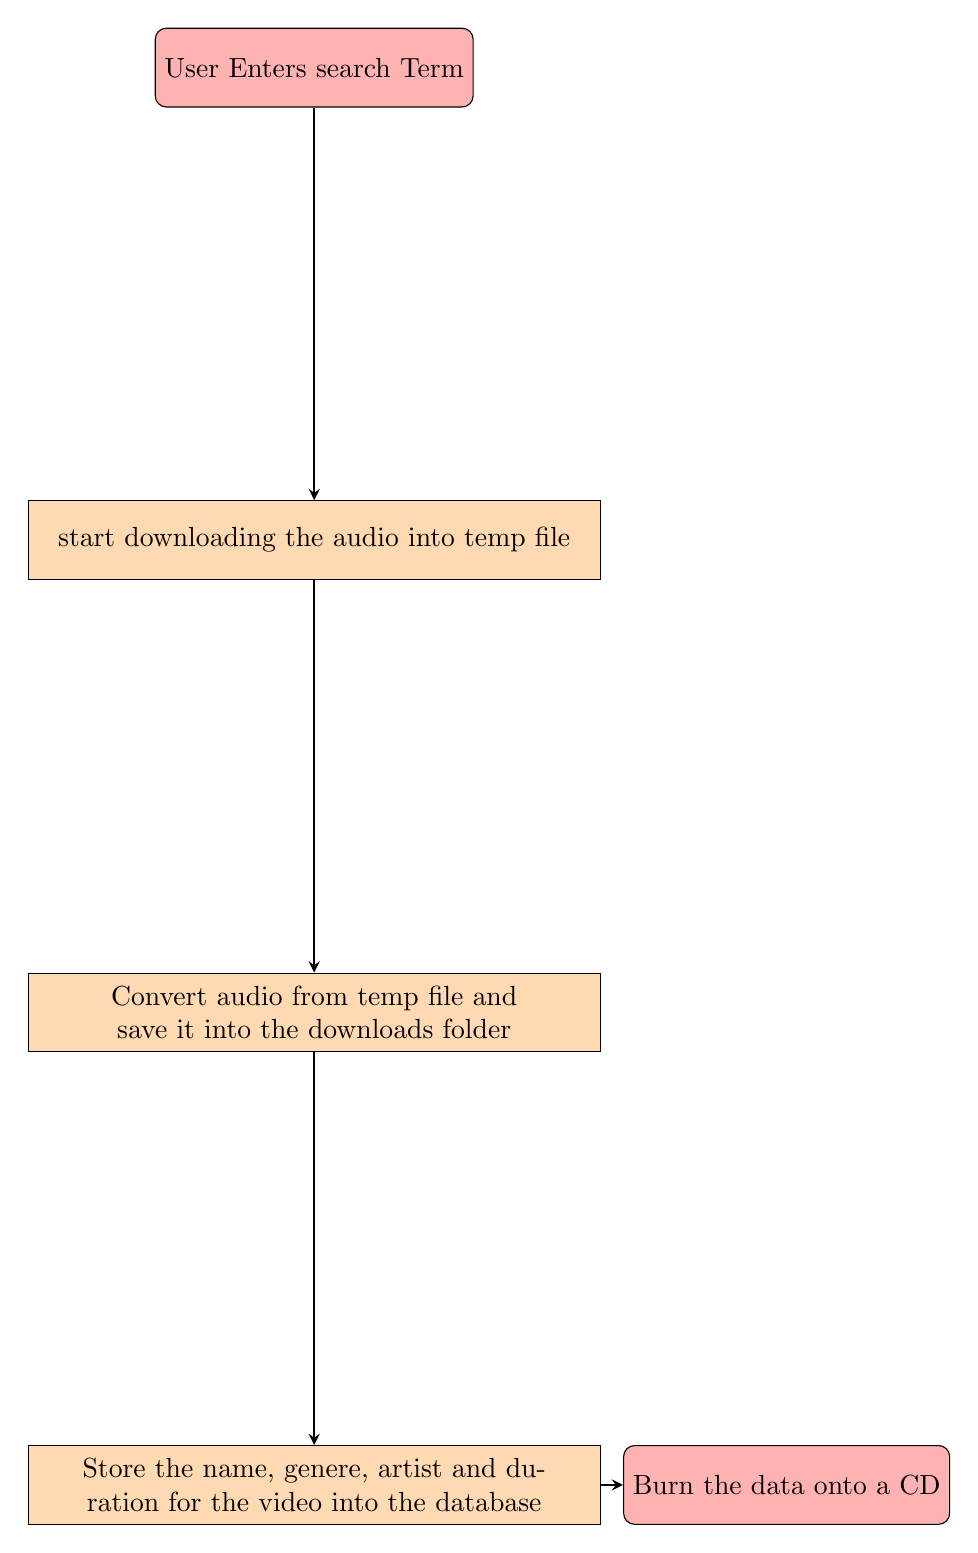
\begin{tikzpicture}[node distance=6cm]
        \node (start) [startstop] {User Enters search Term};
        \node (downloadTemp) [process, below of=start] {start downloading the audio into temp file};
        \node (convert) [process, below of=downloadTemp] {Convert audio from temp file and save it
            into the downloads folder};
        \node (database) [process, below of=convert] {Store the name, genere, artist and duration
            for the video into the database};
        \node (burn) [startstop, right of=database] {Burn the data onto a CD};
        \draw [arrow] (start) -- node {} (downloadTemp);
        \draw [arrow] (downloadTemp) -- node {} (convert);
        \draw [arrow] (convert) -- node {} (database);
        \draw [arrow] (database) -- node {} (burn);
    \end{tikzpicture}
    \caption{Data flow diagram} \label{fig:Data flow diagram}
    This diagram illustrates the basic data flow of the application.
\end{figure}
\subsubsection{Data Structures used}
There are many data structures that are introduced by the qt framework. You can usually distinguish
these data structures from the normal c++ data structures by the fact they have a "Q" affixed to
the start of their name. These data structures are described in figure ~\ref{fig:qtDataStructs}.
\begin{figure}[H]
    \begin{center}
        \begin{tabular} {| c | c |}
            \hline
            \textbf{Name}        &         \textbf{Desciption}                               \\ \hline
            QString              &This acts the same as a normal string type but has methods \\
                                 &that help interaction with it. These methods are described  \\
                                 &\href{https://doc.qt.io/qt-5/qstring.html}{here}           \\ \hline
            QList                &This acts the same as a normal list but has additional     \\
                                 &properties and methods to interact with it. You can find   \\
                                 &more information about these extended features             \\
                                 &\href{https://doc.qt.io/qt-5/qlist.html}{here}             \\ \hline
            QHash                &This is a hash table type that you can use like a          \\
                                 &dictionary/map. There is a similar Qt data structure called\\
                                 &QMap but this type has a higher algorithmic complexity     \\
                                 &making it slower that QHash. Because of this I have only   \\
                                 &used the QHash type and not QMap. You can find more        \\
                                 &information \href{https://doc.qt.io/qt-5/qhash.html}{here} \\ \hline
            QStringList          &This is a type derived from QList and is design to only    \\
                                 &house QStrings and nothing else. More information can be   \\
                                 &\href{http://doc.qt.io/qt-5/qstringlist.html}{here}        \\ \hline
            qint64               &This is an integer type that have 64 bytes of memory      \\
                                 &allocated to it. This will likely only be used for the     \\
                                 &progress bars and nothing else. Data about this type can be\\
                                 &found                                                      \\
                                 &\href{https://doc.qt.io/qt-5/qtglobal.html#qint64-typedef}{here} \\ \hline
        \end{tabular}
    \end{center}
    \caption{qt data structures} \label{fig:qtDataStructs}
\end{figure}
\begin{figure}[H]
    \begin{center}
        \begin{tabular} { | c | c | c |}
            \hline
            \multicolumn{3} {| c |}{\textbf{Main data types in Window.cpp}}                   \\ \hline
            \textbf{Variable Name}&\textbf{Type}&           \textbf{Summary}                  \\ \hline
            app               &  QApplication& This is part of the Qt api and is              \\
                                             &&used to initialize the necessary               \\
                                             &&things                                         \\ \hline
            mainWidget        &  Object of   & This is the only object of the                 \\
                              &  MainWidget  &MainWidget class which is use as a canvas to    \\
                                             &&place other widgets on top of it. It is        \\
                                             && defined in Window.cpp                         \\ \hline
            downloadWidget    &  Object of   & This is the only object of the                 \\
                              &  DownloadTab &DownloadWidget class that is one of             \\
                                             &&the main tab classes. It's                     \\
                                             &&functionality is described here at             \\
                                             &&Fig ~\ref{fig:DownloadTab Diagram}             \\
                                             &&It is defined in the DownloadTab.cpp           \\ \hline
            libraryTab        &  Object of   & This is the only object of the                 \\
                              &  LibraryTab  &libraryTab class. It is described               \\
                                             &&here in Fig ~\ref{fig:LibraryTab class layout} \\
                                             &&It is defined in LibraryTab.cpp                \\ \hline
            \multicolumn{3} {| c |}{\textbf{Main data types in DownloadTab class}}            \\ \hline
            \textbf{Variable Name}&\textbf{Type}&           \textbf{Summary}                  \\ \hline
            videoList         &  Object of   &This is an object of the SearchList in          \\
                              &  SearchList  &DownloadTab and is used to get and display the  \\
                                             &&the results of the search.                     \\
                                             &&. It is defined in                             \\
                                             &&DownloadTab.cpp and is a variable in           \\
                                             &&DownloadWidget.                                \\ \hline
            preview          &   Object of   &This is an object of PlayerWindow which is      \\
                             &  PlayerWindow &defined in PlayerWindow.cpp and is used to      \\
                                             &&preview videos after they have been selected in\\
                                             &&videoList. It is displayed graphically on      \\
                                             &&LibraryTab and therefore it is a variable in   \\
                                             && LibraryTab.cpp. It is describe here in fig    \\
                                             &&~\ref{fig:PlayWindow class layout}             \\ \hline
            currentVideo     &   Object of   &This is an object of VideoYoutube and is used   \\
                             &  VideoYoutube &to get and store information of the current      \\
                                             &&selected video. It also interacts with preview \\
                                             &&to set the url to stream from. There is only   \\
                                             &&one object of VideoYoutube as the information  \\
                                             &&can be changed with setUrl and analyse         \\
                                             &&procedures. It is defined in VideoYoutube.cpp  \\
                                             &&and describe in more here at figure            \\
                                             &&~\ref{fig:VideoYoutube class layout}           \\ \hline
        \end{tabular}
    \end{center}
    \caption{Data table} \label{fig:dataTable}
\end{figure}
\newpage
\begin{figure}[H]
    \begin{center}
        \begin{tabular} { | c | c | c |}
            \hline
            \multicolumn{3} {| c |}{\textbf{Main data types in SearchList class}}             \\ \hline
            \textbf{Variable Name}&\textbf{Type}&           \textbf{Summary}                  \\ \hline
            networkManger     &  Object of   &This is an instance of the QNetworkAccessManager\\
                              & QNetworkAces-&and is used to send a get request with the      \\
                              & sManager     &search term used to get urls to the webpages    \\
                                             &&containing the videos.                         \\ \hline
            \multicolumn{3} {| c |}{\textbf{Main data types in VideoYoutube class}}           \\ \hline
            \textbf{Variable Name}&\textbf{Type}&           \textbf{Summary}                  \\ \hline
            handler           &  Object of   &This is an object to handler the necessary      \\
                              & HttpHandler  &networking to extract video links and download  \\
                                             &&them. After a finished get request it calls    \\
                                             &&parseVideo with the response. It is defined in \\
                                             &&HttpHandler.cpp and described here at figure    \\
                                             &&\ref{fig:HttpHandler class layout}             \\ \hline
            downloading       &  QString     &This contains a brief description about what has\\
                                             &&most recently been downloaded and is use in    \\
                                             &&parseVideo to control the program flow which is\\
                                             &&described in the flowchart at ~\ref{fig:parseVideoStart}\\ \hline
            supportedQualities&   QList      &This is a list that has a series of videoQuality\\
                                             &&structs in it which are described at figure    \\
                                             &&~\ref{fig:Struct layout}. Essentially this     \\
                                             &&variable is use to contain the different       \\
                                             &&qualities available.                          \\ \hline
            expression        &   QRegExp    &This variable is use to store the regex that is \\
                                             && is use to extract the information. It changes \\
                                             && frequently as it changes to extract different \\
                                             &&pieces of information.                         \\ \hline
            title             &   QString    &This is use to contain the title of the video   \\
                                             && downloaded and is inserted into the database  \\
                                             &&as the title of the song after the download.   \\
                                             &&It is also used to save the name of the file   \\ \hline
            step              &     int      &This is used to store the current step in the   \\
                                             &&program flow.                                  \\ \hline
            html              &    QString   &This contains the response of the most recent   \\
                                             &&download.                                      \\ \hline
            \multicolumn{3} {| c |}{\textbf{Main data types in PlayerWindow and AudioPlayer class}}\\ \hline
            \textbf{Variable Name}&\textbf{Type}&           \textbf{Summary}                  \\ \hline
            player            &  AVplayer    &This is part of QtAv and is used to display the \\
                                             &&video and play the audio for the preview. Most \\
                                             &&of the interaction for the preview will be done\\
                                             &&through this class.                            \\ \hline
        \end{tabular}
    \end{center}
    \caption{Data table fig 2} \label{fig:dataTable2}
\end{figure}
\begin{figure}[H]
    \begin{center}
        \begin{tabular} { | c | c | c |}
            \hline
            playBtn           & QPushButton  &This is a button that the user can both pause   \\
                                             &&and play the select media                      \\ \hline
            slider            & QSlider      &This is used to create a slider so that the user\\
                                             &&can skip forward or backward in the media      \\ \hline
            progressBar       & QProgressBar &This is used to display the progress of either  \\
                                             &&the download progress if it is an instance of  \\
                                             &&PlayerWindow or the burn progress if it is an  \\
                                             &&instance of AudioPlayer                        \\ \hline
            \multicolumn{3} {| c |}{\textbf{Main data types in PlayerWindow class}}           \\ \hline
            \textbf{Variable Name}&\textbf{Type}&           \textbf{Summary}                  \\ \hline
            videoOutput       & VideoOutput  &This is used to render the video data for player\\
                                             &&variable and is part of the QtAv libary        \\ \hline
            currentVideo      &VideoYoutube  &This is use to hold the current video currently \\
                                             &&selected to access properties like the video   \\
                                             &&url needed to stream the data                  \\
            downloadBtn       & QPushButton  &This is a button used to initate the download   \\
                                             &&process for the currently selected video       \\ \hline
            quality           & QComboBox    &This is a drop down box that is used to select  \\
                                             &&the quality that you want to download.         \\
            \multicolumn{3} {| c |}{\textbf{Main data types in AudioPlayer class}}            \\ \hline
            \textbf{Variable Name}&\textbf{Type}&           \textbf{Summary}                  \\ \hline
            trackList         &QList&This is used to store all of the tracks in the  \\
                                             &&currently selected playlist so that the tracks \\
                                             &&can be burned to disc and player.              \\ \hline
            burnBtn           & QPushButton  &This is a button used to imitate the burn       \\
                                             &&process for the tracks in the select playlist  \\
            forwardBtn        & QPushButton  &This skips forward a single track and plays it  \\ \hline
            backBtn           & QPushButton  &This skips back a single track and plays it     \\ \hline
            burnerThread      & QThread      &This will be the thread to burn music to a CD   \\ \hline
            \multicolumn{3} {| c |}{\textbf{Main data types in LibraryTab class}}             \\ \hline
            \textbf{Variable Name}&\textbf{Type}&           \textbf{Summary}                  \\ \hline
            playlistView      & QListWidget  &This is used to display the playlists that are  \\
                                             &&stored in the database so that the use user    \\
                                             &&can select them.                               \\ \hline
            dataHandler      &DatabaseHandler&This is a custom class that is describe in fig  \\
                                             &&~\ref{fig:DatabaseHandler class layout} .      \\
                                             &&It is used in this class retrieve the necessary \\
                                             &&data and display it to the user                \\ \hline
            tableView         &QStackWidget  &This contains multiple instances of PlaylistView\\
                                             &&and displays the one that the user has         \\
                                             &¤tly selected in playlistView.            \\ \hline
            playlistAdder     & PlaylistAdder&This is used to create playlists that are then  \\
                                             &&added to playlistView                          \\ \hline
        \end{tabular}
    \end{center}
    \caption{Data table fig 3} \label{fig:dataTable3}
\end{figure}
\begin{figure}[H]
    \begin{center}
        \begin{tabular} { | c | c | c |}
            \hline
            \multicolumn{3} {| c |}{\textbf{Main data types in DataHandler class}}            \\ \hline
            \textbf{Variable Name}&\textbf{Type}&           \textbf{Summary}                  \\ \hline
            dbName            &   QString    &This is the name of the database file that all  \\
                                             &&the data is save to. Since the database is saved\\
                                             &&in the downloads folder it is prefixed with    \\
                                             &&"Downloads/"                                   \\ \hline
            db                &QSqlDatabase  &This is used as an interface for the database   \\
                                             &&file meaning all queries are executed by this  \\
                                             &&object.                                        \\ \hline
            playlists         &QList         &This list is used to store all playlists that   \\
                              &are created \\
                              &Playlist> >   &during runtime                                  \\ \hline
            allSongs          &shared\_ptr   &This holds a pointer to a playlist object which \\
                              &    &holds the allSongs table. This will be used to  \\
                                             &&update the view after songs have been inserted \\
                                             &&into allSongs                                  \\ \hline
            \multicolumn{3} {| c |}{\textbf{Main data types in PlaylistView class}}           \\ \hline
            \textbf{Variable Name}&\textbf{Type}&           \textbf{Summary}                  \\ \hline
            isDragging        &   bool       &This is will be used to determine whether the   \\
                                             &&user is current dragging a track or is just    \\
                                             &&clicking.                                      \\ \hline
            yPos              &QList    &This is a list of the y coordinates of the rows \\
                                             &&of tables in the table view. This will be used \\
                                             &&to find out the which track the user is        \\
                                             &&currently dragging                             \\ \hline
            \multicolumn{3} {| c |}{\textbf{Main data types in Playlist class}}               \\ \hline
            \textbf{Variable Name}&\textbf{Type}&           \textbf{Summary}                  \\ \hline
            name              &  QString     &This will be the name of the table the playlist \\
                                             &&object represents.                             \\ \hline
            view              & PlalistView  &This will be used to create a view of the table \\
                                             &&selected.                                      \\ \hline
                              &              &                                                \\
        \end{tabular}
    \end{center}
    \caption{Data table fig 4} \label{fig:dataTable4}
\end{figure}
\section{Technical and coding styles}
\subsection{Window.cpp}
\renewcommand\mylstcaption{Contents of Window.cpp}
\begin{mdlisting}
    \lstinputlisting[language=C++, caption=\mylstcaption, label=lst:c1]{../Window.cpp}
\end{mdlisting}
\renewcommand\mylstcaption{Contents of Window.hpp}
\begin{mdlisting}
    \lstinputlisting[language=C++, caption=\mylstcaption, label=lst:c1]{../Window.hpp}
\end{mdlisting}
\subsection{DownloadTab.cpp}
\renewcommand\mylstcaption{Contents of DownloadTab.cpp}
\begin{mdlisting}
    \lstinputlisting[language=C++, caption=\mylstcaption, label=lst:c1]{../DownloadTab.cpp}
\end{mdlisting}
\renewcommand\mylstcaption{Contents of DownloadTab.hpp}
\begin{mdlisting}
    \lstinputlisting[language=C++, caption=\mylstcaption, label=lst:c1]{../DownloadTab.hpp}
\end{mdlisting}
\subsection{LibraryTab.cpp}
\renewcommand\mylstcaption{Contents of LibraryTab.cpp}
\begin{mdlisting}
    \lstinputlisting[language=C++, caption=\mylstcaption, label=lst:c1]{../LibraryTab.cpp}
\end{mdlisting}
\renewcommand\mylstcaption{Contents of LibraryTab.hpp}
\begin{mdlisting}
    \lstinputlisting[language=C++, caption=\mylstcaption, label=lst:c1]{../LibraryTab.hpp}
\end{mdlisting}
\subsection{DataHandler.cpp}
\renewcommand\mylstcaption{Contents of DataHandler.cpp}
\begin{mdlisting}
    \lstinputlisting[language=C++, caption=\mylstcaption, label=lst:c1]{../DataHandler.cpp}
\end{mdlisting}
\renewcommand\mylstcaption{Contents of DataHandler.hpp}
\begin{mdlisting}
    \lstinputlisting[language=C++, caption=\mylstcaption, label=lst:c1]{../DataHandler.hpp}
\end{mdlisting}
\subsection{HttpHandler.cpp}
\renewcommand\mylstcaption{Contents of HttpHandler.cpp}
\begin{mdlisting}
    \lstinputlisting[language=C++, caption=\mylstcaption, label=lst:c1]{../HttpHandler.cpp}
\end{mdlisting}
\renewcommand\mylstcaption{Contents of HttpHandler.hpp}
\begin{mdlisting}
    \lstinputlisting[language=C++, caption=\mylstcaption, label=lst:c1]{../HttpHandler.hpp}
\end{mdlisting}
\subsection{PlayerWindow.cpp}
\renewcommand\mylstcaption{Contents of PlayerWindow.cpp}
\begin{mdlisting}
    \lstinputlisting[language=C++, caption=\mylstcaption, label=lst:c1]{../PlayerWindow.cpp}
\end{mdlisting}
\renewcommand\mylstcaption{Contents of PlayerWindow.hpp}
\begin{mdlisting}
    \lstinputlisting[language=C++, caption=\mylstcaption, label=lst:c1]{../PlayerWindow.hpp}
\end{mdlisting}
\subsection{ExternalProcess.cpp}
\renewcommand\mylstcaption{Contents of ExternalProcess.cpp}
\begin{mdlisting}
    \lstinputlisting[language=C++, caption=\mylstcaption, label=lst:c1]{../ExternalProcess.cpp}
\end{mdlisting}
\renewcommand\mylstcaption{Contents of ExternalProcess.hpp}
\begin{mdlisting}
    \lstinputlisting[language=C++, caption=\mylstcaption, label=lst:c1]{../ExternalProcess.hpp}
\end{mdlisting}
\subsection{VideoYoutube.cpp}
\renewcommand\mylstcaption{Contents of VideoYoutube.cpp}
\begin{mdlisting}
    \lstinputlisting[language=C++, caption=\mylstcaption, label=lst:c1]{../VideoYoutube.cpp}
\end{mdlisting}
\renewcommand\mylstcaption{Contents of VideoYoutube.hpp}
\begin{mdlisting}
    \lstinputlisting[language=C++, caption=\mylstcaption, label=lst:c1]{../VideoYoutube.hpp}
\end{mdlisting}
\section{Testing}
In this section I will test my built application against the objectives that I originally stated and make sure
that my applications fulfills the purpose it is meant to. The table in figure \ref{fig:testTable1} shows the list
of tests that I performed and whether the program pass the test or not. The table references numerous pictures
in \ref{fig:tSample} to show proof of the test. Finally below that I create a references section that gives
additional information about each of the fail tests.
\begin{figure}[H]
    \begin{center}
        \begin{tabular} { | c | c | c | c | c | c |}
            \hline
            \textbf{Test Id}&         \textbf{TestDescription}         &   \textbf{Data type}   &\textbf{Pass/Fail}& \textbf{Cross reference}\\ \hline
            1               &Can type into the search bar and search   &      Normal            &       Pass       & Fig ~\ref{fig:tSample}a \\ \hline
            2               &Tried to repeatedly search for a video    &      Errounous         &       Pass       & Fig ~\ref{fig:tSample}a \\ \hline
            3               &Preview a video and setting a different   &      Normal            &       Pass       & Fig ~\ref{fig:tSample}b \\
                            &quality.                                  &                        &                  &                         \\ \hline
            4               &Able to download a video with the progress&      Normal            &       Pass       & Fig ~\ref{fig:tSample}c \\
                            &bar being updated periodically.           &                        &                  &                         \\ \hline
            5               &Download a video with multiple special    &      Erroneous         &       Pass       & Fig ~\ref{fig:tSample}d \\
                            &characters in it.                         &                        &                  &                         \\ \hline
            6               &Able to switch entries in the database    &      Normal            &       Pass       &Fig ~\ref{fig:tSample}e\&f\\
                            &with one another.                         &                        &                  &                         \\ \hline
            7               &Able to delete items in playlists and     &      Normal            &       Pass       & Fig ~\ref{fig:tSample}g \\
                            &remove them from the database             &                        &                  &                         \\ \hline
            8               &Buttons do not raise an error in any state&      Erroneous\cite{e1}&       Fail       & Fig ~\ref{fig:tSample}h \\ \hline
            9               &The burning process runs on Linux without &      Erroneous\cite{e2}&       Fail       & Fig ~\ref{fig:tSample}i \\
                            &permission errors.                        &                        &                  &                         \\ \hline
            10              &The burning process works on windows      &      Erroneous         &       Pass       & Fig ~\ref{fig:tSample}j \\
                            &and on Linux when being run with sudo     &                        &                  &                         \\ \hline
            11              &Can play songs on a playlist and switch   &      Normal            &       Pass       &                         \\
                            &between them.                             &                        &                  &                         \\ \hline
                            &without the progress bar becoming messed &                        &                  & Fig ~\ref{fig:tSample}b \\
                            &up                                        &                        &                  &                         \\ \hline
        \end{tabular}
    \end{center}
    \caption{Testing table 1} \label{fig:testTable1}
\end{figure}
\begin{figure}[H]
    \begin{center}
        \begin{tabular} {ccc}
            \hline
            \subfloat[Test id 1 and 2]{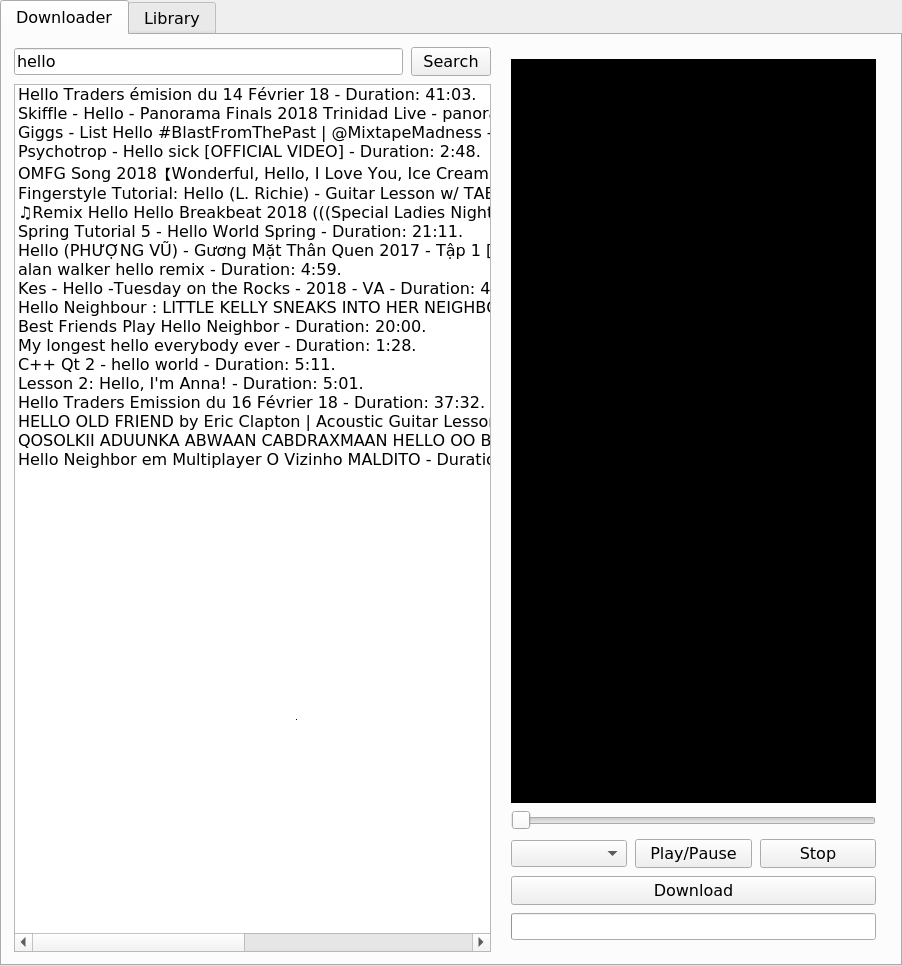
\includegraphics[width = 2in]{testPhotos/t1.png}} &
            \subfloat[Test id 3]{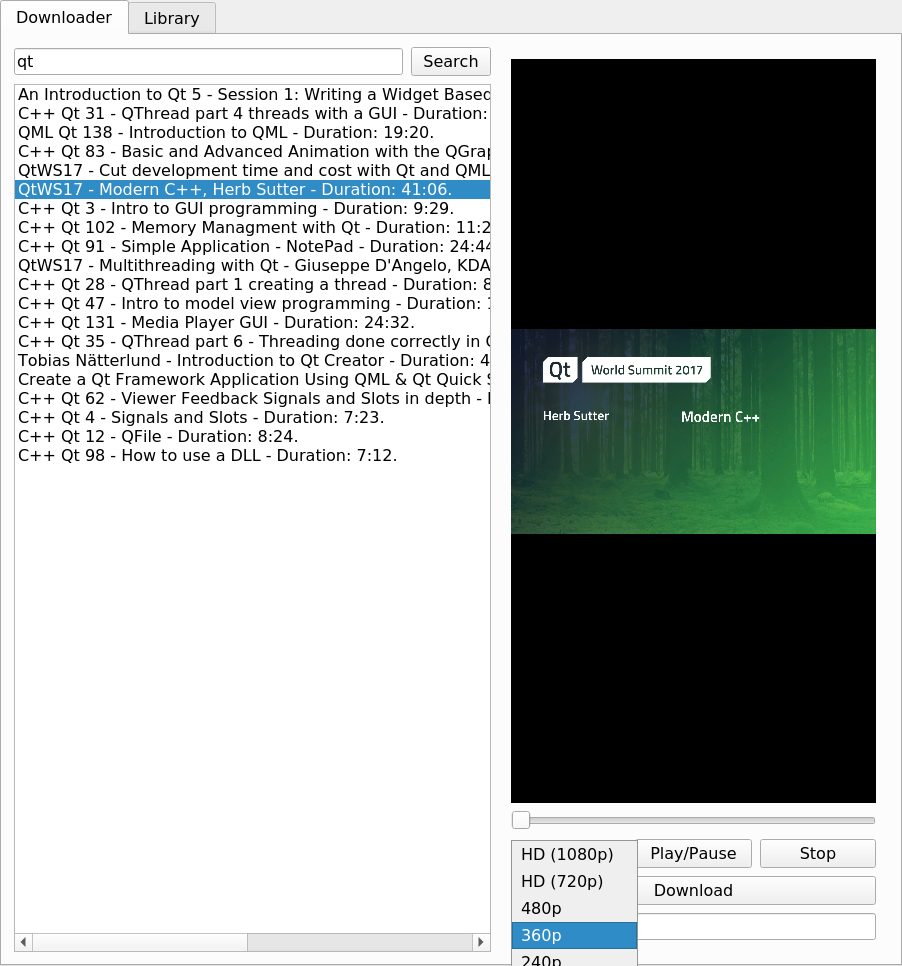
\includegraphics[width = 2in]{testPhotos/t3.png}} &
            \subfloat[Test id 4]{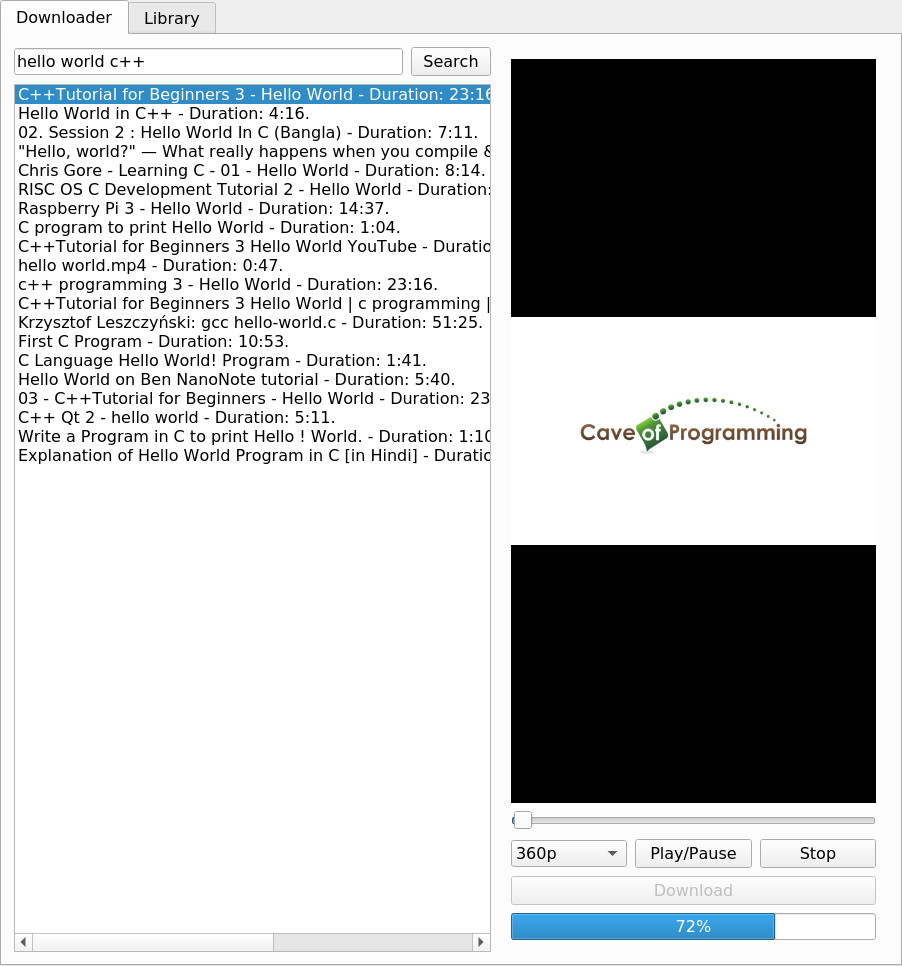
\includegraphics[width = 2in]{testPhotos/t4.png}} \\
            \subfloat[Test id 5]{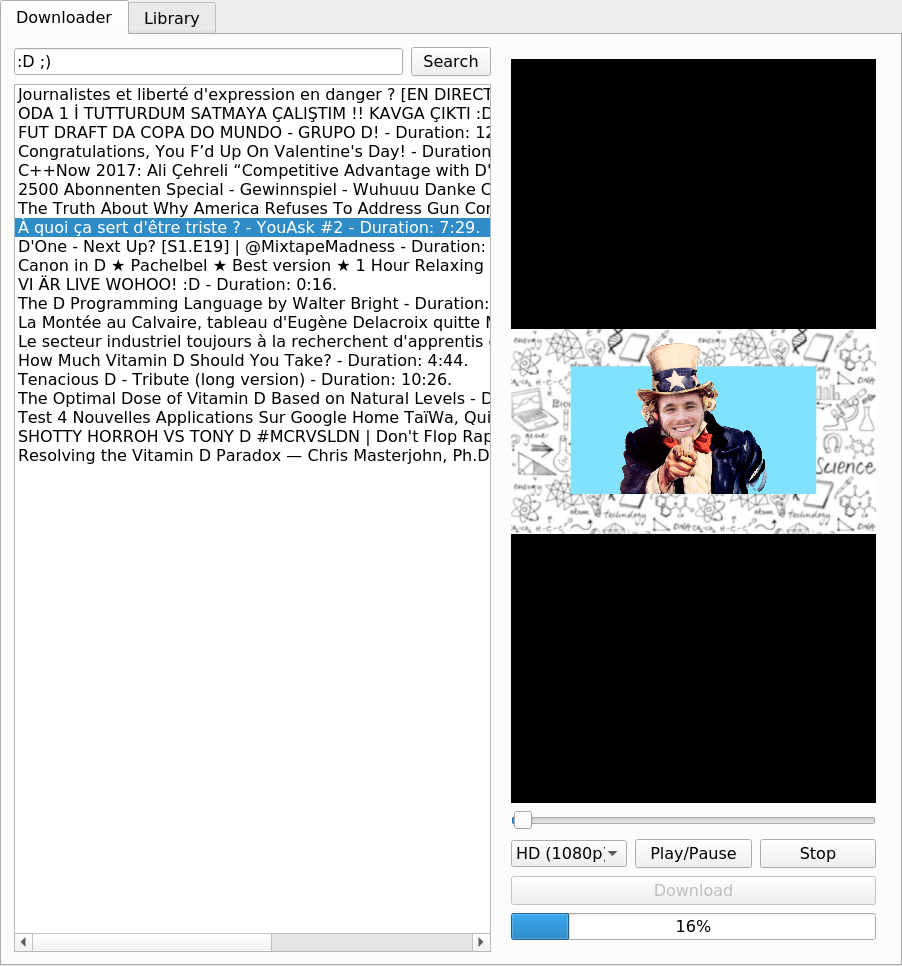
\includegraphics[width = 2in]{testPhotos/t5.png}} &
            \subfloat[Test id 6 and 7 before]{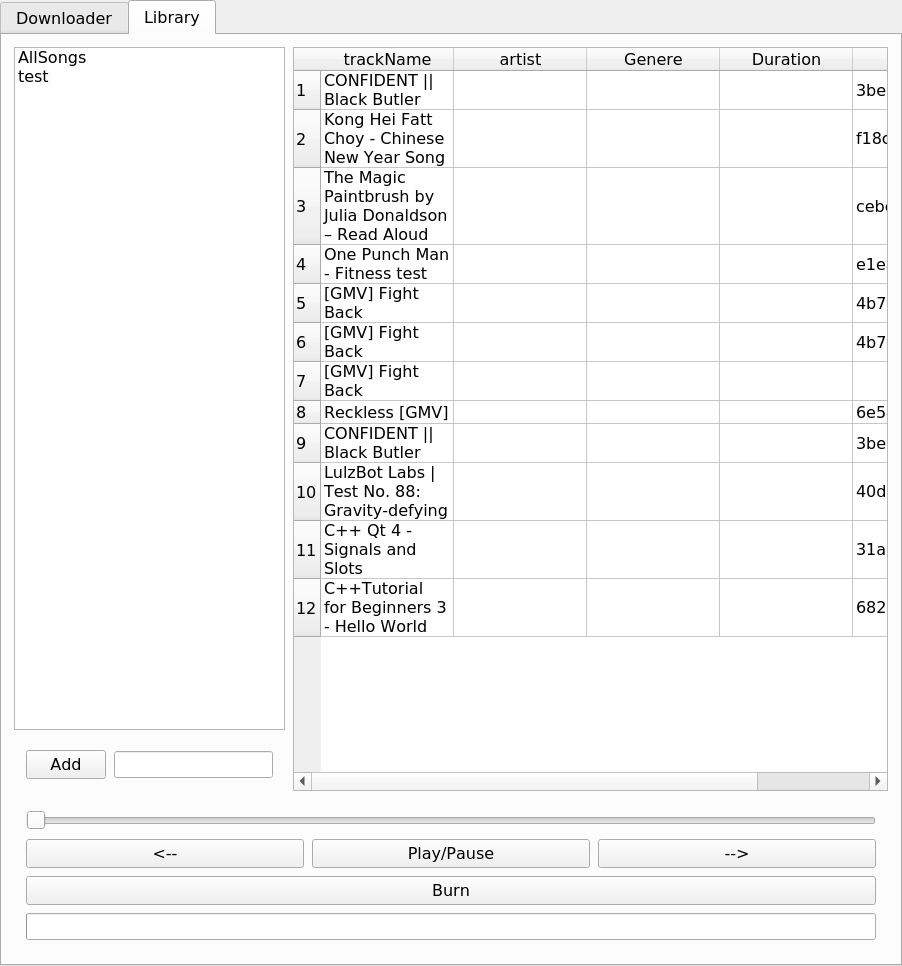
\includegraphics[width = 2in]{testPhotos/t6-1.png}} &
            \subfloat[Test id 6 after]{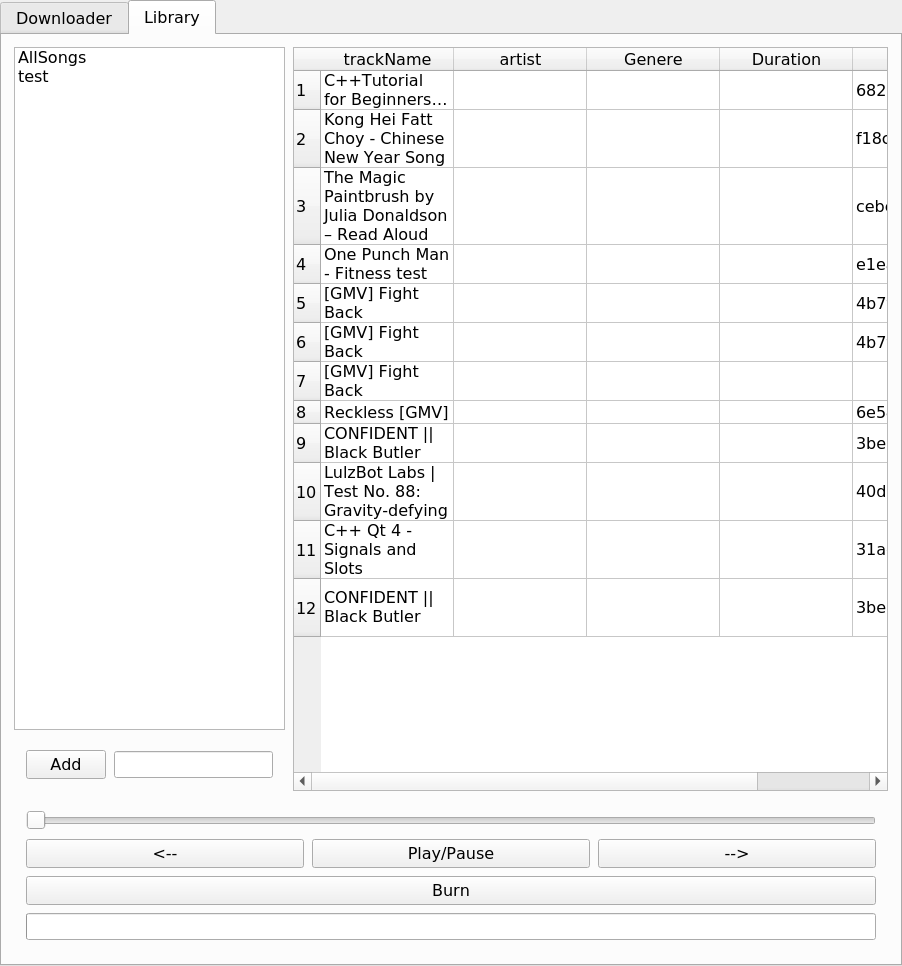
\includegraphics[width = 2in]{testPhotos/t6-2.png}} \\
            \subfloat[Test id 7 after]{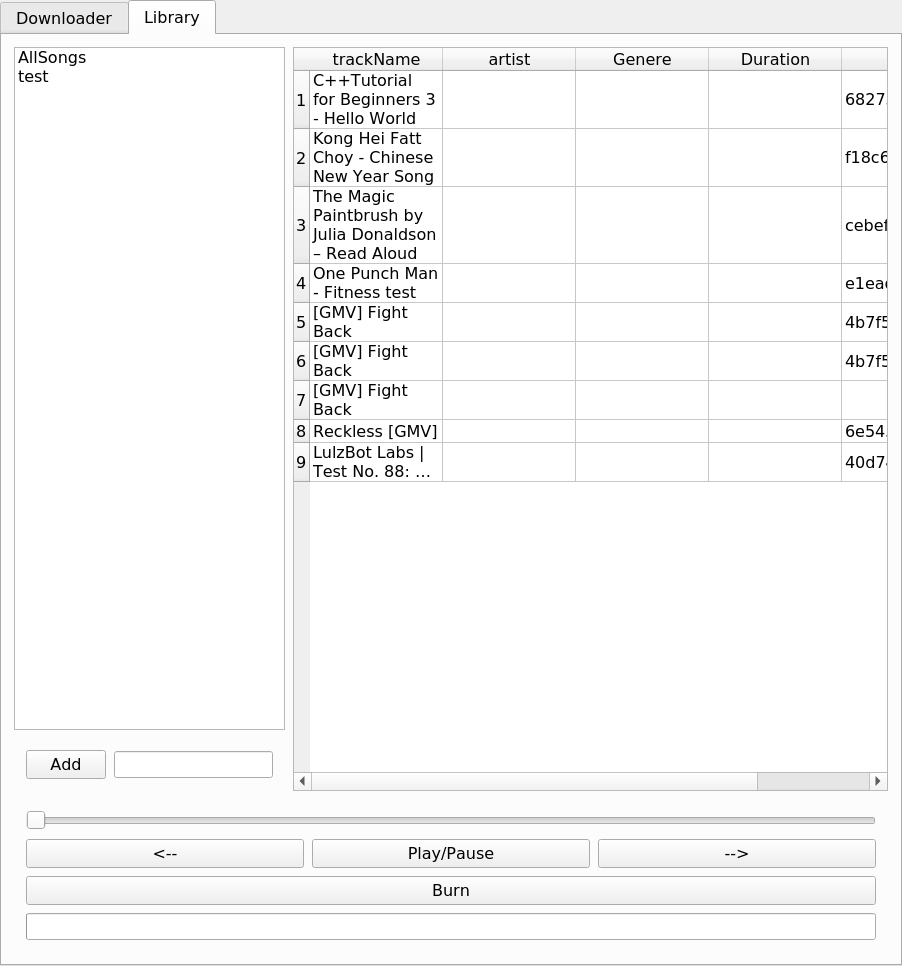
\includegraphics[width = 2in]{testPhotos/t7.png}} &
            \subfloat[Test id 8]{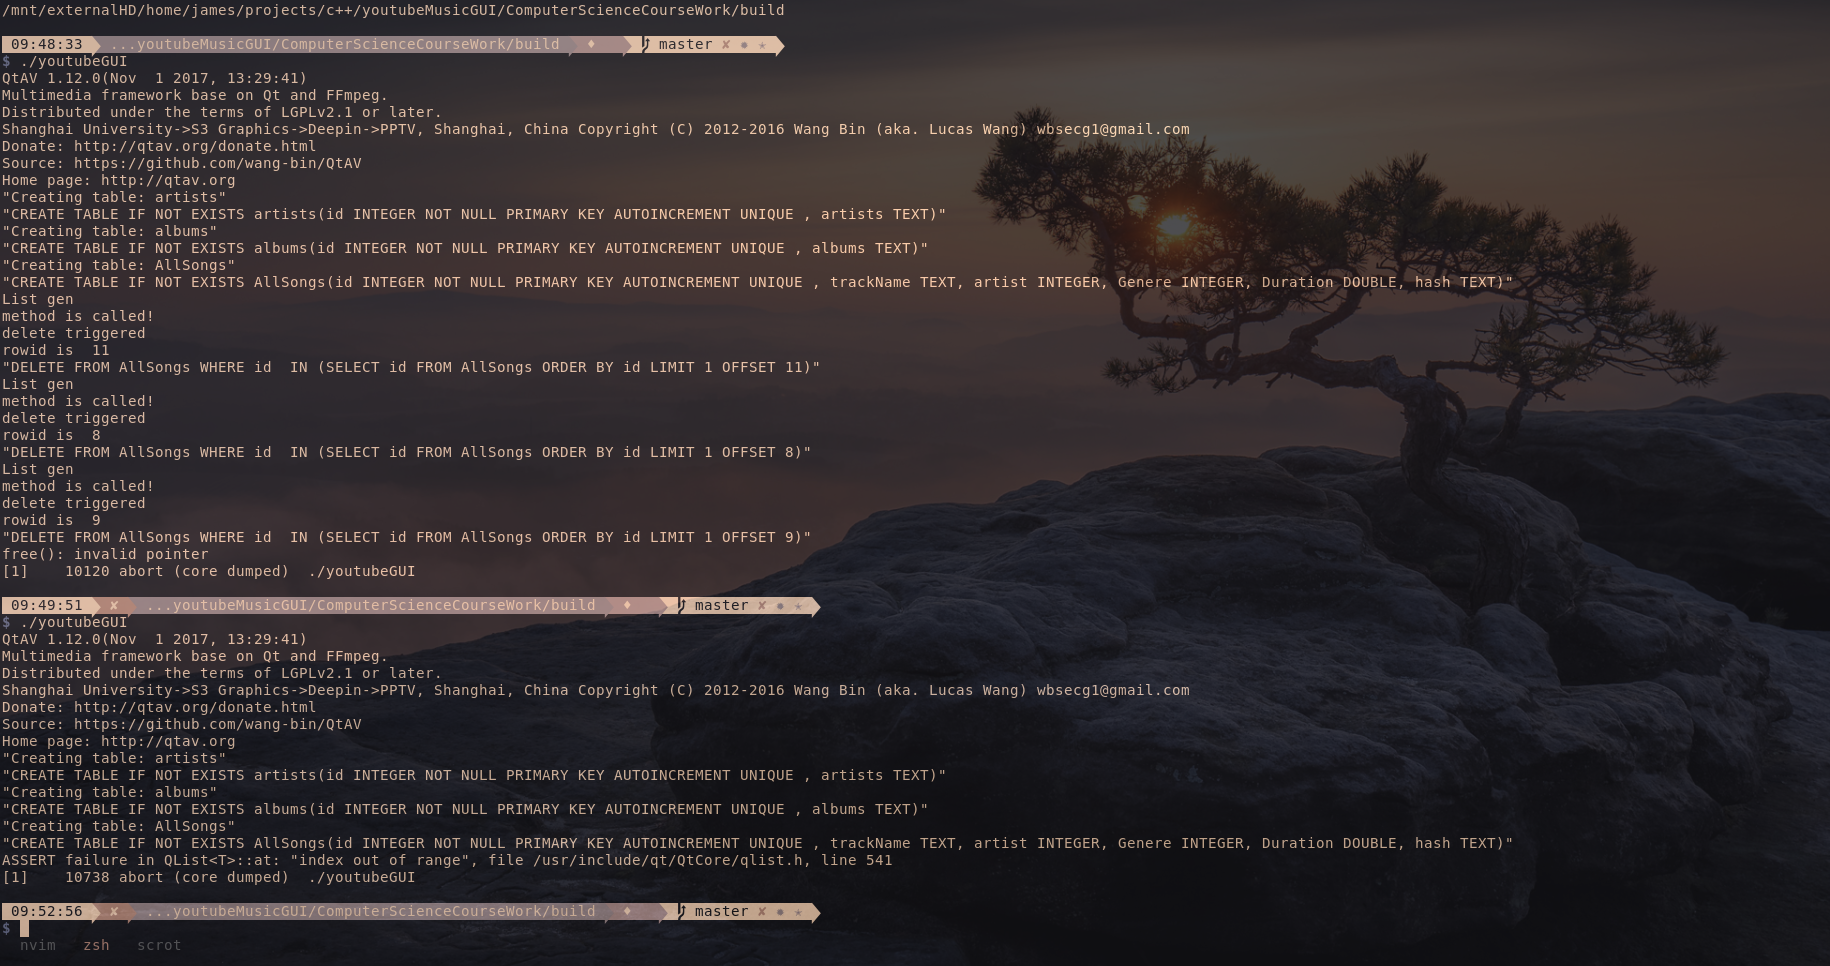
\includegraphics[width = 2in]{testPhotos/t8.png}} &
            \subfloat[Test id 9]{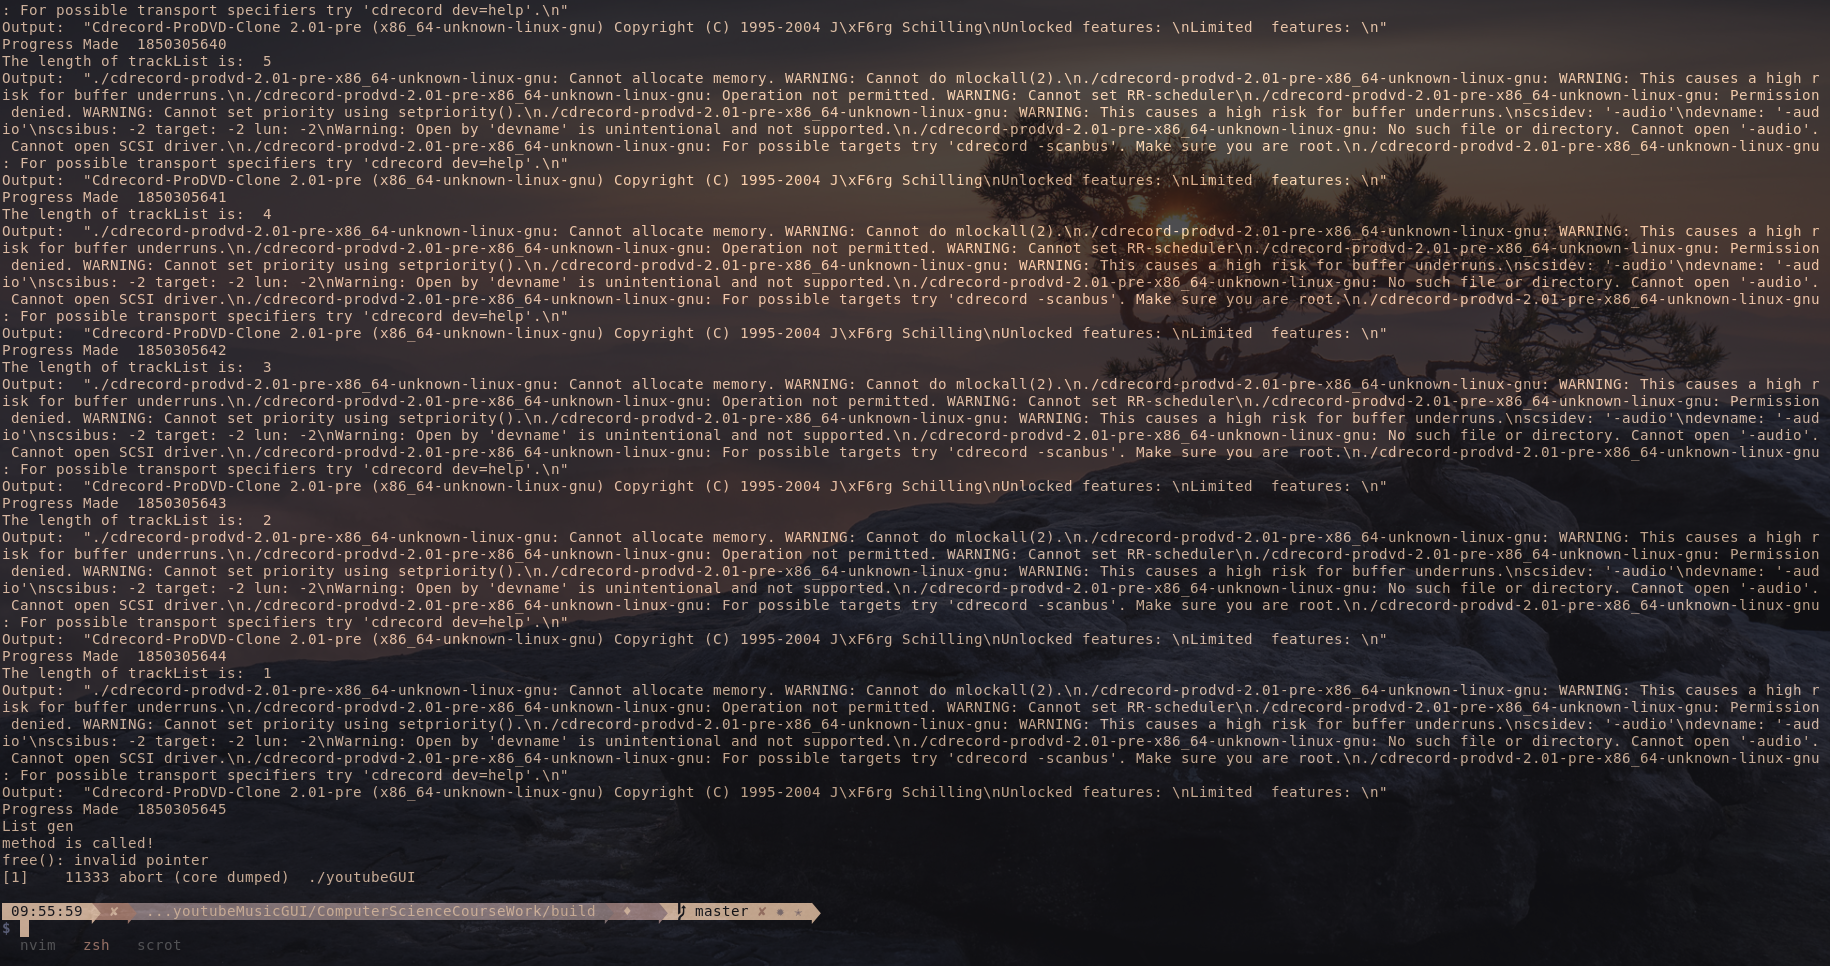
\includegraphics[width = 2in]{testPhotos/t9.png}} \\
        \end{tabular}
    \end{center}
    \caption{Testing Sample 1} \label{fig:tSample}
\end{figure}
\begin{figure}[H]
    \begin{center}
        \begin{tabular} {ccc}
            \hline
            \subfloat[Test id 10]{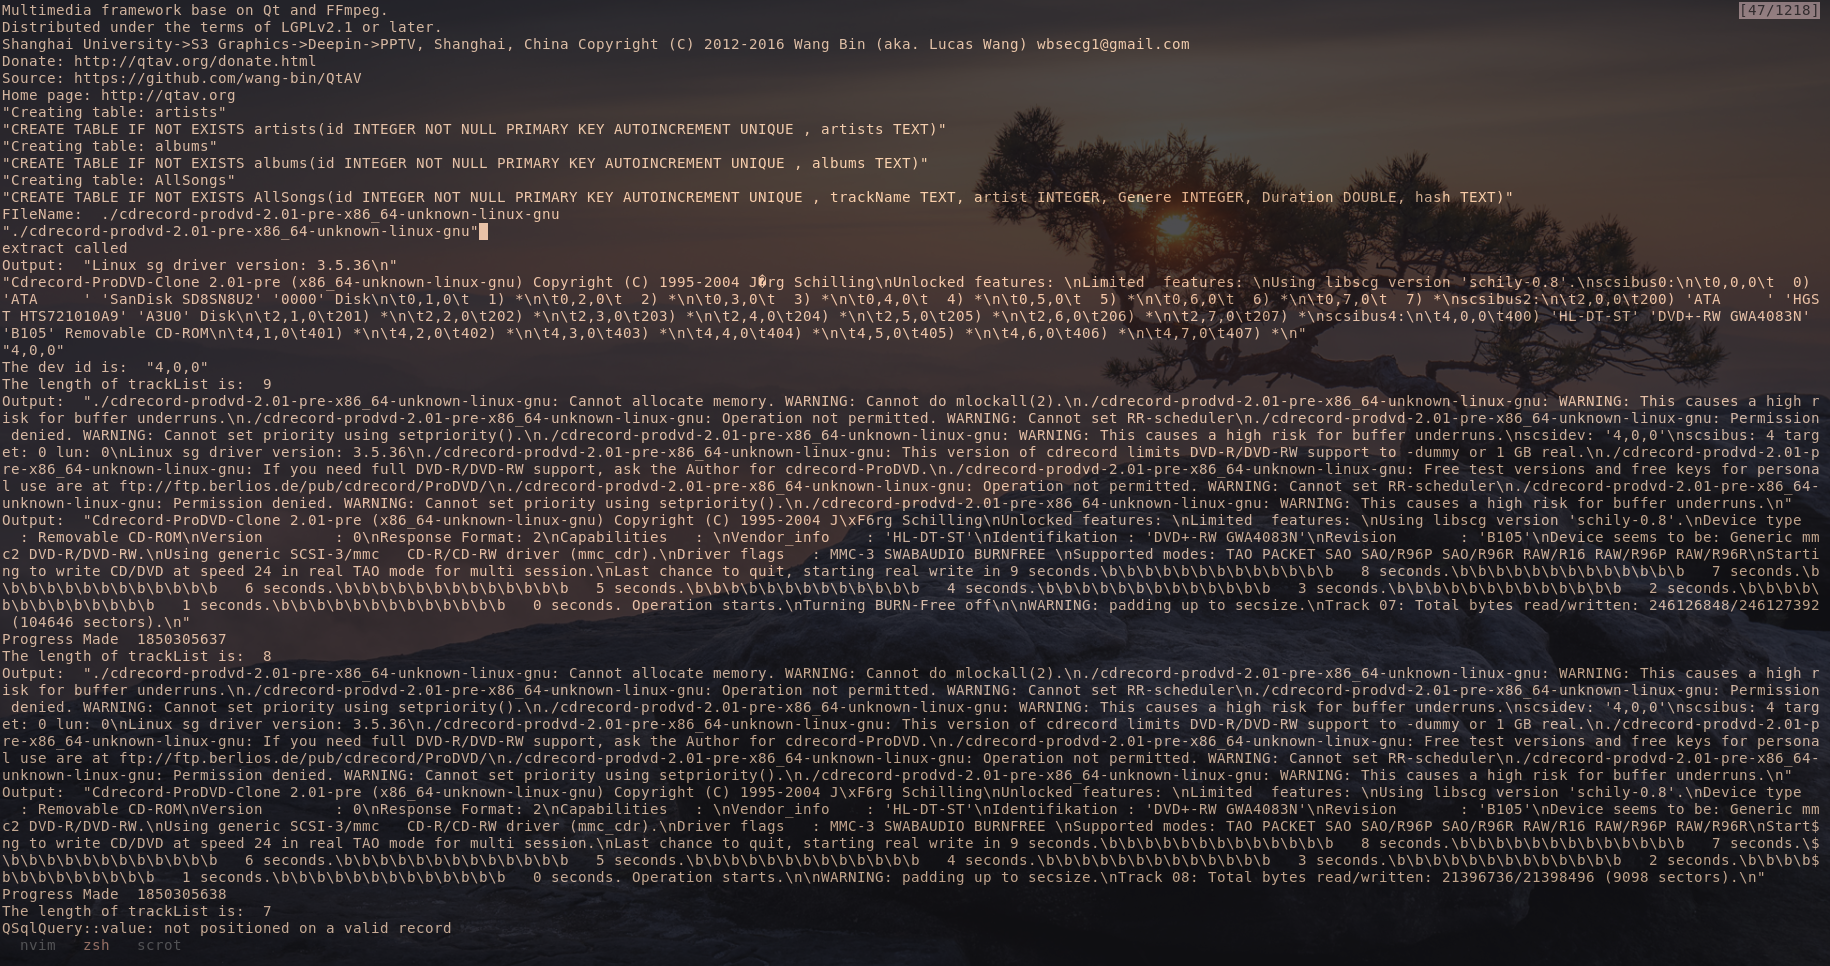
\includegraphics[width = 2in]{testPhotos/t10.png}} &
            \subfloat[Test id 11]{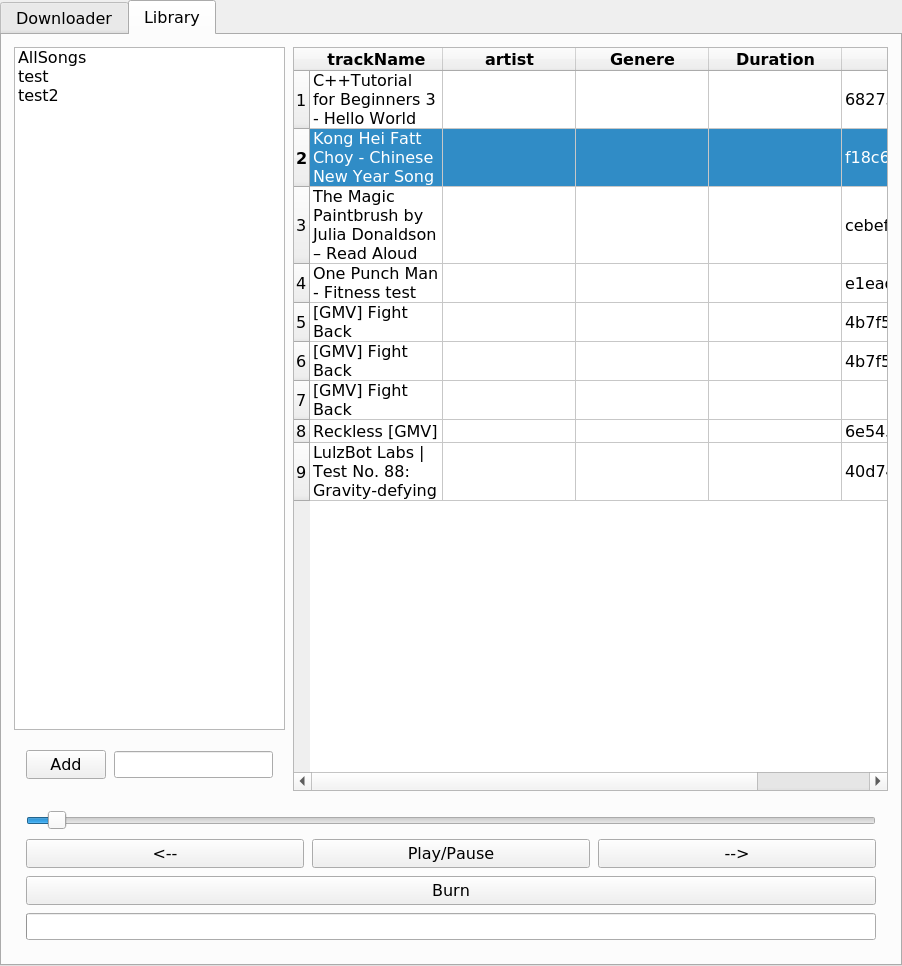
\includegraphics[width = 2in]{testPhotos/t11.png}}
        \end{tabular}
    \end{center}
    \caption{Testing Sample 1} \label{fig:tSample}
\end{figure}
\begin{thebibliography}{9}
\bibitem{e1}
    Test id 8,
    This test fails due to accessing an index in a list that was not available. This fail when trying to
    go to the next song when before selecting a playlist so it is likely caused by not having either index
    or tracklist properties set in PlayerWindow.cpp
\bibitem{e2}
    Test id 9,
    This test fails from not being able to access the CD drive on Linux due to insufficient permissions. Their
    is little I can do to resolve this issue apart from attempting to make an exception in the sudoers file for
    cdrecord.
\end{thebibliography}
\section{Evaluation}
I belive that the final program achieves the main objectives but work could be done to improve the stability
and reliability of the program. The final product also differs from my original design in many ways, particularly
with the burning process where I used a QProcess instead of a QThread. Another major change is the way that I
store the filename of the downloaded audio. I found that using the original file caused issues when I either
tried to convert it or burn it to a CD due to special characters acting in unpredictable ways. To get around this
issue I hashed the filename and store it in the database with the filename. This was so I could still present
a readable name to the user while still being able to find which hash belonged to which file.

I do belive that the system is effective as it can find copy right free content and download it at a decent
speed while avoiding things like ads and malware which the user would experience if she wanted to download
music off the web. Due to the drag and drop iteraction the system is easy to learn. How long this solution
will last for however might be a problem as youtube is likely to change and update in the future which
might make the current broken.

The ability to download music and store it was one of the original goals of this project and I think the
final solution performs well in this area. It is able to save the data in a temp file when downloading;
hash the name and save it in the folder and finally save it into a database for management purposes. Therefore
I think I have satisfied this objective. Another pre-planed goal was to be able to create playlists so that
the user can organise their. I think my project does this effectively by impleamenting tables as playlists
which gives the user full control over how they want the playlist to be. One of the more challanging
objectives that I think my application has had less success over is being able to burn the music
onto the disks through the application. Although it can perform this task it is quite slow at doing it
and on some systems like linux it requires additional permissions. Finally the last objective, it must
work on almost any enviroment without programs or libries being pre-installed. Due to the choice of programming
language and using the Qt library it completes this task excellently. The additional programs it uses, ffmpeg
and cdrecord, are well suited to this need by being completly cross-platform.


\subsection{User feedback}
\end{document}
